\documentclass[a4paper, 10 pt]{report}
\usepackage[T1]{fontenc}
\usepackage{comment}
\usepackage{booktabs}

\usepackage[english]{babel}
\usepackage{graphicx}
\usepackage{listings}
\usepackage{amsmath}
\usepackage[utf8]{inputenc}
\usepackage[tmargin=3cm,lmargin=3cm,rmargin=3cm,bmargin=3cm]{geometry}
\usepackage{fancyhdr}
\usepackage[yyyymmdd]{datetime}
\usepackage{array}
\usepackage{circuitikz}
\usepackage{siunitx}
\usepackage{longtable}
\usepackage{multirow}
\usepackage{capt-of}
\usepackage{float}
\usepackage{caption}
\usepackage{wrapfig}
\usepackage{subcaption}
\usepackage{verbatim}
\usepackage{epstopdf}
\usepackage{tikz-timing}
\usepackage{enumitem}
\usepackage{slashbox}
\usepackage{pgfplots}
\usepackage{adjustbox}
\usepackage{amssymb}
\usepackage{engtlc}
\usepackage{multicol}
\usepackage{import}
\usepackage{amsfonts}
%\usepackage{cite}
%\usepackage[numbered,autolinebreaks,framed]{mcode} %per mettere le impostazioni su come importare il codice Matlab
\usepackage{float} % per forzare la posizione delle immagini nel testo


\usepackage[numbered,autolinebreaks,framed]{mcode}	%framed for outlines
\lstset{breakatwhitespace=false}
\setlength{\columnseprule}{1pt}

\usetikztiminglibrary[rising arrows]{clockarrows}
\usepgfplotslibrary{external} 
\tikzexternalize
\newcommand{\datetime}{\today}
\newcolumntype{C}[1]{>{\centering\let\newline\\\arraybackslash\hspace{0pt}}m{#1}}
\newcommand\todo[1]{\textcolor{blue}{#1}}




\pagestyle{fancy}
\fancyhf{}
\renewcommand{\headrulewidth}{0.4pt} % optional
\renewcommand{\footrulewidth}{0.4pt} % optional
\fancyhead[C]{\nouppercase{\leftmark}}
\cfoot{\thepage}



\usepackage[hidelinks]{hyperref}




\begin{document}



%\begin{titlepage}
%	\vspace{2cm}
%	\centerline{
%		
\includegraphics[width=2cm]{./logopoli.jpg}}  
%	\vspace{0.5cm}
%	\centerline{\LARGE Politecnico di Torino}
%	\bigskip
%	
%	\vspace{4cm}
%	\centerline{\Huge\sf Pipelined Wallace Tree}
%	\bigskip
%	\centerline{\Huge\bfseries\sf Integrated system technology}
%	\vspace{2cm}
%	\centerline{\Large GROUP: 12}
%	\vspace{2cm}
%	\centerline{\Large Andrea Massa}
%	\vspace{0.2cm}
%	\centerline{\Large Giorgio Perrone}
%	\vspace{0.2cm}
%	\centerline{\Large Alberto Venzo}
%	\vspace{0.2cm}
%	\centerline{\Large Daniele Volpintesta}
%	\vspace{3cm}
%	
%\end{titlepage}
\begin{titlepage}
	
	\begin{figure}[h]
		\centering
		
\includegraphics[width = 5cm]{logopoli}
		\label{logo_polito}
	\end{figure}
	
	\begin{center}
		\textbf{{\LARGE POLITECNICO DI TORINO}}
	\end{center}
	
	\begin{center}
		\textbf{{\large Corso Di Laurea Magistrale in Ingegneria Elettronica}}
	\end{center}
	
	\begin{center}
		\rule{1\textwidth}{0.4pt}\\
	\end{center}
	
	\vspace{0 mm}
	
	\begin{center}
		\textbf{INTEGRATED SYSTEM TECHNOLOGY}
	\end{center}
	
	\vspace{5 mm}
	
	\begin{center}
		\textbf{\LARGE Project Report\\ Group 12} 
	\end{center}
	
	\vspace{20 mm}
	
	\begin{Large}
		\begin{center}
			\begin{tabular}{c c}
				\hline
				Students & Id. number \\ \hline
				Andrea Massa & 253271 \\ 
				Giorgio Perrone & 252969 \\ 
				Alberto Venzo & 249840 \\
				Daniele Volpintesta & 243764 \\ 
				\hline
			\end{tabular}
		\end{center}
	\end{Large}
	
	\vspace{40 mm}
	
	\begin{center}
		\rule{1\textwidth}{0.4pt}\\
	\end{center}
	
	\begin{center}
		\textbf{ACADEMIC YEAR 2018 - 2019}
	\end{center}
	
\end{titlepage}
\tableofcontents
\chapter{Pentium IV adder}


\section{Introduction}
The aim of this project is to create a model of Pentium IV adder in order to estimate its area, delay and power comsumption. For this purpose, a Matlab script has been implemented to derive and plot results. Simulations for 8, 12, 16, 20, 24, 28 and 32 bit cases are reported in this work.\\
In this project it has been supposed that any elementary logic gate necessary are available as external components. Each logic gate is assumed to be already characterized in terms of area, delay, input capacitances and leakage currents.\\
The approach for the design is structural: each block in the pentium IV is characterized like a black-box with its area, delay and power consumption. In this way the internal structure of any block can be changed without modifying anything else and then the Matlab script can be run with the previous settings. This could be very useful to make future improvements for more complex simulations and structural designs.\\



\section{Library logic gates}
The logic gates used in the Pentium IV adder are NAND2, NOR2, INV, XOR2 and the transmission gate (called for brevity "tgate"). In the table  \ref{library_logic_gates} are listed the gates with their parameters.

\begin{table}[H]
\begin{center}
\begin{tabular}{|c|c|c|c|c|}
\hline
GATE & AREA & INPUT & DELAY & AVERAGE LEAKAGE \\
TYPE &      & CAPACINTANCES &  & CURRENT \\ \hline
NAND2 & $A_{nand2}$ & $C_{in_{nand2}}$ & $\tau_{int_{nand2}}+\alpha_{nand2}\cdot C_L$ & $I_{leak_{nand2}}$ \\ \hline
NOR2 & $A_{nor2}$ & $C_{in_{nor2}}$ & $\tau_{int_{nor2}}+\alpha_{nor2}\cdot C_L$ & $I_{leak_{nor2}}$ \\ \hline
INV & $A_{inv}$ & $C_{in_{inv}}$ & $\tau_{int_{inv}}+\alpha_{inv}\cdot C_L$ & $I_{leak_{inv}}$ \\ \hline
XOR2 & $A_{xor2}$ & $C_{in_{xor2}}$ & $\tau_{int_{xor2}}+\alpha_{xor2}\cdot C_L$ & $I_{leak_{xor2}}$ \\ \hline
TGATE & $A_{tgate}$ & $C_{in1_{tgate}}, C_{in2_{tgate}}, C_{in3_{tgate}}$ & $\tau_{int_{tgate}}+\alpha_{tgate}\cdot C_L$ & $I_{leak_{tgate}}$ \\ \hline
\end{tabular}
\end{center}
\caption{library logic gates}
\label{library_logic_gates}
\end{table}

A brief explanation of the parameters is given before the adder analysis. For instance, the NAND2 gate can be considered. \\
$A_{nand2}$ is the area of the NAND2.\\
$I_{leak_{nand2}}$ is the average leakage current of the NAND2. The leakage current of a logic gate depends on the values of its inputs, therefore the average leakage current is a function of the input probabilities. For sake of semplicity, the average leakage current is computed by considering the probabilities of the inputs equal.\\
For the input capacitances and the delay of the NAND2 figure \ref{NAND2_gate} can be considered.

\begin{figure}[H]
\centering
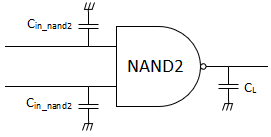
\includegraphics[width = 8cm]{pentium/nand2.png}
\caption{NAND2 gate}
\label{NAND2_gate}
\end{figure}

$C_{in_{nand2}}$ is the input capacitance in each input of the NAND2 gate.\\
The total delay of the NAND2 is 
$\tau_{int_{nand2}}+\alpha_{nand2}\cdot C_L$ where $\tau_{int_{nand2}}$ is the intrinsic delay of the NAND2 (the delay without load) while $\alpha_{nand2}\cdot C_L$ is the contribution that depends on the load $C_L$. The coefficient $\alpha_{nand2}$ depends on the sizes of the transistors inside the gate. The larger the transistors are, the smaller the delay is ($\alpha_{nand2}$ is smaller).\\
In the table, TGATE is the transmission gate. We will use the TGATE to make multiplexers. The TGATE is the only one in the table that has input capacitances depending on which input is considered (differently respect to a normal CMOS gate).\\
It is assumed that all the parameters in table  \ref{library_logic_gates} are given externally. In other words, the design is a function of the parameters reported in the table.\\
Also the supply voltage will be a input parameter because it depends on the technology adopted.\\





\section{Important assumptions in the design}\label{ciao}
To evaluate the dynamic power in the design the switching activity $E_{sw}$ for each node of the circuit has been assumed equal to one. This is a very pessimistic case that it will not happen in reality.\\
Evaluate the switching activity in each node is a very complex work. To do it the statistic of the inputs in our pentium IV should be known. Assuming $E_{sw}=1$ the dynamic power is therefore overestimated. For instance, the real value could be also one order of magnitude smaller. This means that the value of the dynamic power can be considered as an upper bound.\\
The working frequency that it has been used for the dynamic power is the inverse of the critical path of the Pentium IV adder (obviously the clock to output delay of a flip-flop, the setup time and the skew should be considered but this is also a simple estimation for power).\\
The leakage current in table \ref{library_logic_gates} is in the case that the input probabilities for each gate are the same as already said. Obviously this is not true in reality, therefore the value obtained for the static power will be not exactly. However the order of magnitude is expected reasonably correct. This simplification is done because it is too complex to obtain the real statistic of the inputs of each gate: several simulations should be performed in order to obtain the switching activity of each node.\\
To compute the delay of a path, all the delays of all gates in that particular path are summed. This means that, in table \ref{library_logic_gates}, the $50\%$ delay for each gate has been considered.





\section{Pentium IV adder design}
The 32-bit Pentium IV adder is constituted by two blocks as reported in figure \ref{pentiumIV}. The carry-merge sparse tree computes the carry bit in position 4, 8, 12, 16, 20, 24, 28 and 32. The carry-select sum generator computes the sum bit.\\
\begin{figure}[H]
\centering
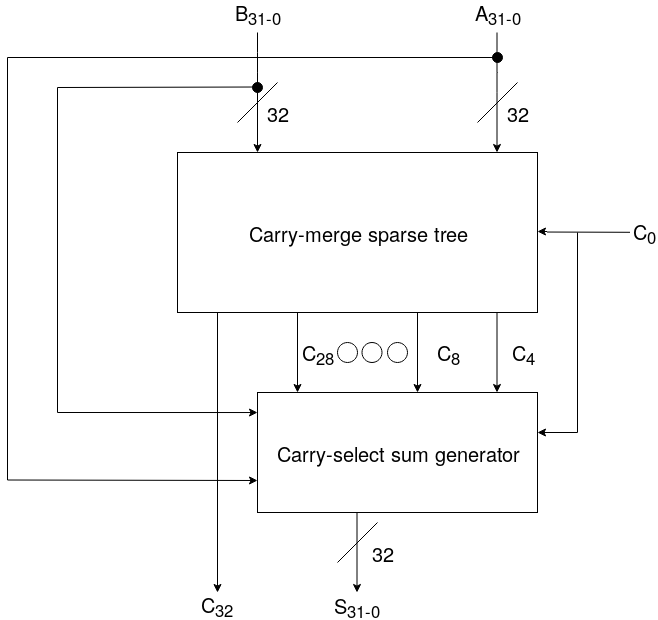
\includegraphics[width = 10 cm]{pentium/pentiumIV.png}
\caption{Pentium IV adder}
\label{pentiumIV}
\end{figure}
In the following sections these two blocks will be detailed. A bottom-up approach has been used to complete this design.





\subsection{Carry-select sum generator design}
In this subsection the carry-select sum generator is designed. 


\subsubsection{Full adder}
In Figure \ref{fa_black_box} it is shown the symbol of the full adder while in Figure \ref{fa_interno} its internal circuit is shown.


\begin{figure}[H]
\centering
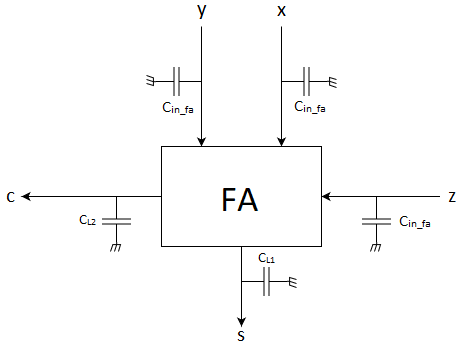
\includegraphics[width = 8cm]{pentium/fa_black_box.png}
\caption{Symbol of full adder}
\label{fa_black_box}
\end{figure}

\begin{figure}[H]
\centering
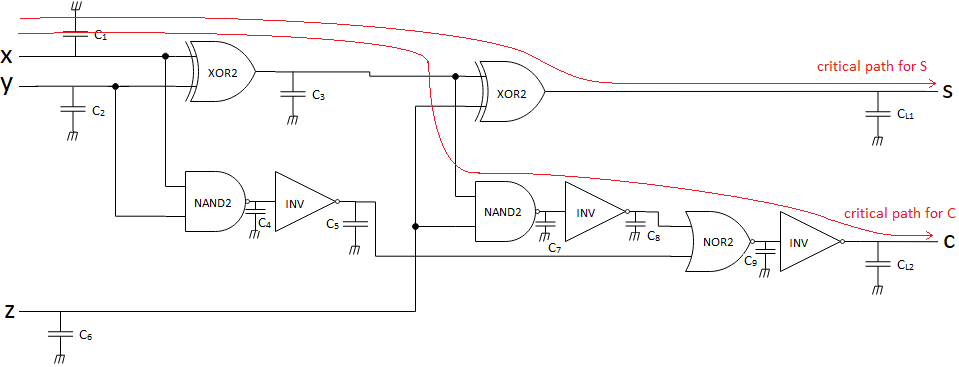
\includegraphics[width = 14cm]{pentium/fa_interno.png}
\caption{Internal full adder circuit}
\label{fa_interno}
\end{figure}

The full adder area is given by:
\begin{equation}
A_{FA}=2A_{xor2}+2A_{nand2}+A_{nor2}+3A_{inv}
\end{equation}
The leakage current is:
\begin{equation}
I_{leak_{FA}}=2I_{leak_{xor2}}+2I_{leak_{nand2}}+I_{leak_{nor2}}+3I_{leak_{inv}}
\end{equation}
The static power is:
\begin{equation}
P_{stat_{FA}}=V_{DD}\cdot I_{leak_{FA}}
\end{equation}
For the dynamic power, as said, it has been assumed that the switching activity $E_{sw}$ of all the nodes in the circuit is equal to one. Therefore it is possible to write:
\begin{equation}
P_{dyn_{FA}}=V_{DD}^2f_{CLK}E_{sw}(C_3+C_4+C_5+C_7+C_8+C_9)
\end{equation}
NOTE: for the dynamic power only the internal nodes are considered, which is that the input and output ones are not taken into account. The contribution of the input and output nodes will be considered when the FA-block will be used to create others blocks.\\
Looking at figure \ref{fa_interno} it is possible to see that:
\begin{equation}
C_1=C_2=C_3=C_6=C_{in_{xor2}}+C_{in_{nand2}}
\end{equation}
\begin{equation}
C_4=C_7=C_9=C_{in_{inv}}
\end{equation}
\begin{equation}
C_5=C_8=C_{in_{nor2}}
\end{equation}

Thus:
\begin{equation}
P_{dyn_{FA}}=V_{DD}^2f_{CLK}E_{sw}(C_{in_{xor2}}+C_{in_{nand2}}+3C_{in_{inv}}+2C_{in_{nor2}})
\end{equation}

The intrinsic delay (the delay without load) of the output $S$ is:
\begin{equation}
\tau_{int_{FA_{S}}} = \tau_{int_{xor2}}+\alpha_{xor2}C_3+\tau_{int_{xor2}} = 2\tau_{int_{xor2}}+\alpha_{xor2}(C_{in_{xor2}}+C_{in_{nand2}})
\end{equation}

The $\alpha$ parameter is:
\begin{equation}
\alpha_{FA_{S}}=\alpha_{xor2}
\end{equation}

Thus the total delay of $S$ (considering the load) is $\tau_{int_{FA_{S}}}+\alpha_{FA_{S}}C_{L1}$.\\\\
Analogously for the output $C$ it is obtained:
\begin{equation}
\tau_{int_{FA_{C}}} = \tau_{int_{xor2}}+\alpha_{xor2}C_3+\tau_{int_{nand2}}+\alpha_{nand2}C_7+\tau_{int_{inv}}+\alpha_{inv}C_8+\tau_{int_{nor2}}+\alpha_{nor2}C_9+\tau_{int_{inv}}
\end{equation}

\begin{equation}
\alpha_{FA_{C}}=\alpha_{inv}
\end{equation}

The delay of $C$ considering the load will be $\tau_{int_{FA_{C}}}+\alpha_{FA_{C}}C_{L2}$.\\\\

The input capacitances of the full adder are:
\begin{equation}
C_{in_{x}}=C_{in_{y}}=C_{in_{z}}=C_{in_{FA}}=C_{in_{xor2}}+C_{in_{nand2}}
\end{equation}





\subsubsection{4-bit ripple carry adder}
In Figure \ref{rca4_black_box} it is shown the symbol of the 4-bit ripple carry adder while in Figure \ref{rca4_interno} its internal circuit is shown.


\begin{figure}[H]
\centering
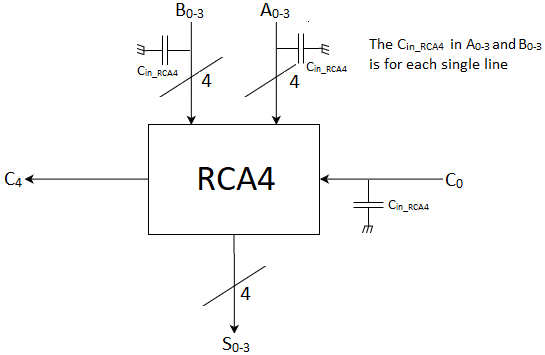
\includegraphics[width = 10cm]{pentium/rca4_black_box.png}
\caption{symbol of 4-bit ripple carry adder}
\label{rca4_black_box}
\end{figure}

\begin{figure}[H]
\centering
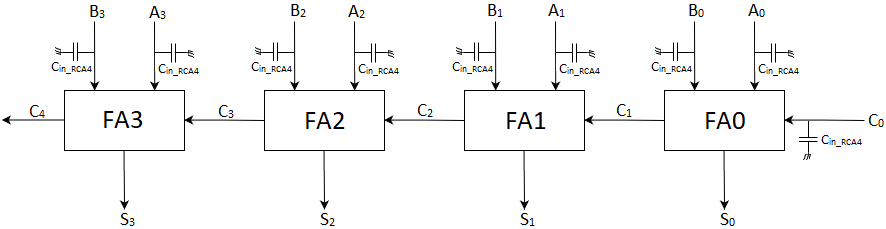
\includegraphics[width = 14cm]{pentium/rca4_interno_copia.png}
\caption{internal circuit of 4-bit ripple carry adder}
\label{rca4_interno}
\end{figure}

The  area of 4-bit ripple carry adder is given by:
\begin{equation}
A_{RCA4}=4A_{FA}
\end{equation}
The leakage current is:
\begin{equation}
I_{leak_{RCA4}}=4I_{leak_{FA}}
\end{equation}
The static power is:
\begin{equation}
P_{stat_{RCA4}}=V_{DD}\cdot I_{leak_{RCA4}}
\end{equation}

Just as in the case of the full adder, in order to compute the dynamic power only the internal nodes have been considered:
\begin{equation}
P_{dyn_{RCA4}}=V_{DD}^2f_{CLK}E_{sw}(3C_{in_{FA}})+4P_{dyn_{FA}}
\end{equation}
NOTE: the term $4P_{dyn_{FA}}$ is for the internal nodes of the FAs.\\\\
To compute the delay, it can be observed that the delay to generate the 4 sum bits ($S_0, S_1, S_2$ and $S_3$) is the main concern. This is why the output carry ($C_4$) will be generated by the tree. Thus the delay of RCA4 to be considered is the delay to generate $S_3$. The intrinsic delay (that without load) can be written as:

\begin{equation}
\tau_{int_{RCA4}} = 3\tau_{int_{FA_{C}}}+\alpha_{FA_{C}}(3C_{in_{FA}})+\tau_{int_{FA_{S}}}
\end{equation}

For the alpha coefficient it is derived that:
\begin{equation}
\alpha_{RCA4}=\alpha_{FA_{S}}
\end{equation}

The input capacitances for the carry input ($C_0$) and for each line of $A_{0-3}$ and $B_{0-3}$ is the same and equal to:
\begin{equation}
C_{in_{RCA4}}=C_{in_{FA}}
\end{equation}





\subsubsection{Transmission gate}
The transmission gate has been used to make multiplexers. Using transmission gates to implement MUXs, instead of normal CMOS gates, is in fact a good solution in terms of area, delay and power consuption.\\
In Figure \ref{tgate_black_box} it is shown the symbol of the transmission gate while in figure \ref{tgate_interno} its internal circuit.

\begin{figure}[H]
\centering
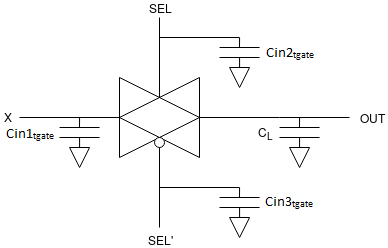
\includegraphics[width = 8 cm, height = 5 cm]{pentium/transmission_gate_black_box.png}
\caption{Symbol of the transmission gate}
\label{tgate_black_box}
\end{figure}

\begin{figure}[H]
\centering
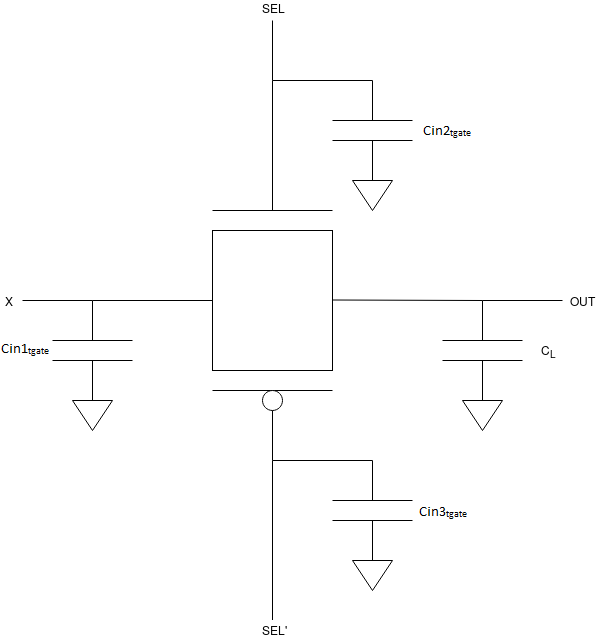
\includegraphics[width = 9 cm, height = 8 cm]{pentium/transmission_gate_interno.png}
\caption{Internal circuit of the transmission gate}
\label{tgate_interno}
\end{figure}

From Figure \ref{tgate_interno} it can be seen that the input capacitances of the transmission gate $C_{in1_{tgate}}$, $C_{in2_{tgate}}$ and $C_{in3_{tgate}}$ can be different. As said previously their values are given externally.\\
Also the area $A_{tgate}$ and the leakage current $I_{leak_{tgate}}$ are given.\\
The delay of the transmission gate is the time required for the signal at the input $X$ to reach the output node ($OUT$) when the two transistors become ON. This delay is equal to $\tau_{int_{tgate}}+\alpha_{tgate}\cdot C_L$ where $\tau_{int_{tgate}}$ and $\alpha_{tgate}$ are both given.





\subsubsection{Multiplexer 2:1}
From the transmission gate described before, a 2:1 way multiplexer (mux) can be designed and characterized. Figure \ref{fig:2to1mux} reports the designed mux.

\begin{figure}[H]
\centering
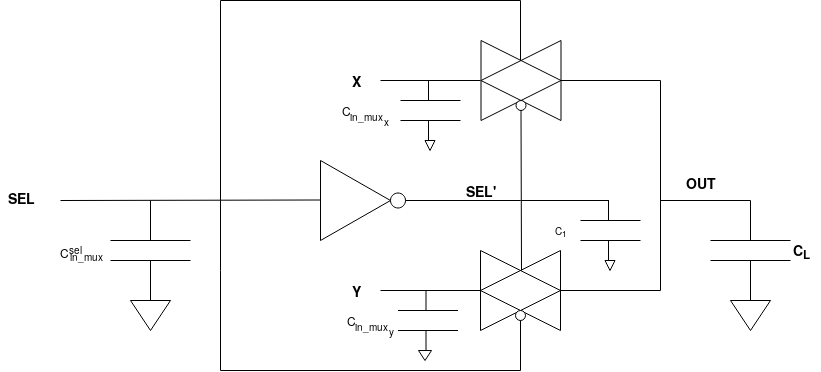
\includegraphics[width = 11.5 cm, height = 6 cm]{pentium/mux2.png}
\caption{2:1 way multiplexer implementation with transmission gates}
\label{fig:2to1mux}
\end{figure}

The black-box model used for the multiplexer is the one in figure \ref{fig:mux_black_box}.

\begin{figure}[H]
\centering
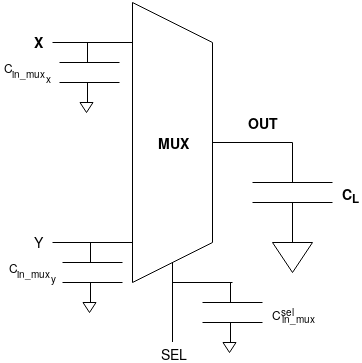
\includegraphics[width = 8 cm, height = 7 cm]{pentium/mux_schematic.png}
\caption{Multiplexer 2:1 symbol}
\label{fig:mux_black_box}
\end{figure}

%%%%%%%%%%%%%%%%%% Mux Formulas %%%%%%%%%%%%%%%%%%%%

 The multiplexer area is given by:
\begin{equation}
A_{mux} = A_{inv} + 2 A_{tgate}
\end{equation}
The leakage current is given by:
\begin{equation}
I_{leak_{mux}} = I_{leak_{inv}} + 2 I_{leak_{tgate}}
\label{eq:leak_cur_mux}
\end{equation}
The static power is
\begin{equation}
P_{stat_{mux}} = V_{DD} I_{leak_{mux}}
\end{equation}
Looking at the figure \ref{fig:2to1mux}, the dynamic power can be derived:
\begin{equation}
P_{dyn_{mux}} = V_{DD}^2 f_{CLK} E_{sw} C_1 
\end{equation}
Since $C_1 = C_{in2_{tgate}} + C_{in3_{tgate}}$ it is possible to obtain:
\begin{equation}
P_{dyn_{mux}} =  V_{DD}^2 f_{CLK} E_{sw}  (C_{in2_{tgate}} + C_{in3_{tgate}})
\end{equation}
The intrinsic delay (the delay without load) for the mux is:
\begin{equation}
\tau_{int_{mux}} = \tau_{int_{inv}} + \alpha_{inv} C_1 +\tau_{int_{tgate}}
\end{equation}
Replacing $C_1$
\begin{equation}
\tau_{int_{mux}} = \tau_{int_{inv}} + \alpha_{inv} (C_{in2_{tgate}} + C_{in3_{tgate}}) + \tau_{int_{tgate}}
\end{equation}

The $\alpha$ coefficient is:
\begin{equation}
\alpha_{mux} = \alpha_{tgate}
\end{equation}
Thus the overall delay is $\tau_{int_{mux}} + \alpha_{mux} C_L$. The input capacitance seen from the inputs X or Y is given by:
\begin{equation}
C_{in_{mux}}^{input} = C_{in_{mux_x}} = C_{in_{mux_y}} = C_{in1_{tgate}} 
\end{equation}
while the input capacitance seen from the select input is:
\begin{equation}
C_{in_{mux}}^{sel} = C_{in_{inv}} + C_{in2_{tgate}} + C_{in3_{tgate}}
\end{equation}





\subsubsection{Multiplexer 2:1 for M-length signal vectors}
In the Pentium IV adder design is useful a compact rappresentation of a selector which takes two vectors with a length equal to M and takes one of them to the output. Figure \ref{fig:M_sig_length_2to1mux} shows the implementation of such mux (called for brevity M-mux), while figure \ref{fig:mux_black_box_m} reports the black-box symbol.

\begin{figure}[H]
\centering
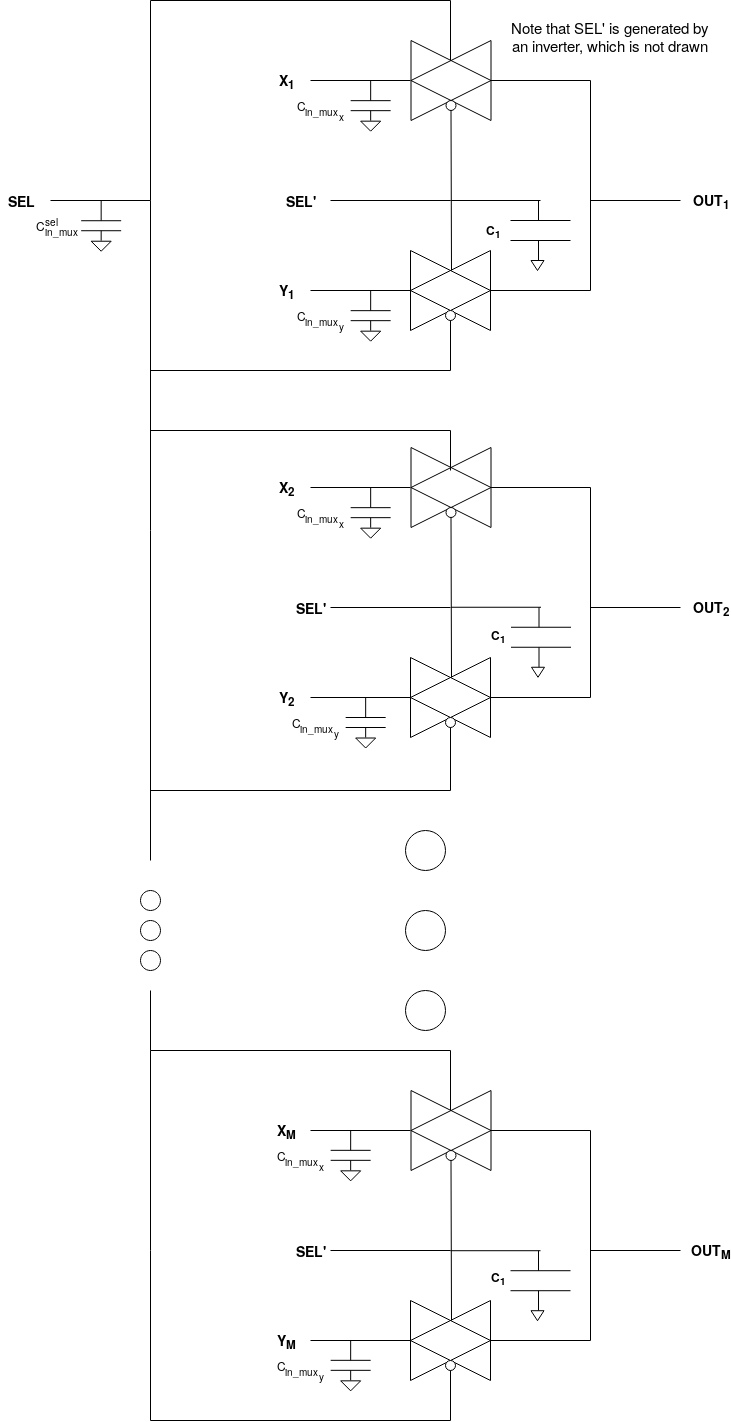
\includegraphics[width = 8 cm, height = 14 cm]{pentium/four_2to1_mux.png}
\caption{Mux 2:1 with M-bit inputs}
%\caption{implementation of a M-signal-length 2 to 1 mux}
\label{fig:M_sig_length_2to1mux}
\end{figure}

\begin{figure}[H]
\centering
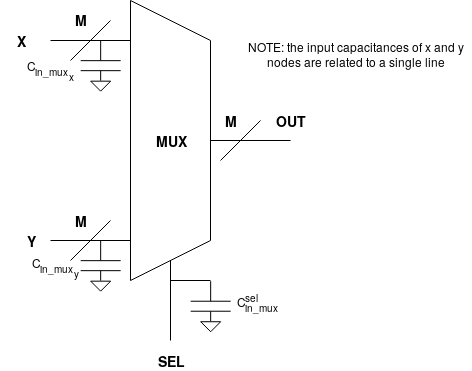
\includegraphics[width = 8 cm, height = 6 cm]{pentium/mux_schematic_m.png}
%\caption{mux for m-length signal block symbol}
\caption{Symbol of mux 2:1 with M-bit inputs}
\label{fig:mux_black_box_m} 
\end{figure}

%%%%%%%%%%%%%%%%%%%%%%%%%%%%%%%%%%%%%%%%%%%%%%%%%%%
%% Generalized mux formulas
%%%%%%%%%%%%%%%%%%%%%%%%%%%%%%%%%%%%%%%%%%%%%%%%%%%
Since in figure \ref{fig:M_sig_length_2to1mux} the SEL' signal is generated by an inverter which is not drawn, the area of the M-mux is:
\begin{equation}
A_{M-mux} = A_{inv} + 2M A_{tgate}
\end{equation}

The leakage current is given by:
\begin{equation}
I_{leak_{M-mux}} = I_{leak_{inv}} + 2M I_{leak_{tgate}}
\end{equation}

The static power is given by:
\begin{equation}
P_{stat_{M-mux}} = V_{DD} I_{leak_{M-mux}}
\end{equation}

The dynamic power is given by:
\begin{equation}
P_{dyn_{M-mux}} = V_{DD}^2 f_{CLK} E_{sw} \cdot M (C_{in2_{tgate}} + C_{in3_{tgate}})
\end{equation}

The intrinsic delay is:
\begin{equation}
\tau_{int_{M-mux}} = \tau_{int_{inv}} + \alpha_{inv} M (C_{in2_{tgate}} + C_{in3_{tgate}}) + \tau_{int_{tgate}}
\end{equation}

The $\alpha$ coefficient for the M-mux is: 
\begin{equation}
\alpha_{M-mux} = \alpha_{tgate}
\end{equation}

%Figure \ref{fig:m_2to1_mux_capacitance_schematic} shows the equivalent capacitances which has to be taken into account when the m-mux is used with reference to the 2 to 1 mux.

%\begin{figure}[H]
%\centering
%\includegraphics[width = 9 cm, height = 3 cm]{m_2to1_mux_capacitance_schematics.png}
%\caption{m-mux equivalent circuit for capacitance calculation.}
%\label{fig:m_2to1_mux_capacitance_schematic}
%\end{figure}

The input capacitances for each line of the x and y inputs are:
\begin{equation}
C_{in_{M-mux}}^{input} = C_{in_{mux_x}} = C_{in_{mux_y}} = C_{in1_{tgate}} 
\end{equation}
while the input capacitance seen from the select input is:
\begin{equation}
C_{in_{M-mux}}^{sel} = C_{in_{inv}} + M( C_{in2_{tgate}} + C_{in3_{tgate}})
\end{equation}





\subsubsection{Carry-select block}
The schematic of the carry-select block and its corresponding black box are reported in Figure \ref{fig:carry_select_schematic_bb}.

\begin{figure}[H]
\centering
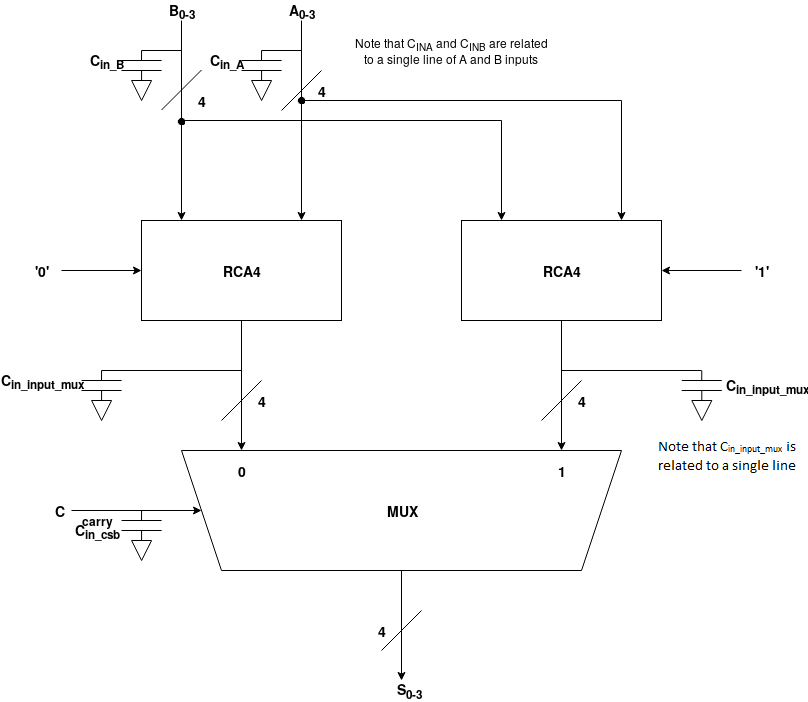
\includegraphics[width = 6 cm, height = 7 cm]{pentium/carry_select_adder_schematic.png}
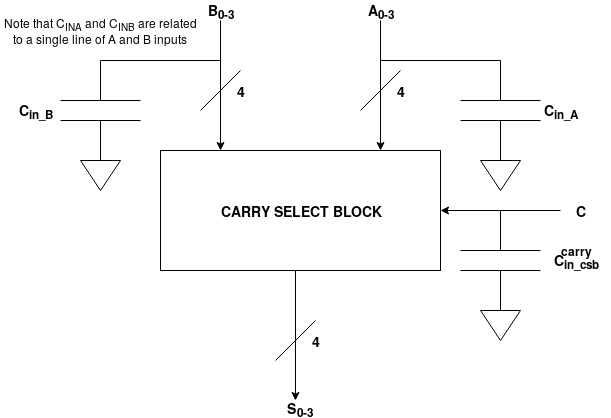
\includegraphics[width = 6 cm, height = 7 cm]{pentium/carry_select_adder_black_box.png} 
\caption{Carry-select block schematic view and block symbol}
\label{fig:carry_select_schematic_bb}
\end{figure}

The area of the carry-select block is given by:
\begin{equation}
A_{csb} = 2A_{RCA4} + A_{4-mux} 
\end{equation}

The leakage current is:
\begin{equation}
I_{leak_{csb}} = 2I_{leak_{RCA4}} + I_{leak_{4-mux}}
\end{equation}

The static power is given by:
\begin{equation}
P_{stat_{csb}} = V_{DD} I_{leak_{csb}} 
\end{equation}

The dynamic power is given by:
\begin{equation}
P_{dyn_{csb}} = V_{DD}^2 f_{CLK} E_{sw} (8 C_{in_{4-mux}}^{input}) + 2P_{dyn_{RCA4}} + P_{dyn_{4-mux}}
\end{equation}

Assuming that all the inputs $A_{0-3}$, $B_{0-3}$ and $C$ are stable, the delay is that of the path from $A_{0-3}$ and $B_{0-3}$ to $S_{0-3}$. Therefore the intrinsic delay (the delay without load) is:
\begin{equation}
\tau_{int_{csb}} = \tau_{int_{RCA4}} + \alpha_{RCA4} C_{in_{4-mux}}^{input} + \tau_{int_{4-mux}}
\end{equation}
The $\alpha$ coefficient of the carry-select block is:
\begin{equation}
\alpha_{csb} = \alpha_{4-mux}
\end{equation}

The input capacitance of a single input line ($A_{0-3}$ or $B_{0-3}$) is:
\begin{equation}
C_{in_{csb}}^{input} = C_{in_B} = C_{in_A} = 2 C_{in_{RCA4}}
\end{equation}
The carry input capacitance of the carry-select block is
\begin{equation}
C_{in_{csb}}^{carry} = C_{in_{4-mux}}^{sel}
\end{equation}





\subsubsection{Carry-select sum generator}
Carry-select sum generator (cssg) schematic is reported in figure \ref{fig:cssg_schematic} and its black box symbol in figure \ref{fig:cssg_bb}. In these figures the number of bits is set to 32.

\begin{figure}[H]
\centering
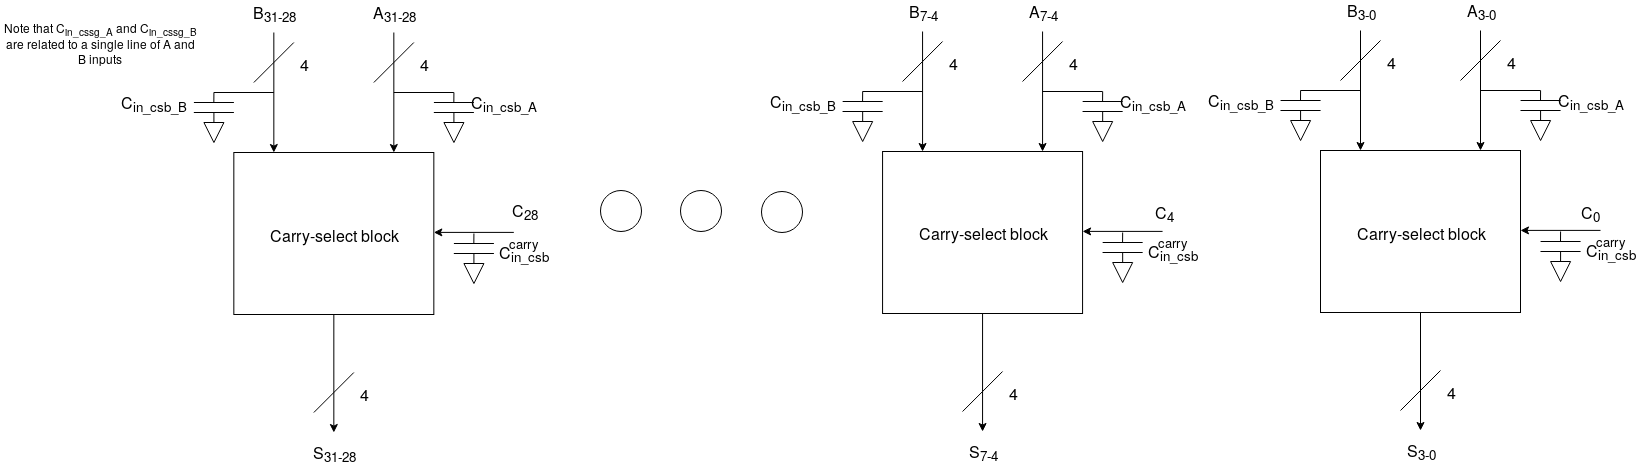
\includegraphics[width = 14 cm, height = 6 cm]{pentium/carry_select_sum_generator_schematic.png}
\caption{Carry-select sum generator schematic}
\label{fig:cssg_schematic}
\end{figure}

\begin{figure}[H]
\centering
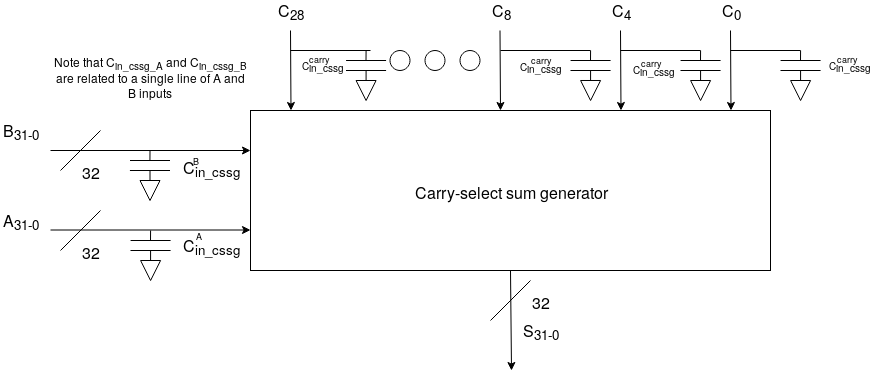
\includegraphics[width = 10 cm, height = 6 cm]{pentium/carry_select_sum_generator_black_box.png}
\caption{Carry-select sum generator black-box}
\label{fig:cssg_bb}
\end{figure}

Introducing $N$, which is the number of bits of the adder, the area can be derived:

\begin{equation}
A_{cssg} = \frac{N}{4} A_{csb}
\end{equation}

Note that the values of $N$ considered are 8, 12, 16, 20, 24, 28 and 32.

The leakage current is:
\begin{equation}
I_{leak_{cssg}} = \frac{N}{4} I_{leak_{csb}}
\end{equation}

The static power is:

\begin{equation}
P_{stat_{cssg}} = V_{DD} I_{leak_{cssg}}
\end{equation}

The dynamic power is:

\begin{equation}
P_{dyn_{cssg}} = \frac{N}{4} P_{dyn_{csb}}
\end{equation}

The intrinsic delay (the delay without load) is:
\begin{equation}
\tau_{int_{cssg}} = \tau_{int_{csb}}
\end{equation}

The $\alpha$ parameter is:
\begin{equation}
\alpha_{cssg} = \alpha_{csb}
\end{equation}

The input capacitances for each line of the A and B inputs are:
\begin{equation}
C_{in_{cssg}}^{input} = C_{in_{cssg}}^{A} = C_{in_{cssg}}^{B} = C_{in_{csb}}^{input}
\end{equation}
while the input capacitance seen from each carry input is:

\begin{equation}
C_{in_{cssg}}^{carry} = C_{in_{csb}}^{carry}
\end{equation}





\subsection{Carry-merge sparse tree}
In this subsection the three blocks that constitute the carry-merge sparse tree are presented. They are the pre-computation block (pcb), the propagate-generate block (pg) and the G-block (gb). Using these blocks the carry-merge sparse tree can be designed.





\subsubsection{Pre-computation block}
In figure \ref{pcb} it is shown the symbol and the schematic view of the pre-computation block.

\begin{figure}[H]
\centering
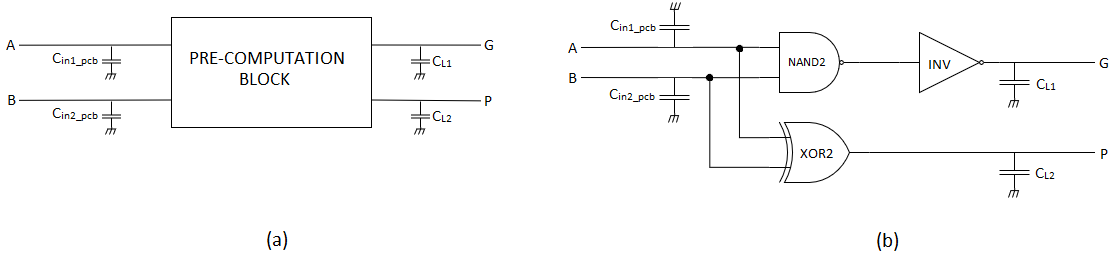
\includegraphics[width = 14cm]{pentium/pcb.png}
\caption{Pre-computation block. (a) Symbol. (b) Schematic view. }
\label{pcb}
\end{figure}

The  area of the pre-computation block is given by:
\begin{equation}
A_{pcb}=A_{nand2}+A_{inv}+A_{xor2}
\end{equation}
The leakage current is:
\begin{equation}
I_{leak_{pcb}}=I_{leak_{nand2}}+I_{leak_{inv}}+I_{leak_{xor2}}
\end{equation}
The static power is:
\begin{equation}
P_{stat_{pcb}}=V_{DD}\cdot I_{leak_{pcb}}
\end{equation}
The dynamic power is:
\begin{equation}
P_{dyn_{pcb}}=V_{DD}^2f_{CLK}E_{sw}C_{in_{inv}}
\end{equation}

The intrinsic delay (the delay without load) of the output $G$ is:
\begin{equation}
\tau_{int_{pcb_{G}}} = \tau_{int_{nand2}}+\alpha_{nand2}C_{in_{inv}}+\tau_{int_{inv}}
\end{equation}

Then the $\alpha$ parameter is:
\begin{equation}
\alpha_{pcb_{G}}=\alpha_{inv}
\end{equation}

Thus the total delay of $G$ (considering the load) is $\tau_{int_{pcb_{G}}}+\alpha_{pcb_{G}}C_{L1}$.\\\\

Analogously for the output $P$ we have:
\begin{equation}
\tau_{int_{pcb_{P}}} = \tau_{int_{xor2}}
\end{equation}

\begin{equation}
\alpha_{pcb_{P}}=\alpha_{xor2}
\end{equation}

The delay of $P$ considering the load will be $\tau_{int_{pcb_{P}}}+\alpha_{pcb_{P}}C_{L2}$.\\\\

The input capacitances of the pre-computation block are:
\begin{equation}
C_{in_{pcb}}=C_{in1_{pcb}}=C_{in2_{pcb}}=C_{in_{nand2}}+C_{in_{xor2}}
\end{equation}





\subsubsection{Propagate-generate block}
Figure \ref{fig:pg_block_schematic} shows the propagate-generate block (pg-block) schematic and figure \ref{fig:pg_bb} its black-box model.

\begin{figure}[H]
\centering
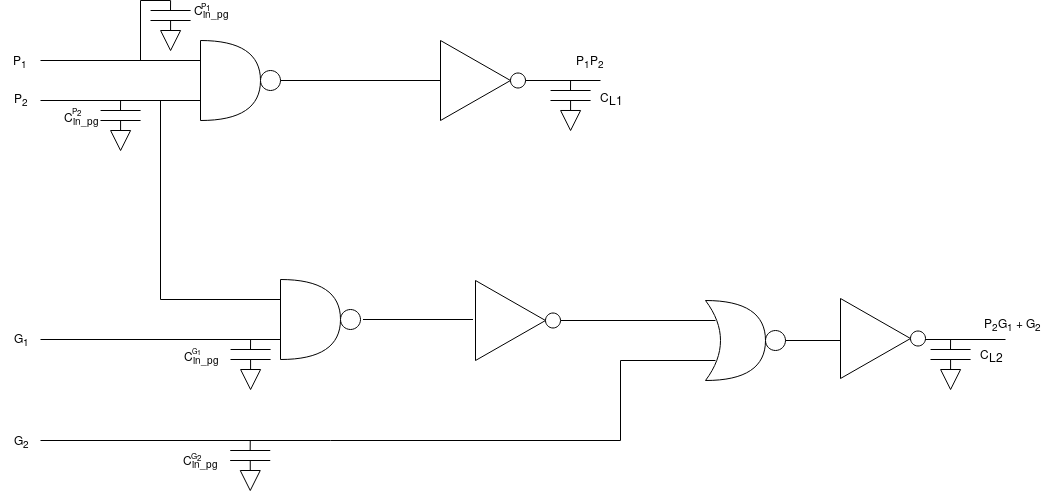
\includegraphics[width = \textwidth]{pentium/propagate_generate_block_schematic.png}
\caption{Schematic of propagate and generate carry block}
\label{fig:pg_block_schematic}
\end{figure}

\begin{figure}[H]
\centering
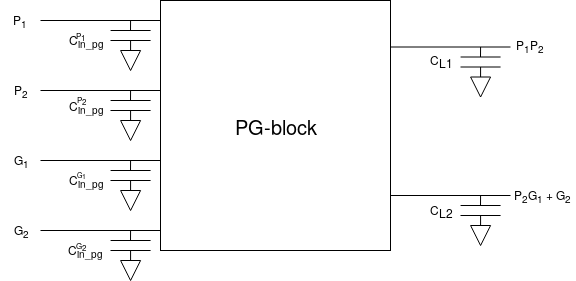
\includegraphics[width = 8 cm]{pentium/propagate_generate_block_black_box.png}
\caption{Symbol of propagate and generate carry block}
\label{fig:pg_bb}
\end{figure}

From the schematic figure, the area can be evaluated as:
\begin{equation}
A_{pg} = 2 A_{nand2} + A_{nor2} + 3 A_{inv}
\end{equation}

The leakage current is:
\begin{equation}
I_{leak_{pg}} = 2 I_{leak_{nand2}} + I_{leak_{nor2}} + 3 I_{leak_{inv}}
\end{equation}

The static power is:
\begin{equation}
P_{stat_{pg}} = V_{DD} I_{leak_{pg}}
\end{equation}

The dynamic power is:
\begin{equation}
P_{dyn_{pg}} = V_{DD}^2 f_{CLK} E_{sw} (3 C_{in_{inv}}  +  C_{in_{nor2}})
\end{equation}

The intrinsic delay (delay without load) for the $P_1 P_2$ output is:
\begin{equation}
\tau_{int_{pg_p}} = \tau_{int_{nand2}} + \alpha_{nand2} C_{in_{inv}} + \tau_{int_{inv}}
\end{equation}
The $\alpha$ parameter is:
\begin{equation}
\alpha_{pg_p} = \alpha_{inv}
\end{equation}
Thus the overall delay for the $P_1 P_2$ output  is $\tau_{int_{pg_p}} + \alpha_{pg_p} C_{L1}$.\\


The intrinsic delay for the $P_2G_1+G_2$  output is:
\begin{equation}
\tau_{int_{pg_g}} = \tau_{int_{nand2}} + \alpha_{nand2} C_{in_{inv}} + \tau_{int_{inv}} + \alpha_{inv} C_{in_{nor2}} + \tau_{int_{nor2}} + \alpha_{nor2} C_{in_{inv}} + \tau_{int_{inv}}
\end{equation}
The $\alpha$ parameter is:
\begin{equation}
\alpha_{pg_g} = \alpha_{inv}
\end{equation}
The overall delay of this output is $ \tau_{int_{pg_g}} + \alpha_{pg_g} C_{L2}$.\\

In order from $P_1$ to $G_2$, the input capacitances are:
\begin{equation}
C_{in_{pg}}^{P_1} = C_{in_{nand2}}
\end{equation}

\begin{equation}
C_{in_{pg}}^{P_2} = 2 C_{in_{nand2}}
\end{equation}

\begin{equation}
C_{in_{pg}}^{G_1} = C_{in_{nand2}}
\end{equation}

\begin{equation}
C_{in_{pg}}^{G_2} = C_{in_{nor2}}
\end{equation}

Then the total input capacitance for this block is defined as:
\begin{equation}
C_{in_{pg}}^{tot} = C_{in_{pg}}^{P_1} + C_{in_{pg}}^{P_2} + C_{in_{pg}}^{G_1} + C_{in_{pg}}^{G_2}
\end{equation}





\subsubsection{G-block}
This block is the same of the previous one but there is only the second output (G-output). In figure \ref{gb} it is shown the symbol and the schematic view of the G-block.

\begin{figure}[H]
\centering
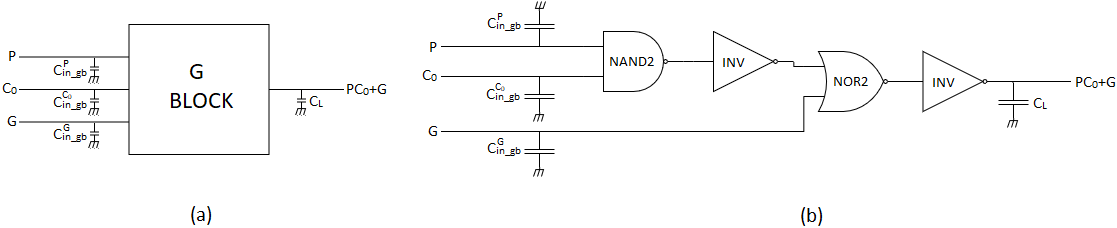
\includegraphics[width = 14cm]{pentium/gb.png}
\caption{G-block. (a) Symbol. (b) Schematic view. }
\label{gb}
\end{figure}

The  area of the G-block is given by:
\begin{equation}
A_{gb}=A_{nand2}+A_{nor2}+2A_{inv}
\end{equation}
The leakage current is:
\begin{equation}
I_{leak_{gb}}=I_{leak_{nand2}}+I_{leak_{nor2}}+2I_{leak_{inv}}
\end{equation}
The static power is:
\begin{equation}
P_{stat_{gb}}=V_{DD}\cdot I_{leak_{gb}}
\end{equation}
The dynamic power is:
\begin{equation}
P_{dyn_{gb}}=V_{DD}^2f_{CLK}E_{sw}(2C_{in_{inv}}+C_{in_{nor2}})
\end{equation}

The intrinsic delay (the delay without load) is:
\begin{equation}
\tau_{int_{gb}} = \tau_{int_{nand2}} + \alpha_{nand2} C_{in_{inv}} + \tau_{int_{inv}} + \alpha_{inv} C_{in_{nor2}} + \tau_{int_{nor2}} + \alpha_{nor2} C_{in_{inv}} + \tau_{int_{inv}}
\end{equation}

Then the $\alpha$ parameter is:
\begin{equation}
\alpha_{gb}=\alpha_{inv}
\end{equation}

Thus the total delay (considering the load) is $\tau_{int_{gb}}+\alpha_{gb}C_{L}$.\\\\
The input capacitances are:
\begin{equation}
C_{in_{gb}}^{P} = C_{in_{nand2}}
\end{equation}
\begin{equation}
C_{in_{gb}}^{C_0} = C_{in_{nand2}}
\end{equation}
\begin{equation}
C_{in_{gb}}^{G} = C_{in_{nor2}}
\end{equation}





\subsubsection{Carry-merge sparse tree}
In Figure \ref{tree_black_box} and in Figure \ref{tree_interno} are respectively shown the black-box and the schematic view of the carry-merge sparse tree for a number of bit $N=32$.

\begin{figure}[H]
\centering
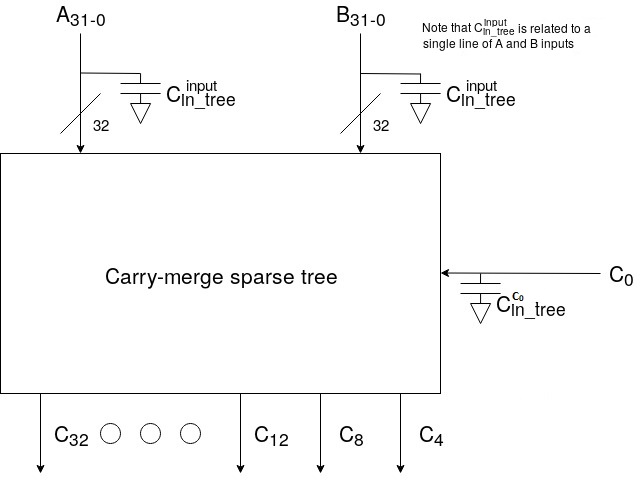
\includegraphics[width = 8cm]{pentium/tree_black_box.jpeg}
\caption{Symbol of carry-merge sparse tree with 32 bit}
\label{tree_black_box}
\end{figure}

\begin{figure}[H]
\centering
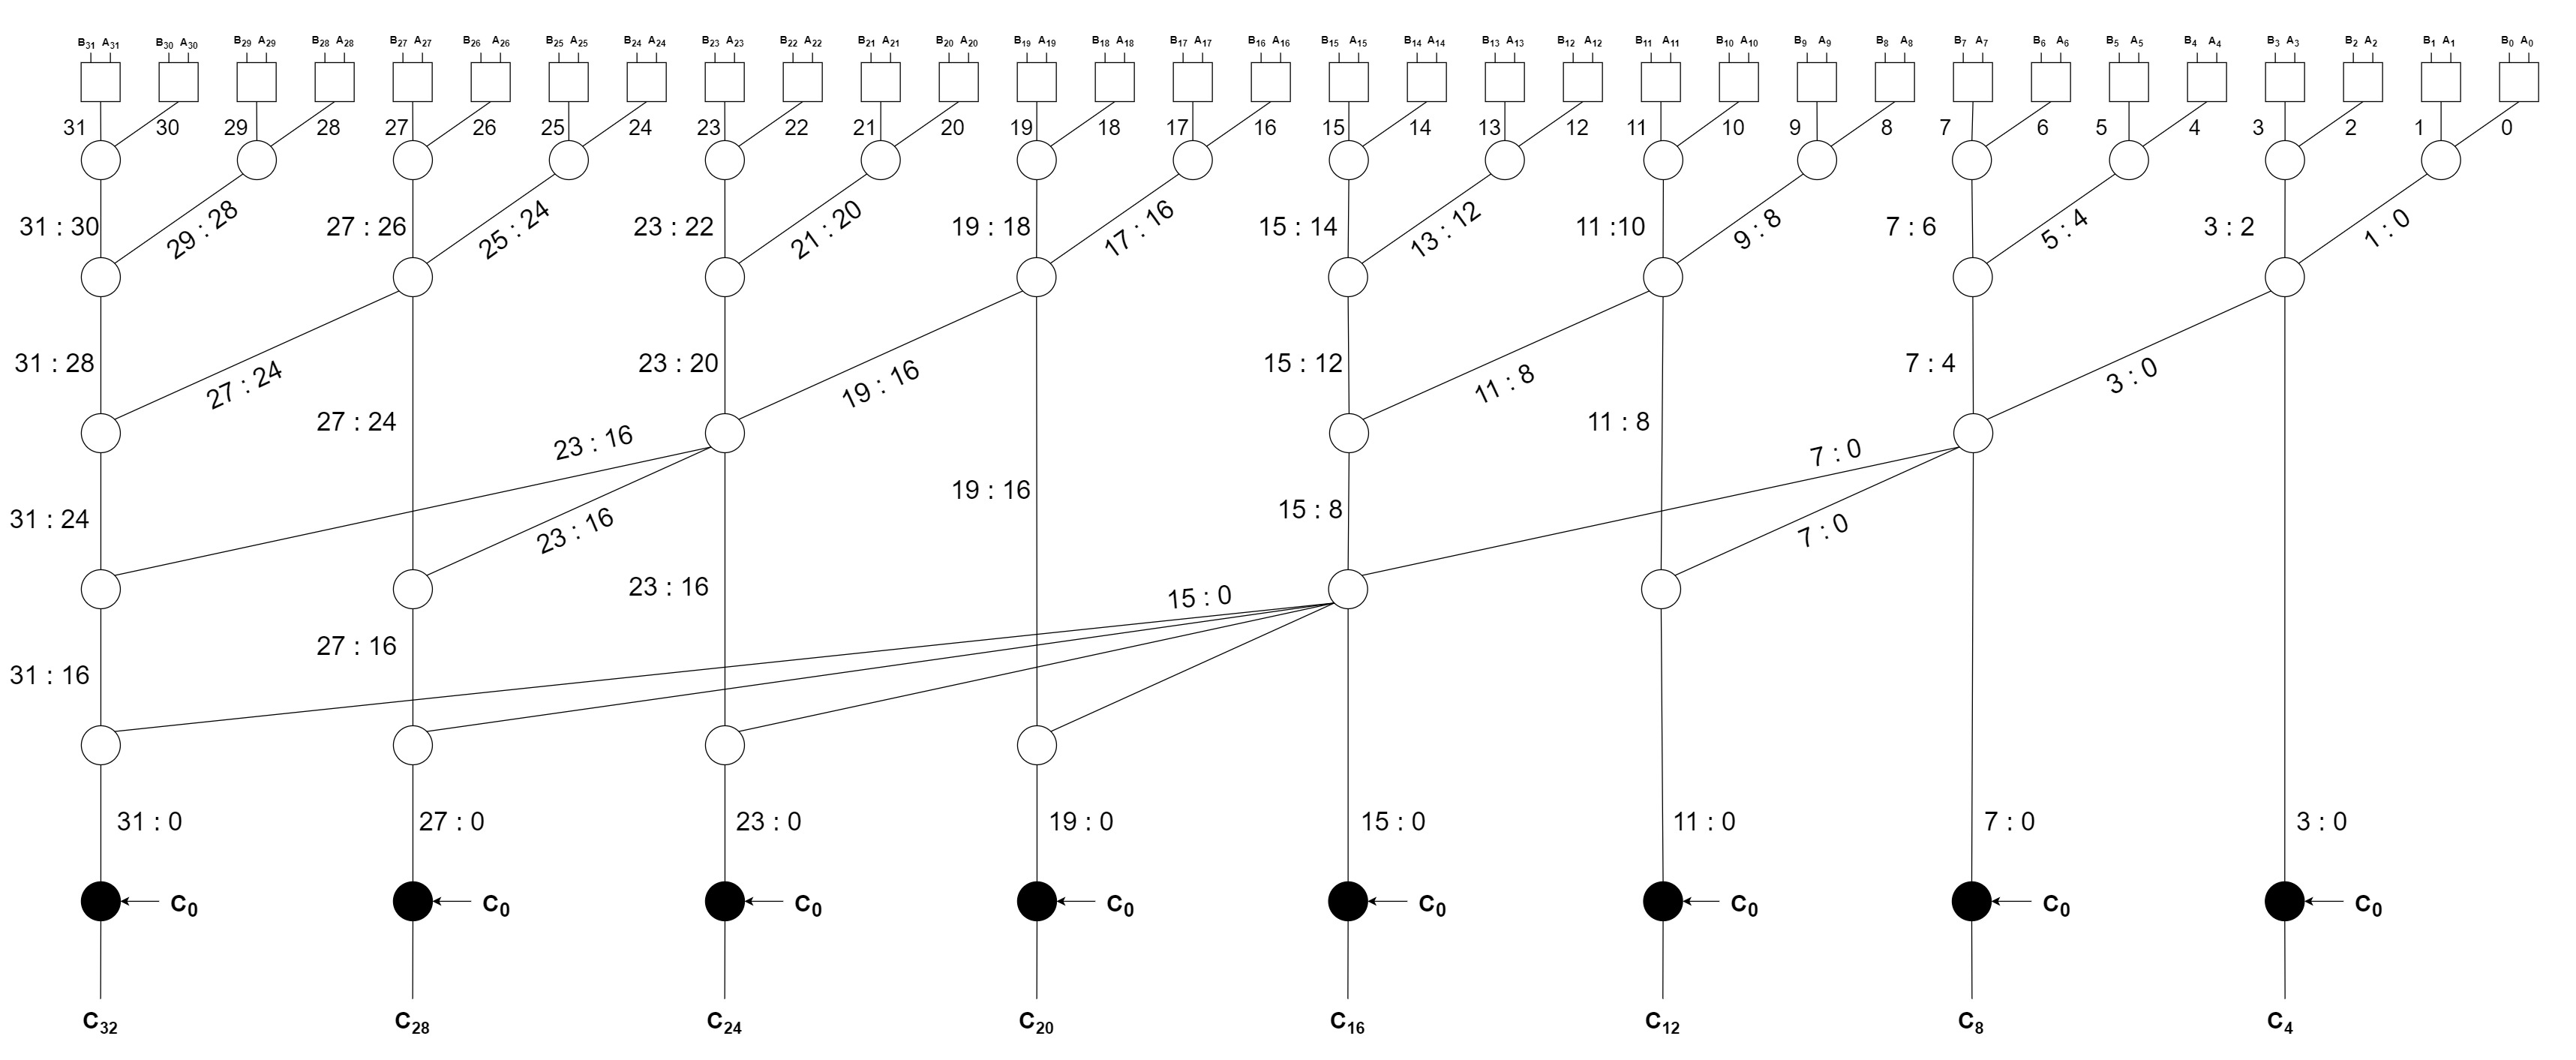
\includegraphics[width = 14cm]{pentium/tree_interno.jpg}
\caption{Schematic view of the carry-merge sparse tree with 32 bit}
\label{tree_interno}
\end{figure}

In the schematic view the white squares are pre-computation blocks (pcb), the white circles are propagate-generate blocks (pg) and the black circles are G-blocks (gb). Note that the pcb and pg-blocks have two output but in the schematic view there is only one line for both of them. This is only to have a less complicated picture of the schematic view.\\
The outputs of this tree are the carry from $C_4$ to $C_{32}$ with a step of 4.\\
Area, power consumption and delay of the tree are evaluated as a function of the number of bit $N$, in the case where $N$ can be equal to 8, 12, 16, 20, 24, 28 or 32.\\
The area of the tree is equal to:
\begin{equation}
A_{tree} = N_{pcb}A_{pcb}+N_{pg}A_{pg}+N_{gb}A_{gb}
\end{equation}

Where:
\begin{equation}
N_{pcb}=N
\end{equation}
and
\begin{equation}
N_{gb}=\frac{N}{4}
\end{equation}
$N_{pg}$ cannot be written as a function of $N$ in a simple way. Therefore the number of pg-blocks for each case looking at the figure \ref{tree_interno} can be counted.
\begin{equation}
N_{pg}=
   \begin{cases}
   7 \,\,\,\,\,\,\,\,\,\,\,\,\,\, N=8 \\
   11 \,\,\,\,\,\,\,\,\,\,\, N=12 \\
   16 \,\,\,\,\,\,\,\,\,\,\, N=16 \\
   20 \,\,\,\,\,\,\,\,\,\,\, N=20 \\
   25 \,\,\,\,\,\,\,\,\,\,\, N=24 \\
   30 \,\,\,\,\,\,\,\,\,\,\, N=28 \\
   36 \,\,\,\,\,\,\,\,\,\,\, N=32 \\
   \end{cases}
\end{equation}


The leakage current is given by:
\begin{equation}
I_{leak_{tree}}=N_{pcb}I_{leak_{pcb}}+N_{pg}I_{leak_{pg}}+N_{gb}I_{leak_{gb}}
\end{equation}
The static power is:
\begin{equation}
P_{stat_{tree}}=V_{DD}\cdot I_{leak_{tree}}
\end{equation}
The dynamic power is:
\begin{equation}
P_{dyn_{tree}} = V_{DD}^2 f_{CLK} E_{sw} \Bigl[N_{pg}C_{in_{pg}}^{tot} + N_{gb}\bigl( C_{in_{gb}}^{P}+ C_{in_{gb}}^{G} \bigr)\Bigr] + N_{pcb} P_{dyn_{pcb}} + N_{pg} P_{pyn_{pg}} + N_{gb} P_{dyn_{gb}}
\end{equation}

Without doing simplifications (for instance considering an upper bound for the delay instead of the real delay), there is not a simple way to evaluate the delay of the tree as a function of $N$. This is why when $N$ changes, the capacitances in the nodes of the tree can change.\\
To evaluate the delay of the tree no simplifications are used. For this reason, each case of $N$ is considered separately.\\\\
First of all, we note that the pcb-blocks have always the same load for each value of $N$. Thus we can compute the total delay of a pcb-block as:
\begin{equation}
\tau_{pcb_{tree}} = max\Bigl(\tau_{pcb_{tree}}^G, \tau_{pcb_{tree}}^P\Bigr)
\end{equation}
where $\tau_{pcb_{tree}}^G$ is the delay related to the $G$ output while $\tau_{pcb_{tree}}^P$ is related to the $P$ one. Since the load of each the pcb-block is always one pg-block, it can be written:
\begin{equation}
\tau_{pcb_{tree}}^G = \tau_{int_{pcb_{G}}} +  \alpha_{pcb_{G}} \cdot max\Bigl(C_{in_{pg}}^{G_1}, C_{in_{pg}}^{G_2} \Bigr)
\end{equation}
\begin{equation}
\tau_{pcb_{tree}}^P = \tau_{int_{pcb_{P}}} +  \alpha_{pcb_{P}} \cdot max\Bigl(C_{in_{pg}}^{P_1}, C_{in_{pg}}^{P_2} \Bigr)
\end{equation}

In order to compute the delay of the tree for each value of $N$, it is useful computing the delay of the pg-block for different loads. \\
$\tau_{pg_{xy}}^G$ is the delay related to the output $G$ of a pg-block  when the load is a number $x$ of pg-blocks and a number $y$ of G-blocks. Similarly $\tau_{pg_{xy}}^P$ is the delay related to the output $P$ of a pg-block  when the load is a number $x$ of pg-blocks and a number $y$ of G-blocks.\\

Thus the delay of a pg-block with a load of 1 pg-block and 0 G-block is:
\begin{equation}
\tau_{pg_{10}} = max\Bigl( \tau_{pg_{10}}^G, \tau_{pg_{10}}^P \Bigr)
\end{equation}
 where:
\begin{equation}
\tau_{pg_{10}}^G = \tau_{int_{pg_g}} + \alpha_{pg_g} \cdot max\Bigl( C_{in_{pg}}^{G_1}, C_{in_{pg}}^{G_2}  \Bigr)
\end{equation}
\begin{equation}
\tau_{pg_{10}}^P = \tau_{int_{pg_p}} + \alpha_{pg_p} \cdot max\Bigl( C_{in_{pg}}^{P_1}, C_{in_{pg}}^{P_2}  \Bigr)
\end{equation}
\\
The delay of a pg-block with a load of 1 pg-block and 1 G-block is:
\begin{equation}
\tau_{pg_{11}} = max\Bigl( \tau_{pg_{11}}^G, \tau_{pg_{11}}^P \Bigr)
\end{equation}
 where:
\begin{equation}
\tau_{pg_{11}}^G = \tau_{int_{pg_g}} + \alpha_{pg_g} \cdot \Bigl[ max\Bigl( C_{in_{pg}}^{G_1}, C_{in_{pg}}^{G_2}  \Bigr) + C_{in_{gb}}^{G} \Bigr]
\end{equation}
\begin{equation}
\tau_{pg_{11}}^P = \tau_{int_{pg_p}} + \alpha_{pg_p} \cdot \Bigl[ max\Bigl( C_{in_{pg}}^{P_1}, C_{in_{pg}}^{P_2}  \Bigr) + C_{in_{gb}}^{P} \Bigr]
\end{equation}
\\
The delay of a pg-block with a load of 2 pg-block and 1 G-block is:
\begin{equation}
\tau_{pg_{21}} = max\Bigl( \tau_{pg_{21}}^G, \tau_{pg_{21}}^P \Bigr)
\end{equation}
 where:
\begin{equation}
\tau_{pg_{21}}^G = \tau_{int_{pg_g}} + \alpha_{pg_g} \cdot \Bigl[ 2max\Bigl( C_{in_{pg}}^{G_1}, C_{in_{pg}}^{G_2}  \Bigr) + C_{in_{gb}}^{G} \Bigr]
\end{equation}
\begin{equation}
\tau_{pg_{21}}^P = \tau_{int_{pg_p}} + \alpha_{pg_p} \cdot \Bigl[ 2max\Bigl( C_{in_{pg}}^{P_1}, C_{in_{pg}}^{P_2}  \Bigr) + C_{in_{gb}}^{P} \Bigr]
\end{equation}
\\
The delay of a pg-block with a load of 4 pg-block and 1 G-block is:
\begin{equation}
\tau_{pg_{41}} = max\Bigl( \tau_{pg_{41}}^G, \tau_{pg_{41}}^P \Bigr)
\end{equation}
 where:
\begin{equation}
\tau_{pg_{41}}^G = \tau_{int_{pg_g}} + \alpha_{pg_g} \cdot \Bigl[ 4max\Bigl( C_{in_{pg}}^{G_1}, C_{in_{pg}}^{G_2}  \Bigr) + C_{in_{gb}}^{G} \Bigr]
\end{equation}
\begin{equation}
\tau_{pg_{41}}^P = \tau_{int_{pg_p}} + \alpha_{pg_p} \cdot \Bigl[ 4max\Bigl( C_{in_{pg}}^{P_1}, C_{in_{pg}}^{P_2}  \Bigr) + C_{in_{gb}}^{P} \Bigr]
\end{equation}
\\
The delay of a pg-block with a load of 0 pg-block and 1 G-block is:
\begin{equation}
\tau_{pg_{01}} = max\Bigl( \tau_{pg_{01}}^G, \tau_{pg_{01}}^P \Bigr)
\end{equation}
 where:
\begin{equation}
\tau_{pg_{01}}^G = \tau_{int_{pg_g}} + \alpha_{pg_g} \cdot C_{in_{gb}}^{G}
\end{equation}
\begin{equation}
\tau_{pg_{01}}^P = \tau_{int_{pg_p}} + \alpha_{pg_p} \cdot C_{in_{gb}}^{P}
\end{equation}
\\
Now the intrinsic delay (the delay without load) of the tree, for each value of $N$, can be evaluated. We will denote the intrinsic delay as $\tau_{int_{tree}}^N$ where $N$ is the number of bit. Looking at the figure \ref{tree_interno} we can write:

\begin{equation}
\tau_{int_{tree}}^{8} = \tau_{pcb_{tree}} + \tau_{pg_{10}} + \tau_{pg_{11}} + \tau_{pg_{01}} + \tau_{int_{gb}}
\end{equation}
\begin{equation}
\tau_{int_{tree}}^{12} =  \tau_{pcb_{tree}} + \tau_{pg_{10}} + \tau_{pg_{11}} + \tau_{pg_{21}} + \tau_{pg_{01}} + \tau_{int_{gb}}
\end{equation}

\begin{equation}
\tau_{int_{tree}}^{16} = \tau_{int_{tree}}^{12}
\label{yeah1}
\end{equation}

\begin{equation}
\tau_{int_{tree}}^{20} = \tau_{pcb_{tree}} + \tau_{pg_{10}} + \tau_{pg_{11}} + \tau_{pg_{21}} + \tau_{pg_{41}} + \tau_{int_{gb}}
\end{equation}

\begin{equation}
\tau_{int_{tree}}^{24} = \tau_{int_{tree}}^{28} = \tau_{int_{tree}}^{32} = \tau_{int_{tree}}^{20}
\label{yeah2}
\end{equation}

The $\alpha$ coefficient of the tree does not depend on $N$ and it is equal to:
\begin{equation}
\alpha_{tree} = \alpha_{gb}
\end{equation}

The input capacitance for each line of the $A_{31-0}$ and $B_{31-0}$ inputs is:
\begin{equation}
C_{in_{tree}}^{input} = C_{in_{pcb}}
\end{equation}
while the input capacitance seen from the $C_0$:
\begin{equation}
C_{in_{tree}}^{C_0} = N_{gb}C_{in_{gb}}^{C_0}
\end{equation}





\subsection{Pentium IV adder}
The overall architecture can be summarized into the schematic in figure \ref{fig:pentium32adder_schematic}. The black-box symbol is reported in figure \ref{fig:pentium32adder_bb}.

\begin{figure}[H]
\centering
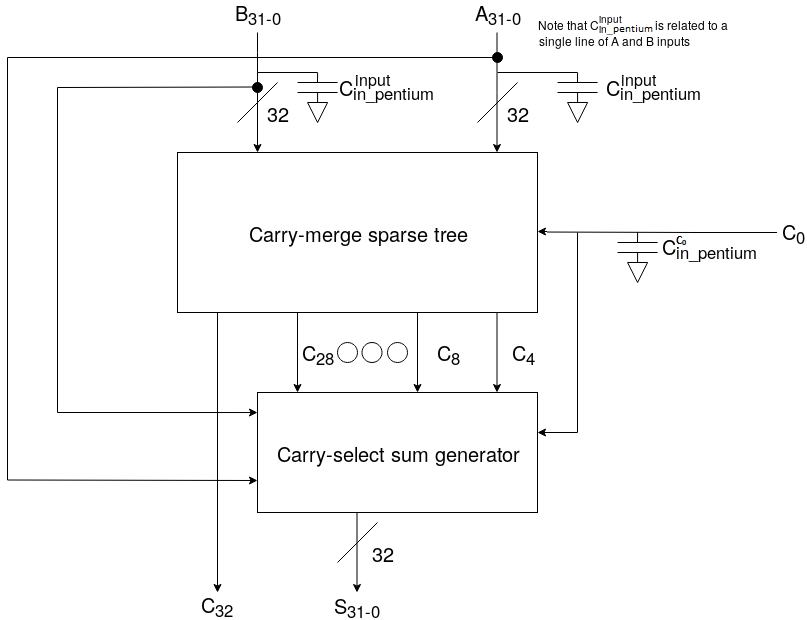
\includegraphics[width = 10 cm]{pentium/pentium32schematic.png}
\caption{Schematic of the 32-bit Pentium IV adder}
\label{fig:pentium32adder_schematic}
\end{figure}

\begin{figure}[H]
\centering
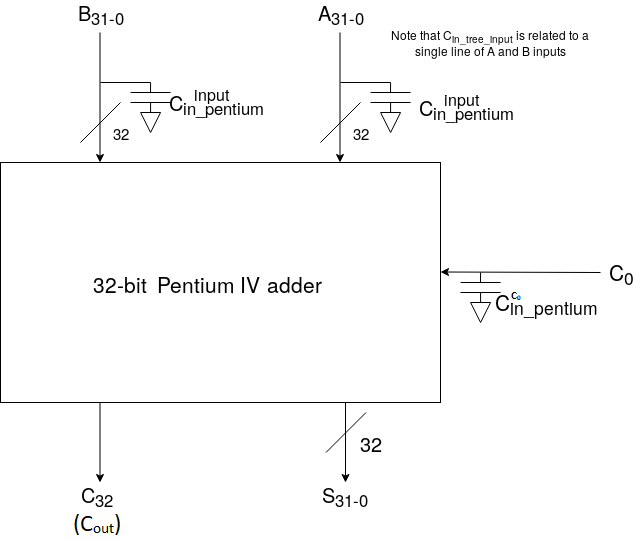
\includegraphics[width = 8 cm]{pentium/pentium32black_box.png}
\caption{Pentium IV black-box view}
\label{fig:pentium32adder_bb}
\end{figure}

The area can be evaluated as:
\begin{equation}
A_{pentium} = A_{tree} + A_{cssg}
\end{equation}

The leakage current is:
\begin{equation}
I_{leak_{pentium}} = I_{leak_{tree}} + I_{leak_{cssg}}
\end{equation}

The static power is:
\begin{equation}
P_{stat_{pentium}} = V_{DD} I_{leak_{pentium}}
\end{equation}

The dynamic power is:
\begin{equation}
P_{dyn_{pentium}} = V_{DD}^2 f_{CLK} E_{sw} \Biggl(\frac{N}{4} - 1\Biggr)C_{in_{cssg}}^{carry} + P_{dyn_{tree}} + P_{dyn_{cssg}}
\end{equation}

The input signals $A_{31-0}$ and $B_{31-0}$ enter both in the tree and in the carry-select sum generator. Thus the tree and all RCA4s inside the carry-select sum generator work in parallel. This means that if the delay of the tree ($\tau_{int_{tree}}^{N}+\alpha_{tree}C_{in_{cssg}}^{carry}$) is greater than the delay of the RCA4 ($\tau_{int_{RCA4}} + \alpha_{RCA4} C_{in_{4-mux}}^{input}$), the delay of the Pentium without load will be $\tau_{int_{tree}}^{N}+\alpha_{tree}C_{in_{cssg}}^{carry}+\tau_{int_{4-mux}}$ where $C_{in_{cssg}}^{carry} = C_{in_{csb}}^{carry}$. On the contrary, if the delay of the tree is smaller than the delay of the RCA4 (usually this case does not happen if the number of bit is big), the delay of the the Pentium without load will be $\tau_{int_{cssg}} = \tau_{int_{csb}} = \tau_{int_{RCA4}} + \alpha_{RCA4} C_{in_{4-mux}}^{input} + \tau_{int_{4-mux}}$.\\\\
Therefore the delay of the Pentium without is:
\begin{equation}
\tau_{int_{pentium}} = max \Bigl( \tau_{int_{tree}}^{N} + \alpha_{tree} C_{in_{cssg}}^{carry} + \tau_{int_{4-mux}}, \tau_{int_{cssg}} \Bigr)
\end{equation}

The $\alpha$ parameter is:
\begin{equation}
\alpha_{pentium} = \alpha_{cssg}
\end{equation}

The input capacitance for each line of the $A_{31-0}$ and $B_{31-0}$ inputs is:
\begin{equation}
C_{in_{pentium}}^{input} = C_{in_{tree}}^{input} + C_{in_{cssg}}^{input}
\end{equation}
while the input capacitance seen from the $C_0$:
\begin{equation}
C_{in_{pentium}}^{C_0} = C_{in_{tree}}^{C_0} + C_{in_{cssg}}^{carry}
\end{equation}
\\
Now the working frequency can be estimated. As already said in section \ref{ciao}, the inverse of the delay of the Pentium IV without load is used as working frequency.\\
\begin{equation}
f_{CLK} = \frac{1}{\tau_{int_{pentium}}}
\end{equation}





\section{Matlab implementation}
All the formulas in this report have been implemented in Matlab in order to evaluate area, power consumption and delay of the Pentium IV adder. Obviously the values of the input parameters described in Table \ref{library_logic_gates} are set to see the results, but  the characterization these logic gates is assumed already done by other works. For this reason reasonable values for the input parameters, considering the internal structure of the logic CMOS gates, have been used.\\
In the following is reported the Matlab code.

\lstinputlisting{pentium/Pentium_IV2.m}





\section{Results}
In this section are reported in graphs the results obtained for area, power and delay of the Pentium IV considering 8, 12, 16, 20, 24, 28 and 32 bits parallelism.\\
As expected the area increases by increasing the number of bits (figure \ref{result_area}). The static power increases with the same trend of the area (figure \ref{result_Pstat}). This is why each block in the Pentium IV has a leakage current, thus if the area increases also the static power increases.\\
If the area increases ($N$ increases), it is expected also that the dynamic power increases as it can be seen in figure \ref{result_Pdyn}.\\
Figure \ref{result_delay} shows the delay without load of the Pentium IV. It is possible to notice how the delay follows instead a different trend: this can be explained remembering that for $N=12$ and $N=16$ the tree has the exact same delay (eq.\ref{yeah1}). The same happens also in the cases in which $N=20$, $N=24$, $N=28$ and $N=32$ (eq.\ref{yeah2}).





\begin{figure}[H]
\centering
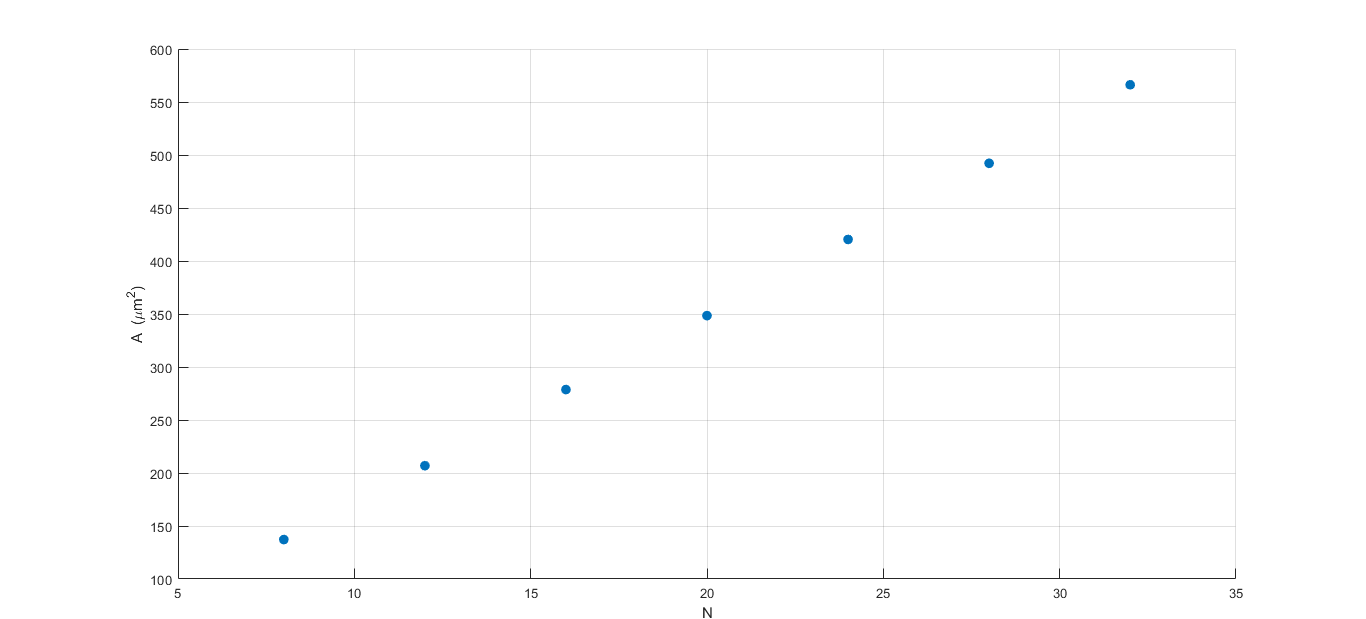
\includegraphics[width = 14 cm]{pentium/result_area.png}
\caption{Area Pentium IV as a function of $N$}
\label{result_area}
\end{figure}

\begin{figure}[H]
\centering
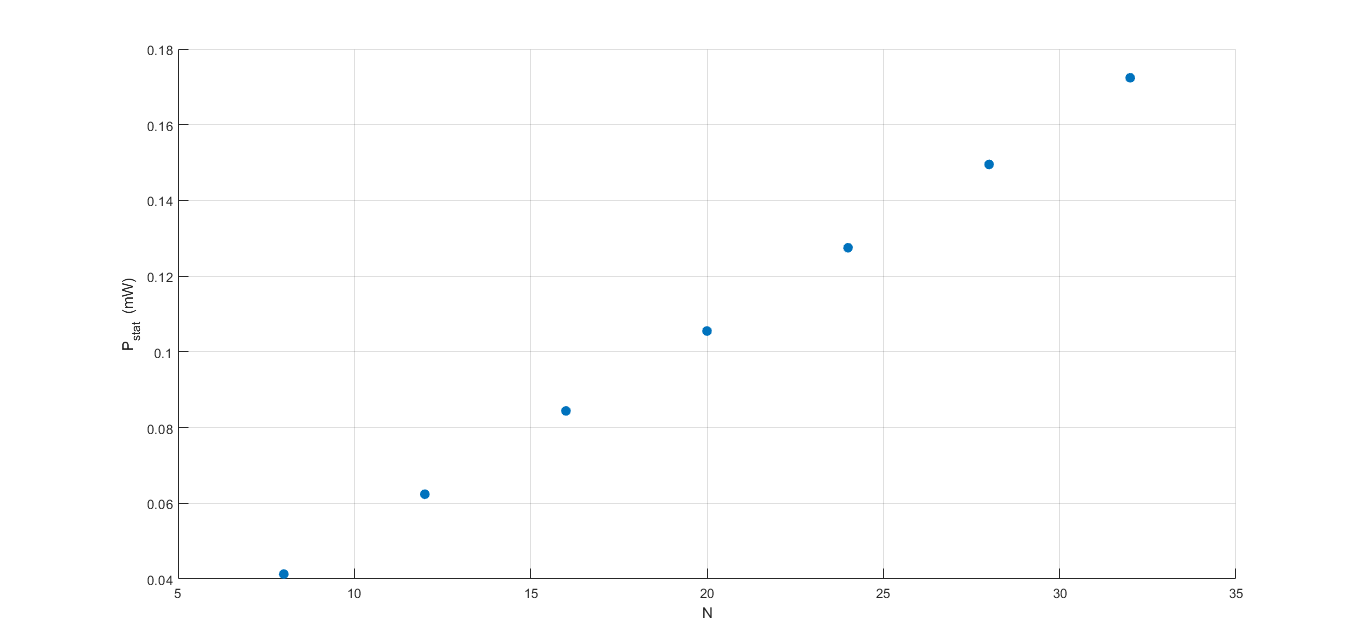
\includegraphics[width = 14 cm]{pentium/result_Pstat.png}
\caption{Static power Pentium IV as a function of $N$}
\label{result_Pstat}
\end{figure}

\begin{figure}[H]
\centering
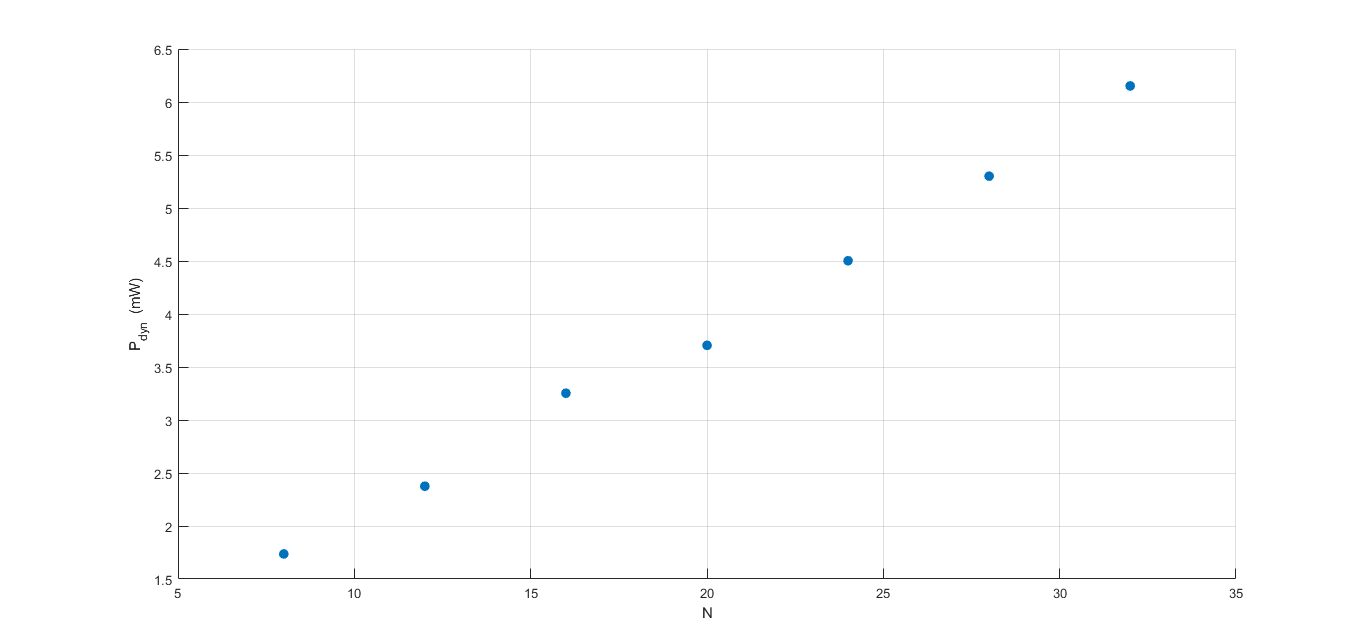
\includegraphics[width = 14 cm]{pentium/result_Pdyn.png}
\caption{Dynamic power Pentium IV as a function of $N$}
\label{result_Pdyn}
\end{figure}

\begin{figure}[H]
\centering
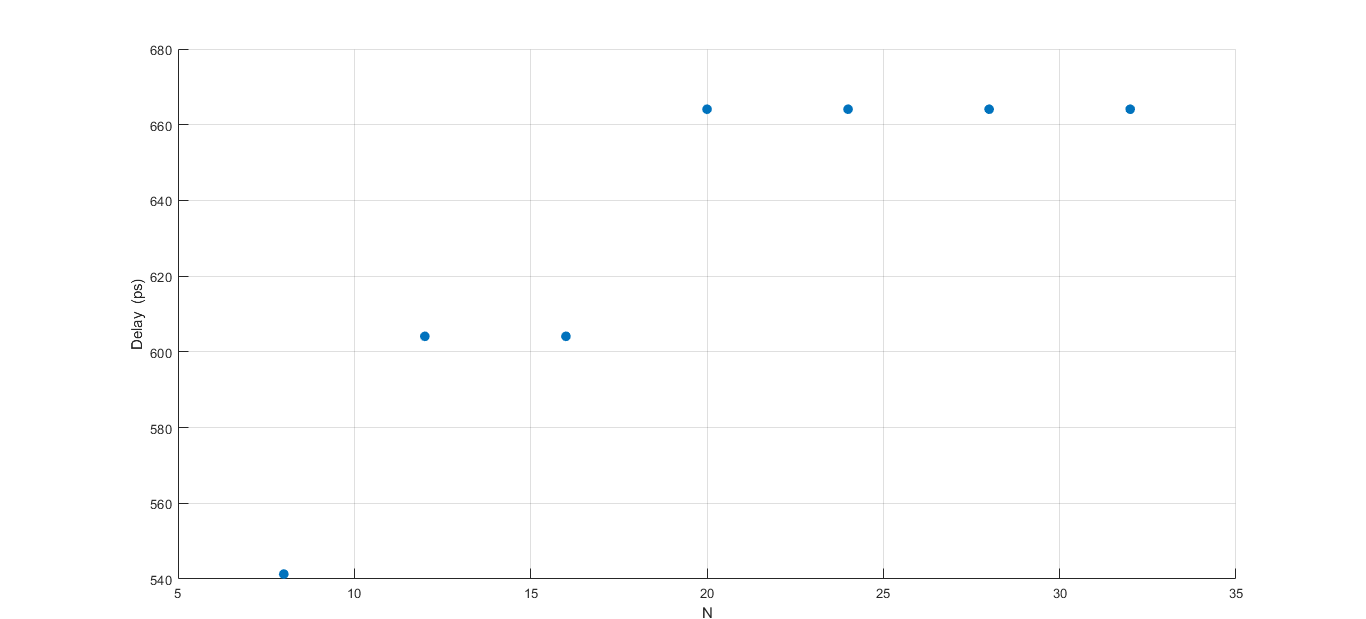
\includegraphics[width = 14 cm]{pentium/result_delay.png}
\caption{Delay without load Pentium IV as a function of $N$}
\label{result_delay}
\end{figure}



\chapter{Pipelined Wallace tree}

\section{Introduction}
The aim of this project is to implement an advanced \textbf{pipelined model} of a Wallace Tree Adder.

In particular, in the following sections, the generic structure of Wallace Tree will be described in detail and the focus will be on power consumption, occupied area and delay estimation. This particular model allows to introduce a variable number of pipeline stages along the Tree structure: the estimations will therefore take into account the pipeline structure contributions for area, power consumption and total delay.
Calculations have been performed considering, for half adders and full adders, NAND2-based structures while for D flip flops both NAND2 and INV gates.
Matlab implementation has been also reported.

The used technological parameters refer to \textit{Bulk Technology HP 2009}.
\section{Theoretical analysis}
\subsection{Wallace tree design}

Wallace tree is an efficient structure in which half and full adders can be arranged in order to add multiple operands. This structrure is often used in multipliers in order to sum up together the previously-computed partial products.
The main idea is to exploit a partial addition by columns.\\

The first step needed to implement a Wallace Tree Adder is to correctly align data so that partial terms with the same weight are in the same column.

At this point, the summands are grouped by three. The bits of each column are added together using a full adder or an half adder.
An HA is able to compress two bits with weight $k$ to one bit of weight $k$ and one bit of weight $k+1$. FAs does the same thing with three bits instead allowing a compression ratio equal to $1.5$. 
For this reason, starting from a structure with $n$ operands several levels of HAs and FAs are needed to compress these $n$ summands to two operands. Finally, when the tree has reduced the operands from $n$ to two, they are added together by a fast adder. \cite{Wallace}

The number of required levels $L$ and the maximum number of elements at each level can be obtained as follows.
The maximum number of elements at the last level (before the final adder) is two ($l_0=2$).

At the generic level $j$ the maximum number of elements is instead given by the following expression: 
\[
	l_j=\left\lfloor\dfrac{3}{2}l_{j-1}\right\rfloor
\]

The number of required levels can be obtained by repeating this operation until $j \ge n$.

In order to better illustrate the behaviour of the system is often used the dot notation. An example can be seen in Figure \ref{fig:wallace_tree} (this particular Figure has been generated through the Matlab code).

Wallace allocation of the adders is ASAP, this means that at each level dots are divided in three-dots-wide stripes and each stripe is filled with the maximum possible amount of FAs and HAs.
Stripes that only have one or two operands are forwarded to the next level of the tree structure.

This execution flow can also be pipelined: in particular, in this work, different Wallace tree solutions have been explored and compared in terms of pipeline depth. Positive-edge triggered D flip flops have been inserted to store the outputs of the adders (sum and carry bits). In this way the computation performed by the tree is splitted onto multiple clock cycles depending on the depth of the tree.
\subsection{Occupied Area}
In order to evaluate the occupied area of the Wallace Tree, the number of full adders, half adders and D flip flops have been considered. The adders have been implemented by using exclusively ND2 gate while flip flops also include inverter gates.

In Figures \ref{fig:half_adder}, \ref{fig:full_adder} and \ref{fig:f_f} are shown the designs of an half adder, a full adder and D flip flops implemented as previously described.

\begin{figure}[H]
	\centering
	\textsf{{\fontsize{9pt}{5.5pt}
			\begin{pgfpicture}{0cm}{0cm}{217pt}{113pt}
% Created by FidoCadJ ver. 0.24.6, export filter by Davide Bucci
\pgfsetxvec{\pgfpoint{1pt}{0pt}}
\pgfsetyvec{\pgfpoint{0pt}{1pt}}
\pgfsetroundjoin 
\pgfsetroundcap
\pgftranslateto{\pgfxy(0,113)}
\begin{pgfmagnify}{1}{-1}
% Layer color definitions
\definecolor{layer0}{rgb}{0.0,0.0,0.0}
\definecolor{layer1}{rgb}{0.0,0.0,0.5}
\definecolor{layer2}{rgb}{1.0,0.0,0.0}
\definecolor{layer3}{rgb}{0.0,0.5,0.5}
\definecolor{layer4}{rgb}{1.0,0.78,0.0}
\definecolor{layer5}{rgb}{0.5,1.0,0.0}
\definecolor{layer6}{rgb}{0.0,1.0,1.0}
\definecolor{layer7}{rgb}{0.0,0.5,0.0}
\definecolor{layer8}{rgb}{0.6,0.8,0.2}
\definecolor{layer9}{rgb}{1.0,0.08,0.58}
\definecolor{layer10}{rgb}{0.71,0.61,0.05}
\definecolor{layer11}{rgb}{0.0,0.5,1.0}
\definecolor{layer12}{rgb}{0.88,0.88,0.88}
\definecolor{layer13}{rgb}{0.64,0.64,0.64}
\definecolor{layer14}{rgb}{0.37,0.37,0.37}
\definecolor{layer15}{rgb}{0.0,0.0,0.0}
% End of color definitions
\color{layer0}
\pgfsetlinewidth{0.7pt}
\pgfline{\pgfxy(33.0,31.0)}{\pgfxy(40.0,31.0)}
\pgfline{\pgfxy(40.0,28.0)}{\pgfxy(40.0,48.0)}
\pgfline{\pgfxy(33.0,45.0)}{\pgfxy(40.0,45.0)}
\pgfline{\pgfxy(40.0,48.0)}{\pgfxy(51.0,48.0)}
\pgfline{\pgfxy(40.0,28.0)}{\pgfxy(51.0,28.0)}
\pgfmoveto{\pgfxy(51,28)} 
\pgfcurveto{\pgfxy(64,28)}{\pgfxy(64,48)}{\pgfxy(51,48)}
\pgfstroke
\pgfellipse[stroke]{\pgfxy(62.5,38.0)}{\pgfxy(1.5,0)}{\pgfxy(0,1.0)}
\pgfline{\pgfxy(64.0,38.0)}{\pgfxy(68.0,38.0)}
\pgfline{\pgfxy(82.0,10.0)}{\pgfxy(89.0,10.0)}
\pgfline{\pgfxy(89.0,7.0)}{\pgfxy(89.0,27.0)}
\pgfline{\pgfxy(82.0,24.0)}{\pgfxy(89.0,24.0)}
\pgfline{\pgfxy(89.0,27.0)}{\pgfxy(100.0,27.0)}
\pgfline{\pgfxy(89.0,7.0)}{\pgfxy(100.0,7.0)}
\pgfmoveto{\pgfxy(100,7)} 
\pgfcurveto{\pgfxy(113,7)}{\pgfxy(113,27)}{\pgfxy(100,27)}
\pgfstroke
\pgfellipse[stroke]{\pgfxy(111.5,17.0)}{\pgfxy(1.5,0)}{\pgfxy(0,1.0)}
\pgfline{\pgfxy(113.0,17.0)}{\pgfxy(117.0,17.0)}
\pgfline{\pgfxy(82.0,52.0)}{\pgfxy(89.0,52.0)}
\pgfline{\pgfxy(89.0,49.0)}{\pgfxy(89.0,69.0)}
\pgfline{\pgfxy(82.0,66.0)}{\pgfxy(89.0,66.0)}
\pgfline{\pgfxy(89.0,69.0)}{\pgfxy(100.0,69.0)}
\pgfline{\pgfxy(89.0,49.0)}{\pgfxy(100.0,49.0)}
\pgfmoveto{\pgfxy(100,49)} 
\pgfcurveto{\pgfxy(113,49)}{\pgfxy(113,69)}{\pgfxy(100,69)}
\pgfstroke
\pgfellipse[stroke]{\pgfxy(111.5,59.0)}{\pgfxy(1.5,0)}{\pgfxy(0,1.0)}
\pgfline{\pgfxy(113.0,59.0)}{\pgfxy(117.0,59.0)}
\pgfline{\pgfxy(82.0,94.0)}{\pgfxy(89.0,94.0)}
\pgfline{\pgfxy(89.0,91.0)}{\pgfxy(89.0,111.0)}
\pgfline{\pgfxy(82.0,108.0)}{\pgfxy(89.0,108.0)}
\pgfline{\pgfxy(89.0,111.0)}{\pgfxy(100.0,111.0)}
\pgfline{\pgfxy(89.0,91.0)}{\pgfxy(100.0,91.0)}
\pgfmoveto{\pgfxy(100,91)} 
\pgfcurveto{\pgfxy(113,91)}{\pgfxy(113,111)}{\pgfxy(100,111)}
\pgfstroke
\pgfellipse[stroke]{\pgfxy(111.5,101.0)}{\pgfxy(1.5,0)}{\pgfxy(0,1.0)}
\pgfline{\pgfxy(113.0,101.0)}{\pgfxy(117.0,101.0)}
\pgfline{\pgfxy(131.0,31.0)}{\pgfxy(138.0,31.0)}
\pgfline{\pgfxy(138.0,28.0)}{\pgfxy(138.0,48.0)}
\pgfline{\pgfxy(131.0,45.0)}{\pgfxy(138.0,45.0)}
\pgfline{\pgfxy(138.0,48.0)}{\pgfxy(149.0,48.0)}
\pgfline{\pgfxy(138.0,28.0)}{\pgfxy(149.0,28.0)}
\pgfmoveto{\pgfxy(149,28)} 
\pgfcurveto{\pgfxy(162,28)}{\pgfxy(162,48)}{\pgfxy(149,48)}
\pgfstroke
\pgfellipse[stroke]{\pgfxy(160.5,38.0)}{\pgfxy(1.5,0)}{\pgfxy(0,1.0)}
\pgfline{\pgfxy(162.0,38.0)}{\pgfxy(166.0,38.0)}
\pgfline{\pgfxy(68.0,38.0)}{\pgfxy(75.0,38.0)}
\pgfline{\pgfxy(75.0,38.0)}{\pgfxy(75.0,24.0)}
\pgfline{\pgfxy(75.0,24.0)}{\pgfxy(82.0,24.0)}
\pgfline{\pgfxy(75.0,38.0)}{\pgfxy(75.0,52.0)}
\pgfline{\pgfxy(75.0,52.0)}{\pgfxy(82.0,52.0)}
\pgfsetlinewidth{0.33pt}
\pgfcircle[fill]{\pgfxy(75,38)}{1.4pt}\pgfsetlinewidth{0.7pt}
\pgfline{\pgfxy(68.0,101.0)}{\pgfxy(75.0,101.0)}
\pgfline{\pgfxy(75.0,101.0)}{\pgfxy(75.0,94.0)}
\pgfline{\pgfxy(75.0,94.0)}{\pgfxy(82.0,94.0)}
\pgfline{\pgfxy(75.0,101.0)}{\pgfxy(75.0,108.0)}
\pgfline{\pgfxy(75.0,108.0)}{\pgfxy(82.0,108.0)}
\pgfsetlinewidth{0.33pt}
\pgfcircle[fill]{\pgfxy(75,101)}{1.4pt}\pgfsetlinewidth{0.7pt}
\pgfline{\pgfxy(12.0,10.0)}{\pgfxy(82.0,10.0)}
\pgfline{\pgfxy(12.0,66.0)}{\pgfxy(82.0,66.0)}
\pgfline{\pgfxy(33.0,31.0)}{\pgfxy(33.0,10.0)}
\pgfline{\pgfxy(33.0,45.0)}{\pgfxy(33.0,66.0)}
\pgfsetlinewidth{0.33pt}
\pgfcircle[fill]{\pgfxy(33,10)}{1.4pt}\pgfcircle[fill]{\pgfxy(33,66)}{1.4pt}\pgfsetlinewidth{0.7pt}
\pgfline{\pgfxy(117.0,17.0)}{\pgfxy(124.0,17.0)}
\pgfline{\pgfxy(124.0,17.0)}{\pgfxy(124.0,31.0)}
\pgfline{\pgfxy(124.0,31.0)}{\pgfxy(131.0,31.0)}
\pgfline{\pgfxy(117.0,59.0)}{\pgfxy(124.0,59.0)}
\pgfline{\pgfxy(124.0,59.0)}{\pgfxy(124.0,45.0)}
\pgfline{\pgfxy(124.0,45.0)}{\pgfxy(131.0,45.0)}
\pgfline{\pgfxy(166.0,38.0)}{\pgfxy(187.0,38.0)}
\pgfline{\pgfxy(117.0,101.0)}{\pgfxy(187.0,101.0)}
\begin{pgfmagnify}{1}{-1}
\pgfputat{\pgfxy(5,-6)}{\pgfbox[left,top]{A}}
\end{pgfmagnify}
\begin{pgfmagnify}{1}{-1}
\pgfputat{\pgfxy(5,-62)}{\pgfbox[left,top]{B}}
\end{pgfmagnify}
\begin{pgfmagnify}{1}{-1}
\pgfputat{\pgfxy(190,-34)}{\pgfbox[left,top]{Sum}}
\end{pgfmagnify}
\begin{pgfmagnify}{1}{-1}
\pgfputat{\pgfxy(190,-97)}{\pgfbox[left,top]{Carry}}
\end{pgfmagnify}
\pgfline{\pgfxy(68.0,38.0)}{\pgfxy(68.0,101.0)}
\pgfsetlinewidth{0.33pt}
\pgfcircle[fill]{\pgfxy(68,38)}{1.4pt}\end{pgfmagnify}
\end{pgfpicture}}}
	\caption{Half Adder ND2 implementation}
	\label{fig:half_adder}
\end{figure}

\begin{figure}[H]
	\centering
	\textsf{{\fontsize{9pt}{4.0pt}
			\begin{pgfpicture}{0cm}{0cm}{383pt}{141pt}
% Created by FidoCadJ ver. 0.24.6, export filter by Davide Bucci
\pgfsetxvec{\pgfpoint{1pt}{0pt}}
\pgfsetyvec{\pgfpoint{0pt}{1pt}}
\pgfsetroundjoin 
\pgfsetroundcap
\pgftranslateto{\pgfxy(0,141)}
\begin{pgfmagnify}{1}{-1}
% Layer color definitions
\definecolor{layer0}{rgb}{0.0,0.0,0.0}
\definecolor{layer1}{rgb}{0.0,0.0,0.5}
\definecolor{layer2}{rgb}{1.0,0.0,0.0}
\definecolor{layer3}{rgb}{0.0,0.5,0.5}
\definecolor{layer4}{rgb}{1.0,0.78,0.0}
\definecolor{layer5}{rgb}{0.5,1.0,0.0}
\definecolor{layer6}{rgb}{0.0,1.0,1.0}
\definecolor{layer7}{rgb}{0.0,0.5,0.0}
\definecolor{layer8}{rgb}{0.6,0.8,0.2}
\definecolor{layer9}{rgb}{1.0,0.08,0.58}
\definecolor{layer10}{rgb}{0.71,0.61,0.05}
\definecolor{layer11}{rgb}{0.0,0.5,1.0}
\definecolor{layer12}{rgb}{0.88,0.88,0.88}
\definecolor{layer13}{rgb}{0.64,0.64,0.64}
\definecolor{layer14}{rgb}{0.37,0.37,0.37}
\definecolor{layer15}{rgb}{0.0,0.0,0.0}
% End of color definitions
\color{layer0}
\pgfsetlinewidth{0.7pt}
\pgfline{\pgfxy(40.0,31.0)}{\pgfxy(47.0,31.0)}
\pgfline{\pgfxy(47.0,28.0)}{\pgfxy(47.0,48.0)}
\pgfline{\pgfxy(40.0,45.0)}{\pgfxy(47.0,45.0)}
\pgfline{\pgfxy(47.0,48.0)}{\pgfxy(58.0,48.0)}
\pgfline{\pgfxy(47.0,28.0)}{\pgfxy(58.0,28.0)}
\pgfmoveto{\pgfxy(58,28)} 
\pgfcurveto{\pgfxy(71,28)}{\pgfxy(71,48)}{\pgfxy(58,48)}
\pgfstroke
\pgfellipse[stroke]{\pgfxy(69.5,38.0)}{\pgfxy(1.5,0)}{\pgfxy(0,1.0)}
\pgfline{\pgfxy(71.0,38.0)}{\pgfxy(75.0,38.0)}
\pgfline{\pgfxy(89.0,10.0)}{\pgfxy(96.0,10.0)}
\pgfline{\pgfxy(96.0,7.0)}{\pgfxy(96.0,27.0)}
\pgfline{\pgfxy(89.0,24.0)}{\pgfxy(96.0,24.0)}
\pgfline{\pgfxy(96.0,27.0)}{\pgfxy(107.0,27.0)}
\pgfline{\pgfxy(96.0,7.0)}{\pgfxy(107.0,7.0)}
\pgfmoveto{\pgfxy(107,7)} 
\pgfcurveto{\pgfxy(120,7)}{\pgfxy(120,27)}{\pgfxy(107,27)}
\pgfstroke
\pgfellipse[stroke]{\pgfxy(118.5,17.0)}{\pgfxy(1.5,0)}{\pgfxy(0,1.0)}
\pgfline{\pgfxy(120.0,17.0)}{\pgfxy(124.0,17.0)}
\pgfline{\pgfxy(89.0,52.0)}{\pgfxy(96.0,52.0)}
\pgfline{\pgfxy(96.0,49.0)}{\pgfxy(96.0,69.0)}
\pgfline{\pgfxy(89.0,66.0)}{\pgfxy(96.0,66.0)}
\pgfline{\pgfxy(96.0,69.0)}{\pgfxy(107.0,69.0)}
\pgfline{\pgfxy(96.0,49.0)}{\pgfxy(107.0,49.0)}
\pgfmoveto{\pgfxy(107,49)} 
\pgfcurveto{\pgfxy(120,49)}{\pgfxy(120,69)}{\pgfxy(107,69)}
\pgfstroke
\pgfellipse[stroke]{\pgfxy(118.5,59.0)}{\pgfxy(1.5,0)}{\pgfxy(0,1.0)}
\pgfline{\pgfxy(120.0,59.0)}{\pgfxy(124.0,59.0)}
\pgfline{\pgfxy(138.0,31.0)}{\pgfxy(145.0,31.0)}
\pgfline{\pgfxy(145.0,28.0)}{\pgfxy(145.0,48.0)}
\pgfline{\pgfxy(138.0,45.0)}{\pgfxy(145.0,45.0)}
\pgfline{\pgfxy(145.0,48.0)}{\pgfxy(156.0,48.0)}
\pgfline{\pgfxy(145.0,28.0)}{\pgfxy(156.0,28.0)}
\pgfmoveto{\pgfxy(156,28)} 
\pgfcurveto{\pgfxy(169,28)}{\pgfxy(169,48)}{\pgfxy(156,48)}
\pgfstroke
\pgfellipse[stroke]{\pgfxy(167.5,38.0)}{\pgfxy(1.5,0)}{\pgfxy(0,1.0)}
\pgfline{\pgfxy(169.0,38.0)}{\pgfxy(173.0,38.0)}
\pgfline{\pgfxy(75.0,38.0)}{\pgfxy(82.0,38.0)}
\pgfline{\pgfxy(82.0,38.0)}{\pgfxy(82.0,24.0)}
\pgfline{\pgfxy(82.0,24.0)}{\pgfxy(89.0,24.0)}
\pgfline{\pgfxy(82.0,38.0)}{\pgfxy(82.0,52.0)}
\pgfline{\pgfxy(82.0,52.0)}{\pgfxy(89.0,52.0)}
\pgfsetlinewidth{0.33pt}
\pgfcircle[fill]{\pgfxy(82,38)}{1.4pt}\pgfsetlinewidth{0.7pt}
\pgfline{\pgfxy(19.0,10.0)}{\pgfxy(89.0,10.0)}
\pgfline{\pgfxy(19.0,66.0)}{\pgfxy(89.0,66.0)}
\pgfline{\pgfxy(40.0,31.0)}{\pgfxy(40.0,10.0)}
\pgfline{\pgfxy(40.0,45.0)}{\pgfxy(40.0,66.0)}
\pgfsetlinewidth{0.33pt}
\pgfcircle[fill]{\pgfxy(40,10)}{1.4pt}\pgfcircle[fill]{\pgfxy(40,66)}{1.4pt}\pgfsetlinewidth{0.7pt}
\pgfline{\pgfxy(124.0,17.0)}{\pgfxy(131.0,17.0)}
\pgfline{\pgfxy(131.0,17.0)}{\pgfxy(131.0,31.0)}
\pgfline{\pgfxy(131.0,31.0)}{\pgfxy(138.0,31.0)}
\pgfline{\pgfxy(124.0,59.0)}{\pgfxy(131.0,59.0)}
\pgfline{\pgfxy(131.0,59.0)}{\pgfxy(131.0,45.0)}
\pgfline{\pgfxy(131.0,45.0)}{\pgfxy(138.0,45.0)}
\pgfline{\pgfxy(173.0,38.0)}{\pgfxy(250.0,38.0)}
\begin{pgfmagnify}{1}{-1}
\pgfputat{\pgfxy(12,-6)}{\pgfbox[left,top]{A}}
\end{pgfmagnify}
\begin{pgfmagnify}{1}{-1}
\pgfputat{\pgfxy(12,-62)}{\pgfbox[left,top]{B}}
\end{pgfmagnify}
\pgfline{\pgfxy(250.0,38.0)}{\pgfxy(257.0,38.0)}
\pgfline{\pgfxy(257.0,35.0)}{\pgfxy(257.0,55.0)}
\pgfline{\pgfxy(250.0,52.0)}{\pgfxy(257.0,52.0)}
\pgfline{\pgfxy(257.0,55.0)}{\pgfxy(268.0,55.0)}
\pgfline{\pgfxy(257.0,35.0)}{\pgfxy(268.0,35.0)}
\pgfmoveto{\pgfxy(268,35)} 
\pgfcurveto{\pgfxy(281,35)}{\pgfxy(281,55)}{\pgfxy(268,55)}
\pgfstroke
\pgfellipse[stroke]{\pgfxy(279.5,45.0)}{\pgfxy(1.5,0)}{\pgfxy(0,1.0)}
\pgfline{\pgfxy(281.0,45.0)}{\pgfxy(285.0,45.0)}
\pgfline{\pgfxy(201.0,59.0)}{\pgfxy(208.0,59.0)}
\pgfline{\pgfxy(208.0,56.0)}{\pgfxy(208.0,76.0)}
\pgfline{\pgfxy(201.0,73.0)}{\pgfxy(208.0,73.0)}
\pgfline{\pgfxy(208.0,76.0)}{\pgfxy(219.0,76.0)}
\pgfline{\pgfxy(208.0,56.0)}{\pgfxy(219.0,56.0)}
\pgfmoveto{\pgfxy(219,56)} 
\pgfcurveto{\pgfxy(232,56)}{\pgfxy(232,76)}{\pgfxy(219,76)}
\pgfstroke
\pgfellipse[stroke]{\pgfxy(230.5,66.0)}{\pgfxy(1.5,0)}{\pgfxy(0,1.0)}
\pgfline{\pgfxy(232.0,66.0)}{\pgfxy(236.0,66.0)}
\pgfline{\pgfxy(250.0,80.0)}{\pgfxy(257.0,80.0)}
\pgfline{\pgfxy(257.0,77.0)}{\pgfxy(257.0,97.0)}
\pgfline{\pgfxy(250.0,94.0)}{\pgfxy(257.0,94.0)}
\pgfline{\pgfxy(257.0,97.0)}{\pgfxy(268.0,97.0)}
\pgfline{\pgfxy(257.0,77.0)}{\pgfxy(268.0,77.0)}
\pgfmoveto{\pgfxy(268,77)} 
\pgfcurveto{\pgfxy(281,77)}{\pgfxy(281,97)}{\pgfxy(268,97)}
\pgfstroke
\pgfellipse[stroke]{\pgfxy(279.5,87.0)}{\pgfxy(1.5,0)}{\pgfxy(0,1.0)}
\pgfline{\pgfxy(281.0,87.0)}{\pgfxy(285.0,87.0)}
\pgfline{\pgfxy(299.0,59.0)}{\pgfxy(306.0,59.0)}
\pgfline{\pgfxy(306.0,56.0)}{\pgfxy(306.0,76.0)}
\pgfline{\pgfxy(299.0,73.0)}{\pgfxy(306.0,73.0)}
\pgfline{\pgfxy(306.0,76.0)}{\pgfxy(317.0,76.0)}
\pgfline{\pgfxy(306.0,56.0)}{\pgfxy(317.0,56.0)}
\pgfmoveto{\pgfxy(317,56)} 
\pgfcurveto{\pgfxy(330,56)}{\pgfxy(330,76)}{\pgfxy(317,76)}
\pgfstroke
\pgfellipse[stroke]{\pgfxy(328.5,66.0)}{\pgfxy(1.5,0)}{\pgfxy(0,1.0)}
\pgfline{\pgfxy(330.0,66.0)}{\pgfxy(334.0,66.0)}
\pgfline{\pgfxy(236.0,66.0)}{\pgfxy(243.0,66.0)}
\pgfline{\pgfxy(243.0,66.0)}{\pgfxy(243.0,52.0)}
\pgfline{\pgfxy(243.0,52.0)}{\pgfxy(250.0,52.0)}
\pgfline{\pgfxy(243.0,66.0)}{\pgfxy(243.0,80.0)}
\pgfline{\pgfxy(243.0,80.0)}{\pgfxy(250.0,80.0)}
\pgfsetlinewidth{0.33pt}
\pgfcircle[fill]{\pgfxy(243,66)}{1.4pt}\pgfsetlinewidth{0.7pt}
\pgfline{\pgfxy(285.0,45.0)}{\pgfxy(292.0,45.0)}
\pgfline{\pgfxy(292.0,45.0)}{\pgfxy(292.0,59.0)}
\pgfline{\pgfxy(292.0,59.0)}{\pgfxy(299.0,59.0)}
\pgfline{\pgfxy(285.0,87.0)}{\pgfxy(292.0,87.0)}
\pgfline{\pgfxy(292.0,87.0)}{\pgfxy(292.0,73.0)}
\pgfline{\pgfxy(292.0,73.0)}{\pgfxy(299.0,73.0)}
\pgfline{\pgfxy(201.0,59.0)}{\pgfxy(194.0,59.0)}
\pgfline{\pgfxy(194.0,59.0)}{\pgfxy(194.0,38.0)}
\pgfline{\pgfxy(250.0,94.0)}{\pgfxy(19.0,94.0)}
\pgfline{\pgfxy(201.0,73.0)}{\pgfxy(194.0,73.0)}
\pgfline{\pgfxy(194.0,73.0)}{\pgfxy(194.0,94.0)}
\pgfsetlinewidth{0.33pt}
\pgfcircle[fill]{\pgfxy(194,38)}{1.4pt}\pgfcircle[fill]{\pgfxy(194,94)}{1.4pt}\pgfsetlinewidth{0.7pt}
\pgfline{\pgfxy(250.0,122.0)}{\pgfxy(257.0,122.0)}
\pgfline{\pgfxy(257.0,119.0)}{\pgfxy(257.0,139.0)}
\pgfline{\pgfxy(250.0,136.0)}{\pgfxy(257.0,136.0)}
\pgfline{\pgfxy(257.0,139.0)}{\pgfxy(268.0,139.0)}
\pgfline{\pgfxy(257.0,119.0)}{\pgfxy(268.0,119.0)}
\pgfmoveto{\pgfxy(268,119)} 
\pgfcurveto{\pgfxy(281,119)}{\pgfxy(281,139)}{\pgfxy(268,139)}
\pgfstroke
\pgfellipse[stroke]{\pgfxy(279.5,129.0)}{\pgfxy(1.5,0)}{\pgfxy(0,1.0)}
\pgfline{\pgfxy(281.0,129.0)}{\pgfxy(285.0,129.0)}
\pgfline{\pgfxy(236.0,66.0)}{\pgfxy(236.0,122.0)}
\pgfline{\pgfxy(236.0,122.0)}{\pgfxy(250.0,122.0)}
\pgfline{\pgfxy(75.0,38.0)}{\pgfxy(75.0,136.0)}
\pgfline{\pgfxy(75.0,136.0)}{\pgfxy(250.0,136.0)}
\pgfline{\pgfxy(334.0,66.0)}{\pgfxy(355.0,66.0)}
\pgfline{\pgfxy(285.0,129.0)}{\pgfxy(355.0,129.0)}
\begin{pgfmagnify}{1}{-1}
\pgfputat{\pgfxy(356,-62)}{\pgfbox[left,top]{Sum}}
\end{pgfmagnify}
\begin{pgfmagnify}{1}{-1}
\pgfputat{\pgfxy(356,-125)}{\pgfbox[left,top]{Carry}}
\end{pgfmagnify}
\begin{pgfmagnify}{1}{-1}
\pgfputat{\pgfxy(5,-90)}{\pgfbox[left,top]{Cin}}
\end{pgfmagnify}
\pgfsetlinewidth{0.33pt}
\pgfcircle[fill]{\pgfxy(75,38)}{1.4pt}\pgfcircle[fill]{\pgfxy(236,66)}{1.4pt}\end{pgfmagnify}
\end{pgfpicture}}}
	\caption{Full Adder ND2 implementation}
	\label{fig:full_adder}
\end{figure}

\begin{figure}[H]
	\centering
	\textsf{{\fontsize{9pt}{5.5pt}
			\begin{pgfpicture}{0cm}{0cm}{301pt}{81pt}
% Created by FidoCadJ ver. 0.24.7, export filter by Davide Bucci
\pgfsetxvec{\pgfpoint{1pt}{0pt}}
\pgfsetyvec{\pgfpoint{0pt}{1pt}}
\pgfsetroundjoin 
\pgfsetroundcap
\pgftranslateto{\pgfxy(0,81)}
\begin{pgfmagnify}{1}{-1}
% Layer color definitions
\definecolor{layer0}{rgb}{0.0,0.0,0.0}
\definecolor{layer1}{rgb}{0.0,0.0,0.5}
\definecolor{layer2}{rgb}{1.0,0.0,0.0}
\definecolor{layer3}{rgb}{0.0,0.5,0.5}
\definecolor{layer4}{rgb}{1.0,0.78,0.0}
\definecolor{layer5}{rgb}{0.5,1.0,0.0}
\definecolor{layer6}{rgb}{0.0,1.0,1.0}
\definecolor{layer7}{rgb}{0.0,0.5,0.0}
\definecolor{layer8}{rgb}{0.6,0.8,0.2}
\definecolor{layer9}{rgb}{1.0,0.08,0.58}
\definecolor{layer10}{rgb}{0.71,0.61,0.05}
\definecolor{layer11}{rgb}{0.0,0.5,1.0}
\definecolor{layer12}{rgb}{0.88,0.88,0.88}
\definecolor{layer13}{rgb}{0.64,0.64,0.64}
\definecolor{layer14}{rgb}{0.37,0.37,0.37}
\definecolor{layer15}{rgb}{0.0,0.0,0.0}
% End of color definitions
\color{layer0}
\pgfsetlinewidth{0.5pt}
\pgfline{\pgfxy(118.0,13.0)}{\pgfxy(123.0,13.0)}
\pgfline{\pgfxy(123.0,11.0)}{\pgfxy(123.0,25.0)}
\pgfline{\pgfxy(118.0,23.0)}{\pgfxy(123.0,23.0)}
\pgfline{\pgfxy(123.0,25.0)}{\pgfxy(131.0,25.0)}
\pgfline{\pgfxy(123.0,11.0)}{\pgfxy(131.0,11.0)}
\pgfmoveto{\pgfxy(131,11)} 
\pgfcurveto{\pgfxy(140,11)}{\pgfxy(140,25)}{\pgfxy(131,25)}
\pgfstroke
\pgfellipse[stroke]{\pgfxy(139.0,18.0)}{\pgfxy(1.0,0)}{\pgfxy(0,1.0)}
\pgfline{\pgfxy(140.0,18.0)}{\pgfxy(143.0,18.0)}
\pgfline{\pgfxy(118.0,43.0)}{\pgfxy(123.0,43.0)}
\pgfline{\pgfxy(123.0,41.0)}{\pgfxy(123.0,55.0)}
\pgfline{\pgfxy(118.0,53.0)}{\pgfxy(123.0,53.0)}
\pgfline{\pgfxy(123.0,55.0)}{\pgfxy(131.0,55.0)}
\pgfline{\pgfxy(123.0,41.0)}{\pgfxy(131.0,41.0)}
\pgfmoveto{\pgfxy(131,41)} 
\pgfcurveto{\pgfxy(140,41)}{\pgfxy(140,55)}{\pgfxy(131,55)}
\pgfstroke
\pgfellipse[stroke]{\pgfxy(139.0,48.0)}{\pgfxy(1.0,0)}{\pgfxy(0,1.0)}
\pgfline{\pgfxy(140.0,48.0)}{\pgfxy(143.0,48.0)}
\pgfline{\pgfxy(143.0,18.0)}{\pgfxy(148.0,18.0)}
\pgfline{\pgfxy(143.0,48.0)}{\pgfxy(148.0,48.0)}
\pgfline{\pgfxy(148.0,48.0)}{\pgfxy(148.0,43.0)}
\pgfline{\pgfxy(148.0,43.0)}{\pgfxy(113.0,28.0)}
\pgfline{\pgfxy(113.0,28.0)}{\pgfxy(113.0,23.0)}
\pgfline{\pgfxy(113.0,23.0)}{\pgfxy(118.0,23.0)}
\pgfline{\pgfxy(148.0,18.0)}{\pgfxy(148.0,23.0)}
\pgfline{\pgfxy(148.0,23.0)}{\pgfxy(113.0,38.0)}
\pgfline{\pgfxy(113.0,38.0)}{\pgfxy(113.0,43.0)}
\pgfline{\pgfxy(113.0,43.0)}{\pgfxy(118.0,43.0)}
\pgfsetlinewidth{0.33pt}
\pgfcircle[fill]{\pgfxy(178,33)}{1.0pt}\pgfsetlinewidth{0.5pt}
\pgfline{\pgfxy(183.0,8.0)}{\pgfxy(188.0,8.0)}
\pgfline{\pgfxy(188.0,6.0)}{\pgfxy(188.0,20.0)}
\pgfline{\pgfxy(183.0,18.0)}{\pgfxy(188.0,18.0)}
\pgfline{\pgfxy(188.0,20.0)}{\pgfxy(196.0,20.0)}
\pgfline{\pgfxy(188.0,6.0)}{\pgfxy(196.0,6.0)}
\pgfmoveto{\pgfxy(196,6)} 
\pgfcurveto{\pgfxy(205,6)}{\pgfxy(205,20)}{\pgfxy(196,20)}
\pgfstroke
\pgfellipse[stroke]{\pgfxy(204.0,13.0)}{\pgfxy(1.0,0)}{\pgfxy(0,1.0)}
\pgfline{\pgfxy(205.0,13.0)}{\pgfxy(208.0,13.0)}
\pgfline{\pgfxy(178.0,18.0)}{\pgfxy(183.0,18.0)}
\pgfline{\pgfxy(178.0,33.0)}{\pgfxy(178.0,18.0)}
\pgfline{\pgfxy(183.0,48.0)}{\pgfxy(188.0,48.0)}
\pgfline{\pgfxy(188.0,46.0)}{\pgfxy(188.0,60.0)}
\pgfline{\pgfxy(183.0,58.0)}{\pgfxy(188.0,58.0)}
\pgfline{\pgfxy(188.0,60.0)}{\pgfxy(196.0,60.0)}
\pgfline{\pgfxy(188.0,46.0)}{\pgfxy(196.0,46.0)}
\pgfmoveto{\pgfxy(196,46)} 
\pgfcurveto{\pgfxy(205,46)}{\pgfxy(205,60)}{\pgfxy(196,60)}
\pgfstroke
\pgfellipse[stroke]{\pgfxy(204.0,53.0)}{\pgfxy(1.0,0)}{\pgfxy(0,1.0)}
\pgfline{\pgfxy(205.0,53.0)}{\pgfxy(208.0,53.0)}
\pgfline{\pgfxy(178.0,48.0)}{\pgfxy(183.0,48.0)}
\pgfline{\pgfxy(178.0,33.0)}{\pgfxy(178.0,48.0)}
\pgfline{\pgfxy(148.0,18.0)}{\pgfxy(148.0,8.0)}
\pgfline{\pgfxy(148.0,8.0)}{\pgfxy(183.0,8.0)}
\pgfline{\pgfxy(148.0,48.0)}{\pgfxy(148.0,58.0)}
\pgfline{\pgfxy(148.0,58.0)}{\pgfxy(183.0,58.0)}
\pgfline{\pgfxy(178.0,33.0)}{\pgfxy(163.0,33.0)}
\pgfsetlinewidth{0.33pt}
\pgfcircle[fill]{\pgfxy(148,48)}{1.0pt}\pgfcircle[fill]{\pgfxy(148,18)}{1.0pt}\pgfsetlinewidth{0.5pt}
\pgfline{\pgfxy(228.0,13.0)}{\pgfxy(233.0,13.0)}
\pgfline{\pgfxy(233.0,11.0)}{\pgfxy(233.0,25.0)}
\pgfline{\pgfxy(228.0,23.0)}{\pgfxy(233.0,23.0)}
\pgfline{\pgfxy(233.0,25.0)}{\pgfxy(241.0,25.0)}
\pgfline{\pgfxy(233.0,11.0)}{\pgfxy(241.0,11.0)}
\pgfmoveto{\pgfxy(241,11)} 
\pgfcurveto{\pgfxy(250,11)}{\pgfxy(250,25)}{\pgfxy(241,25)}
\pgfstroke
\pgfellipse[stroke]{\pgfxy(249.0,18.0)}{\pgfxy(1.0,0)}{\pgfxy(0,1.0)}
\pgfline{\pgfxy(250.0,18.0)}{\pgfxy(253.0,18.0)}
\pgfline{\pgfxy(228.0,43.0)}{\pgfxy(233.0,43.0)}
\pgfline{\pgfxy(233.0,41.0)}{\pgfxy(233.0,55.0)}
\pgfline{\pgfxy(228.0,53.0)}{\pgfxy(233.0,53.0)}
\pgfline{\pgfxy(233.0,55.0)}{\pgfxy(241.0,55.0)}
\pgfline{\pgfxy(233.0,41.0)}{\pgfxy(241.0,41.0)}
\pgfmoveto{\pgfxy(241,41)} 
\pgfcurveto{\pgfxy(250,41)}{\pgfxy(250,55)}{\pgfxy(241,55)}
\pgfstroke
\pgfellipse[stroke]{\pgfxy(249.0,48.0)}{\pgfxy(1.0,0)}{\pgfxy(0,1.0)}
\pgfline{\pgfxy(250.0,48.0)}{\pgfxy(253.0,48.0)}
\pgfline{\pgfxy(253.0,18.0)}{\pgfxy(258.0,18.0)}
\pgfline{\pgfxy(253.0,48.0)}{\pgfxy(258.0,48.0)}
\pgfline{\pgfxy(258.0,48.0)}{\pgfxy(258.0,43.0)}
\pgfline{\pgfxy(258.0,43.0)}{\pgfxy(223.0,28.0)}
\pgfline{\pgfxy(223.0,28.0)}{\pgfxy(223.0,23.0)}
\pgfline{\pgfxy(223.0,23.0)}{\pgfxy(228.0,23.0)}
\pgfline{\pgfxy(258.0,18.0)}{\pgfxy(258.0,23.0)}
\pgfline{\pgfxy(258.0,23.0)}{\pgfxy(223.0,38.0)}
\pgfline{\pgfxy(223.0,38.0)}{\pgfxy(223.0,43.0)}
\pgfline{\pgfxy(223.0,43.0)}{\pgfxy(228.0,43.0)}
\pgfline{\pgfxy(258.0,18.0)}{\pgfxy(273.0,18.0)}
\pgfsetlinewidth{0.33pt}
\pgfcircle[fill]{\pgfxy(258,18)}{1.0pt}\pgfcircle[fill]{\pgfxy(258,48)}{1.0pt}\pgfsetlinewidth{0.5pt}
\pgfline{\pgfxy(208.0,13.0)}{\pgfxy(228.0,13.0)}
\pgfline{\pgfxy(208.0,53.0)}{\pgfxy(228.0,53.0)}
\pgfsetlinewidth{0.33pt}
\pgfcircle[fill]{\pgfxy(73,33)}{1.0pt}\pgfsetlinewidth{0.5pt}
\pgfline{\pgfxy(78.0,8.0)}{\pgfxy(83.0,8.0)}
\pgfline{\pgfxy(83.0,6.0)}{\pgfxy(83.0,20.0)}
\pgfline{\pgfxy(78.0,18.0)}{\pgfxy(83.0,18.0)}
\pgfline{\pgfxy(83.0,20.0)}{\pgfxy(91.0,20.0)}
\pgfline{\pgfxy(83.0,6.0)}{\pgfxy(91.0,6.0)}
\pgfmoveto{\pgfxy(91,6)} 
\pgfcurveto{\pgfxy(100,6)}{\pgfxy(100,20)}{\pgfxy(91,20)}
\pgfstroke
\pgfellipse[stroke]{\pgfxy(99.0,13.0)}{\pgfxy(1.0,0)}{\pgfxy(0,1.0)}
\pgfline{\pgfxy(100.0,13.0)}{\pgfxy(103.0,13.0)}
\pgfline{\pgfxy(73.0,18.0)}{\pgfxy(78.0,18.0)}
\pgfline{\pgfxy(73.0,33.0)}{\pgfxy(73.0,18.0)}
\pgfline{\pgfxy(78.0,48.0)}{\pgfxy(83.0,48.0)}
\pgfline{\pgfxy(83.0,46.0)}{\pgfxy(83.0,60.0)}
\pgfline{\pgfxy(78.0,58.0)}{\pgfxy(83.0,58.0)}
\pgfline{\pgfxy(83.0,60.0)}{\pgfxy(91.0,60.0)}
\pgfline{\pgfxy(83.0,46.0)}{\pgfxy(91.0,46.0)}
\pgfmoveto{\pgfxy(91,46)} 
\pgfcurveto{\pgfxy(100,46)}{\pgfxy(100,60)}{\pgfxy(91,60)}
\pgfstroke
\pgfellipse[stroke]{\pgfxy(99.0,53.0)}{\pgfxy(1.0,0)}{\pgfxy(0,1.0)}
\pgfline{\pgfxy(100.0,53.0)}{\pgfxy(103.0,53.0)}
\pgfline{\pgfxy(73.0,48.0)}{\pgfxy(78.0,48.0)}
\pgfline{\pgfxy(73.0,33.0)}{\pgfxy(73.0,48.0)}
\pgfline{\pgfxy(61.0,33.0)}{\pgfxy(63.0,33.0)}
\pgfellipse[stroke]{\pgfxy(60.0,33.0)}{\pgfxy(1.0,0)}{\pgfxy(0,1.0)}
\pgfmoveto{\pgfxy(49.0,28.0)}
\pgflineto{\pgfxy(49.0,38.0)}
\pgflineto{\pgfxy(59.0,33.0)}
\pgfclosepath 
\pgfqstroke 
\pgfline{\pgfxy(43.0,33.0)}{\pgfxy(49.0,33.0)}
\pgfline{\pgfxy(73.0,33.0)}{\pgfxy(63.0,33.0)}
\pgfsetlinewidth{0.33pt}
\pgfcircle[fill]{\pgfxy(38,33)}{1.0pt}\pgfsetlinewidth{0.5pt}
\pgfline{\pgfxy(103.0,13.0)}{\pgfxy(118.0,13.0)}
\pgfline{\pgfxy(98.0,53.0)}{\pgfxy(118.0,53.0)}
\pgfline{\pgfxy(38.0,78.0)}{\pgfxy(163.0,78.0)}
\pgfline{\pgfxy(163.0,33.0)}{\pgfxy(163.0,78.0)}
\pgfline{\pgfxy(38.0,33.0)}{\pgfxy(38.0,78.0)}
\pgfline{\pgfxy(43.0,8.0)}{\pgfxy(43.0,58.0)}
\pgfsetlinewidth{0.33pt}
\pgfcircle[fill]{\pgfxy(43,8)}{1.0pt}\pgfsetlinewidth{0.5pt}
\pgfline{\pgfxy(76.0,58.0)}{\pgfxy(78.0,58.0)}
\pgfellipse[stroke]{\pgfxy(75.0,58.0)}{\pgfxy(1.0,0)}{\pgfxy(0,1.0)}
\pgfmoveto{\pgfxy(64.0,53.0)}
\pgflineto{\pgfxy(64.0,63.0)}
\pgflineto{\pgfxy(74.0,58.0)}
\pgfclosepath 
\pgfqstroke 
\pgfline{\pgfxy(58.0,58.0)}{\pgfxy(64.0,58.0)}
\pgfline{\pgfxy(43.0,58.0)}{\pgfxy(58.0,58.0)}
\begin{pgfmagnify}{1}{-1}
\pgfputat{\pgfxy(278,-13)}{\pgfbox[left,top]{Q}}
\end{pgfmagnify}
\begin{pgfmagnify}{1}{-1}
\pgfputat{\pgfxy(278,-43)}{\pgfbox[left,top]{not(Q)}}
\end{pgfmagnify}
\pgfline{\pgfxy(258.0,48.0)}{\pgfxy(273.0,48.0)}
\begin{pgfmagnify}{1}{-1}
\pgfputat{\pgfxy(3,-28)}{\pgfbox[left,top]{Clock}}
\end{pgfmagnify}
\begin{pgfmagnify}{1}{-1}
\pgfputat{\pgfxy(13,-3)}{\pgfbox[left,top]{D}}
\end{pgfmagnify}
\pgfline{\pgfxy(23.0,8.0)}{\pgfxy(78.0,8.0)}
\pgfline{\pgfxy(43.0,33.0)}{\pgfxy(23.0,33.0)}
\end{pgfmagnify}
\end{pgfpicture}}}
	\caption{D flip flop implementation}
	\label{fig:f_f}
\end{figure}
The code requires as inputs the ND2 area and the INV one: the total area has been calculated as follows:

\begin{equation}
area_{FA}=9\cdot area_{ND2}
\end{equation}
\begin{equation}
area_{HA}=5\cdot area_{ND2}
\end{equation}
\begin{equation}
area_{FF}=8\cdot area_{ND2}+2\cdot area_{INV}
\end{equation}
\begin{equation}
area_{total}=N_{FA}\cdot area_{FA}+N_{HA}\cdot area_{HA}+N_{FF}\cdot area_{FF}
\end{equation}

$N_{FA}$, $N_{HA}$ and $N_{FF}$ are respectively referred to the number of full adders, half adders and flip flops instantiated in the Wallace structure.
\subsection{Power consumption}
In this section, in order to estimate the power consumption, both static power and  dynamic power contributions have been taken into account.

The dynamic power of a ND2 gate has been computed as follows:

\begin{equation}
P_{dyn}^{ND2}=0.5\cdot C_{ND2}\cdot f_{ck}\cdot V_{DD}^2
\end{equation}
while for INV gate:
\begin{equation}
P_{dyn}^{INV}=0.5\cdot C_{\textit{INV}}\cdot f_{ck}\cdot V_{DD}^2
\end{equation}
where $f_{ck}$ is given by the technology of reference.

It's possible to compute the dynamic power contribution also considering the $f_{max}$ computed as the reverse of the critical path.

The total dynamic power contribution is obtained as:

\begin{equation}
P_{dyn}^{total}=P_{dyn}^{ND2}\cdot N_{ND2}+P_{dyn}^{INV}\cdot N_{INV}
\end{equation}

For static power evaluation, $I_{static}^{ND2}$ and $I_{static}^{INV}$ are required as input and have the same value. This contribution is usually obtained starting from $I_{gate}^{ND2}$ and $I_{off}^{ND2}$ currents, provided by the Roadmap. 
For a ND2 gate, the static power consumption is:
\begin{equation}
P_{static}^{ND2}=I_{static}^{ND2}\cdot V_{DD}
\end{equation}
For a INV gate:
\begin{equation}
P_{static}^{INV}=I_{static}^{INV}\cdot V_{DD}
\end{equation}
The total static power contribution is obtained from the following equation:

\begin{equation}
P_{static}^{total}=P_{static}^{ND2}\cdot N_{ND2}+P_{static}^{INV}\cdot N_{INV}
\end{equation}
\subsection{Timing analysis}
In order to estimate the maximum operating frequency the critical path has been calculated. In a pipelined version of the Wallace Tree, the critical path to be considered is the longest combinatorial path between 2 layers of flip flops, in particular it is represented by the path which goes through a certain number of full adders (that depends on the number of levels of the tree and the number of pipeline stages inserted).

Since the system is timed through flip flops, the Clock-to-Output delay and set-up time have been also considered. In particular the minimum allowed clock period (in the fully pipelined case) will therefore be:

\begin{equation}
t_{min}=t_{ClkToOut}+delay_{FA}+t_{setup}
\end{equation}

Otherwise, the number of FA between two layers of Flip-Flops has to be considered. The full adder delay is given by the following expression:
\begin{equation}
delay_{FA}=6\cdot\tau_{ND2}
\end{equation}
$t_{ClkToOut}$ and $t_{setup}$ are passed as inputs to the function implemented for the estimations.
The delay of a single ND2 gate, $\tau_{ND2}$, is calculated by considering the model of delay in the Roadmap, that is the following:
\begin{equation}
\tau_{ND2}=\frac{C_{ND2}\cdot V_{DD}}{I_{ND2}}
\end{equation}
In the Matlab function that has been implemented $\tau_{ND2}$ is passed as an input as well.

Finally the Wallace Tree delay has been obtained as:
\begin{equation}
delay_{total}=N_{pipestage}\cdot t_{min}
\end{equation}

Once obtained the critical path, it is possible to evaluate the maximum operating frequency, $f_{max}$, calculated as the reverse of $t_{min}$. 

In the case of a non-pipelined implemetation the delay is given by $N$ times the FA delay, where $N$ is the number of levels of the tree.



\section{MATLAB implementation}
The developed Matlab code was written both as a simple script and as a function. The final function-version is the one that has been used to do multiple estimations (by varying n and k). The script reported in Paragraph 1.3.2 is instead the code that has been used to perform these estimations by passing the input values to the cited function.

\subsection{Function}
\lstinputlisting{wallace/wallace.m}
\subsection{Script}
\lstinputlisting{wallace/script.m}
\subsection{Automatic Generation of FidoCadJ drawing}
In addition, it was used a \emph{MATLAB} function to print the Wallace tree drawing. FidoCadJ was used as vector graphic editor to draw the dot notation version of the tree.
\lstinputlisting{wallace/dotNotation.m}

\subsection{Automatic Generation of VHDL code}
An automatic VHDL implementation was carried out to test the algorithm. In this section the MATLAB functions called by the main script are reported.
\lstinputlisting{wallace/init_wallace_VHDL.m}
\lstinputlisting{wallace/gen_FAHA_VHDL.m}
\lstinputlisting{wallace/mv_row_VHDL.m}
\lstinputlisting{wallace/end_wallace_VHDL.m}

\section{Results}

In this section the area, delay and power consumption for both a 50\%-pipelined and a non-pipelined version of the Wallace tree have been reported. The comparison has been performed for different numbers of bits and for different numbers of input operands and refers to a radix 2 multiplier implementation, where  the partial product terms to be added are placed as in Figure \ref{fig:wallace_tree}.
\begin{figure}[H]
	\centering
	\hspace{1 cm}
	\textsf{{\fontsize{9pt}{5.5pt}
			\begin{pgfpicture}{0cm}{0cm}{316pt}{393pt}
% Created by FidoCadJ ver. 0.24.6, export filter by Davide Bucci
\pgfsetxvec{\pgfpoint{1pt}{0pt}}
\pgfsetyvec{\pgfpoint{0pt}{1pt}}
\pgfsetroundjoin 
\pgfsetroundcap
\pgftranslateto{\pgfxy(0,393)}
\begin{pgfmagnify}{1}{-1}
% Layer color definitions
\definecolor{layer0}{rgb}{0.0,0.0,0.0}
\definecolor{layer1}{rgb}{0.0,0.0,0.5}
\definecolor{layer2}{rgb}{1.0,0.0,0.0}
\definecolor{layer3}{rgb}{0.0,0.5,0.5}
\definecolor{layer4}{rgb}{1.0,0.78,0.0}
\definecolor{layer5}{rgb}{0.5,1.0,0.0}
\definecolor{layer6}{rgb}{0.0,1.0,1.0}
\definecolor{layer7}{rgb}{0.0,0.5,0.0}
\definecolor{layer8}{rgb}{0.6,0.8,0.2}
\definecolor{layer9}{rgb}{1.0,0.08,0.58}
\definecolor{layer10}{rgb}{0.71,0.61,0.05}
\definecolor{layer11}{rgb}{0.0,0.5,1.0}
\definecolor{layer12}{rgb}{0.88,0.88,0.88}
\definecolor{layer13}{rgb}{0.64,0.64,0.64}
\definecolor{layer14}{rgb}{0.37,0.37,0.37}
\definecolor{layer15}{rgb}{0.0,0.0,0.0}
% End of color definitions
\color{layer0}
\pgfsetlinewidth{0.33pt}
\pgfcircle[fill]{\pgfxy(215,12)}{1.4pt}\pgfcircle[fill]{\pgfxy(201,12)}{1.4pt}\pgfcircle[fill]{\pgfxy(187,12)}{1.4pt}\pgfcircle[fill]{\pgfxy(173,12)}{1.4pt}\pgfcircle[fill]{\pgfxy(159,12)}{1.4pt}\pgfcircle[fill]{\pgfxy(145,12)}{1.4pt}\pgfcircle[fill]{\pgfxy(131,12)}{1.4pt}\pgfcircle[fill]{\pgfxy(117,12)}{1.4pt}\pgfcircle[fill]{\pgfxy(201,26)}{1.4pt}\pgfcircle[fill]{\pgfxy(187,26)}{1.4pt}\pgfcircle[fill]{\pgfxy(173,26)}{1.4pt}\pgfcircle[fill]{\pgfxy(159,26)}{1.4pt}\pgfcircle[fill]{\pgfxy(145,26)}{1.4pt}\pgfcircle[fill]{\pgfxy(131,26)}{1.4pt}\pgfcircle[fill]{\pgfxy(117,26)}{1.4pt}\pgfcircle[fill]{\pgfxy(103,26)}{1.4pt}\pgfcircle[fill]{\pgfxy(187,40)}{1.4pt}\pgfcircle[fill]{\pgfxy(173,40)}{1.4pt}\pgfcircle[fill]{\pgfxy(159,40)}{1.4pt}\pgfcircle[fill]{\pgfxy(145,40)}{1.4pt}\pgfcircle[fill]{\pgfxy(131,40)}{1.4pt}\pgfcircle[fill]{\pgfxy(117,40)}{1.4pt}\pgfcircle[fill]{\pgfxy(103,40)}{1.4pt}\pgfcircle[fill]{\pgfxy(89,40)}{1.4pt}\pgfcircle[fill]{\pgfxy(173,54)}{1.4pt}\pgfcircle[fill]{\pgfxy(159,54)}{1.4pt}\pgfcircle[fill]{\pgfxy(145,54)}{1.4pt}\pgfcircle[fill]{\pgfxy(131,54)}{1.4pt}\pgfcircle[fill]{\pgfxy(117,54)}{1.4pt}\pgfcircle[fill]{\pgfxy(103,54)}{1.4pt}\pgfcircle[fill]{\pgfxy(89,54)}{1.4pt}\pgfcircle[fill]{\pgfxy(75,54)}{1.4pt}\pgfcircle[fill]{\pgfxy(159,68)}{1.4pt}\pgfcircle[fill]{\pgfxy(145,68)}{1.4pt}\pgfcircle[fill]{\pgfxy(131,68)}{1.4pt}\pgfcircle[fill]{\pgfxy(117,68)}{1.4pt}\pgfcircle[fill]{\pgfxy(103,68)}{1.4pt}\pgfcircle[fill]{\pgfxy(89,68)}{1.4pt}\pgfcircle[fill]{\pgfxy(75,68)}{1.4pt}\pgfcircle[fill]{\pgfxy(61,68)}{1.4pt}\pgfcircle[fill]{\pgfxy(145,82)}{1.4pt}\pgfcircle[fill]{\pgfxy(131,82)}{1.4pt}\pgfcircle[fill]{\pgfxy(117,82)}{1.4pt}\pgfcircle[fill]{\pgfxy(103,82)}{1.4pt}\pgfcircle[fill]{\pgfxy(89,82)}{1.4pt}\pgfcircle[fill]{\pgfxy(75,82)}{1.4pt}\pgfcircle[fill]{\pgfxy(61,82)}{1.4pt}\pgfcircle[fill]{\pgfxy(47,82)}{1.4pt}\pgfcircle[fill]{\pgfxy(131,96)}{1.4pt}\pgfcircle[fill]{\pgfxy(117,96)}{1.4pt}\pgfcircle[fill]{\pgfxy(103,96)}{1.4pt}\pgfcircle[fill]{\pgfxy(89,96)}{1.4pt}\pgfcircle[fill]{\pgfxy(75,96)}{1.4pt}\pgfcircle[fill]{\pgfxy(61,96)}{1.4pt}\pgfcircle[fill]{\pgfxy(47,96)}{1.4pt}\pgfcircle[fill]{\pgfxy(33,96)}{1.4pt}\pgfcircle[fill]{\pgfxy(117,110)}{1.4pt}\pgfcircle[fill]{\pgfxy(103,110)}{1.4pt}\pgfcircle[fill]{\pgfxy(89,110)}{1.4pt}\pgfcircle[fill]{\pgfxy(75,110)}{1.4pt}\pgfcircle[fill]{\pgfxy(61,110)}{1.4pt}\pgfcircle[fill]{\pgfxy(47,110)}{1.4pt}\pgfcircle[fill]{\pgfxy(33,110)}{1.4pt}\pgfcircle[fill]{\pgfxy(19,110)}{1.4pt}\pgfsetlinewidth{0.7pt}
\pgfline{\pgfxy(5.0,124.0)}{\pgfxy(222.0,124.0)}
\pgfsetlinewidth{0.33pt}
\pgfcircle[fill]{\pgfxy(201,306)}{1.4pt}\pgfcircle[fill]{\pgfxy(187,306)}{1.4pt}\pgfcircle[fill]{\pgfxy(173,306)}{1.4pt}\pgfcircle[fill]{\pgfxy(159,306)}{1.4pt}\pgfcircle[fill]{\pgfxy(145,306)}{1.4pt}\pgfcircle[fill]{\pgfxy(131,306)}{1.4pt}\pgfcircle[fill]{\pgfxy(117,306)}{1.4pt}\pgfcircle[fill]{\pgfxy(103,306)}{1.4pt}\pgfcircle[fill]{\pgfxy(89,306)}{1.4pt}\pgfcircle[fill]{\pgfxy(75,306)}{1.4pt}\pgfcircle[fill]{\pgfxy(61,306)}{1.4pt}\pgfcircle[fill]{\pgfxy(47,306)}{1.4pt}\pgfcircle[fill]{\pgfxy(33,306)}{1.4pt}\pgfcircle[fill]{\pgfxy(19,306)}{1.4pt}\pgfcircle[fill]{\pgfxy(159,320)}{1.4pt}\pgfcircle[fill]{\pgfxy(145,320)}{1.4pt}\pgfcircle[fill]{\pgfxy(215,138)}{1.4pt}\pgfcircle[fill]{\pgfxy(201,138)}{1.4pt}\pgfcircle[fill]{\pgfxy(187,138)}{1.4pt}\pgfcircle[fill]{\pgfxy(173,138)}{1.4pt}\pgfcircle[fill]{\pgfxy(159,138)}{1.4pt}\pgfcircle[fill]{\pgfxy(145,138)}{1.4pt}\pgfcircle[fill]{\pgfxy(131,138)}{1.4pt}\pgfcircle[fill]{\pgfxy(117,138)}{1.4pt}\pgfcircle[fill]{\pgfxy(103,138)}{1.4pt}\pgfcircle[fill]{\pgfxy(89,138)}{1.4pt}\pgfcircle[fill]{\pgfxy(187,152)}{1.4pt}\pgfcircle[fill]{\pgfxy(173,152)}{1.4pt}\pgfcircle[fill]{\pgfxy(159,152)}{1.4pt}\pgfcircle[fill]{\pgfxy(145,152)}{1.4pt}\pgfcircle[fill]{\pgfxy(131,152)}{1.4pt}\pgfcircle[fill]{\pgfxy(117,152)}{1.4pt}\pgfcircle[fill]{\pgfxy(103,152)}{1.4pt}\pgfcircle[fill]{\pgfxy(89,152)}{1.4pt}\pgfcircle[fill]{\pgfxy(173,166)}{1.4pt}\pgfcircle[fill]{\pgfxy(159,166)}{1.4pt}\pgfcircle[fill]{\pgfxy(145,166)}{1.4pt}\pgfcircle[fill]{\pgfxy(131,166)}{1.4pt}\pgfcircle[fill]{\pgfxy(117,166)}{1.4pt}\pgfcircle[fill]{\pgfxy(103,166)}{1.4pt}\pgfcircle[fill]{\pgfxy(89,166)}{1.4pt}\pgfcircle[fill]{\pgfxy(75,166)}{1.4pt}\pgfcircle[fill]{\pgfxy(61,166)}{1.4pt}\pgfcircle[fill]{\pgfxy(47,166)}{1.4pt}\pgfcircle[fill]{\pgfxy(145,180)}{1.4pt}\pgfcircle[fill]{\pgfxy(131,180)}{1.4pt}\pgfcircle[fill]{\pgfxy(117,180)}{1.4pt}\pgfcircle[fill]{\pgfxy(103,180)}{1.4pt}\pgfcircle[fill]{\pgfxy(89,180)}{1.4pt}\pgfcircle[fill]{\pgfxy(75,180)}{1.4pt}\pgfcircle[fill]{\pgfxy(61,180)}{1.4pt}\pgfcircle[fill]{\pgfxy(47,180)}{1.4pt}\pgfcircle[fill]{\pgfxy(131,194)}{1.4pt}\pgfcircle[fill]{\pgfxy(117,194)}{1.4pt}\pgfcircle[fill]{\pgfxy(103,194)}{1.4pt}\pgfcircle[fill]{\pgfxy(89,194)}{1.4pt}\pgfcircle[fill]{\pgfxy(75,194)}{1.4pt}\pgfcircle[fill]{\pgfxy(61,194)}{1.4pt}\pgfcircle[fill]{\pgfxy(47,194)}{1.4pt}\pgfcircle[fill]{\pgfxy(33,194)}{1.4pt}\pgfcircle[fill]{\pgfxy(117,208)}{1.4pt}\pgfcircle[fill]{\pgfxy(103,208)}{1.4pt}\pgfcircle[fill]{\pgfxy(89,208)}{1.4pt}\pgfcircle[fill]{\pgfxy(75,208)}{1.4pt}\pgfcircle[fill]{\pgfxy(61,208)}{1.4pt}\pgfcircle[fill]{\pgfxy(47,208)}{1.4pt}\pgfcircle[fill]{\pgfxy(33,208)}{1.4pt}\pgfcircle[fill]{\pgfxy(19,208)}{1.4pt}\pgfsetlinewidth{0.7pt}
\pgfline{\pgfxy(5.0,222.0)}{\pgfxy(222.0,222.0)}
\pgfsetlinewidth{0.33pt}
\pgfcircle[fill]{\pgfxy(5,376)}{1.4pt}\pgfsetlinewidth{0.7pt}
\pgfline{\pgfxy(5.0,390.0)}{\pgfxy(222.0,390.0)}
\pgfsetlinewidth{0.33pt}
\pgfcircle[fill]{\pgfxy(75,250)}{1.4pt}\pgfcircle[fill]{\pgfxy(145,264)}{1.4pt}\pgfcircle[fill]{\pgfxy(131,264)}{1.4pt}\pgfcircle[fill]{\pgfxy(117,264)}{1.4pt}\pgfcircle[fill]{\pgfxy(103,264)}{1.4pt}\pgfcircle[fill]{\pgfxy(89,264)}{1.4pt}\pgfcircle[fill]{\pgfxy(75,264)}{1.4pt}\pgfcircle[fill]{\pgfxy(61,264)}{1.4pt}\pgfcircle[fill]{\pgfxy(47,264)}{1.4pt}\pgfcircle[fill]{\pgfxy(33,264)}{1.4pt}\pgfcircle[fill]{\pgfxy(19,264)}{1.4pt}\pgfcircle[fill]{\pgfxy(117,278)}{1.4pt}\pgfcircle[fill]{\pgfxy(103,278)}{1.4pt}\pgfcircle[fill]{\pgfxy(131,320)}{1.4pt}\pgfcircle[fill]{\pgfxy(215,236)}{1.4pt}\pgfcircle[fill]{\pgfxy(201,236)}{1.4pt}\pgfcircle[fill]{\pgfxy(187,236)}{1.4pt}\pgfcircle[fill]{\pgfxy(173,236)}{1.4pt}\pgfcircle[fill]{\pgfxy(159,236)}{1.4pt}\pgfcircle[fill]{\pgfxy(145,236)}{1.4pt}\pgfcircle[fill]{\pgfxy(131,236)}{1.4pt}\pgfcircle[fill]{\pgfxy(117,236)}{1.4pt}\pgfcircle[fill]{\pgfxy(103,236)}{1.4pt}\pgfcircle[fill]{\pgfxy(89,236)}{1.4pt}\pgfcircle[fill]{\pgfxy(75,236)}{1.4pt}\pgfcircle[fill]{\pgfxy(61,236)}{1.4pt}\pgfcircle[fill]{\pgfxy(47,236)}{1.4pt}\pgfcircle[fill]{\pgfxy(173,250)}{1.4pt}\pgfcircle[fill]{\pgfxy(159,250)}{1.4pt}\pgfcircle[fill]{\pgfxy(145,250)}{1.4pt}\pgfcircle[fill]{\pgfxy(131,250)}{1.4pt}\pgfcircle[fill]{\pgfxy(117,250)}{1.4pt}\pgfcircle[fill]{\pgfxy(103,250)}{1.4pt}\pgfcircle[fill]{\pgfxy(89,250)}{1.4pt}\pgfcircle[fill]{\pgfxy(33,278)}{1.4pt}\pgfcircle[fill]{\pgfxy(19,278)}{1.4pt}\pgfsetlinewidth{0.7pt}
\pgfline{\pgfxy(5.0,292.0)}{\pgfxy(222.0,292.0)}
\pgfsetlinewidth{0.33pt}
\pgfcircle[fill]{\pgfxy(33,362)}{1.4pt}\pgfcircle[fill]{\pgfxy(19,362)}{1.4pt}\pgfcircle[fill]{\pgfxy(145,376)}{1.4pt}\pgfcircle[fill]{\pgfxy(131,376)}{1.4pt}\pgfcircle[fill]{\pgfxy(215,362)}{1.4pt}\pgfcircle[fill]{\pgfxy(201,362)}{1.4pt}\pgfcircle[fill]{\pgfxy(187,362)}{1.4pt}\pgfcircle[fill]{\pgfxy(173,362)}{1.4pt}\pgfcircle[fill]{\pgfxy(159,362)}{1.4pt}\pgfcircle[fill]{\pgfxy(145,362)}{1.4pt}\pgfcircle[fill]{\pgfxy(89,278)}{1.4pt}\pgfcircle[fill]{\pgfxy(75,278)}{1.4pt}\pgfcircle[fill]{\pgfxy(61,278)}{1.4pt}\pgfcircle[fill]{\pgfxy(47,278)}{1.4pt}\pgfcircle[fill]{\pgfxy(75,320)}{1.4pt}\pgfcircle[fill]{\pgfxy(61,320)}{1.4pt}\pgfcircle[fill]{\pgfxy(47,320)}{1.4pt}\pgfcircle[fill]{\pgfxy(33,320)}{1.4pt}\pgfcircle[fill]{\pgfxy(117,334)}{1.4pt}\pgfcircle[fill]{\pgfxy(103,334)}{1.4pt}\pgfcircle[fill]{\pgfxy(89,334)}{1.4pt}\pgfcircle[fill]{\pgfxy(117,376)}{1.4pt}\pgfcircle[fill]{\pgfxy(103,376)}{1.4pt}\pgfcircle[fill]{\pgfxy(89,376)}{1.4pt}\pgfcircle[fill]{\pgfxy(75,376)}{1.4pt}\pgfcircle[fill]{\pgfxy(61,376)}{1.4pt}\pgfcircle[fill]{\pgfxy(47,376)}{1.4pt}\pgfcircle[fill]{\pgfxy(215,306)}{1.4pt}\pgfcircle[fill]{\pgfxy(19,376)}{1.4pt}\pgfcircle[fill]{\pgfxy(103,320)}{1.4pt}\pgfcircle[fill]{\pgfxy(89,320)}{1.4pt}\pgfcircle[fill]{\pgfxy(75,362)}{1.4pt}\pgfcircle[fill]{\pgfxy(61,362)}{1.4pt}\pgfcircle[fill]{\pgfxy(47,362)}{1.4pt}\pgfcircle[fill]{\pgfxy(19,334)}{1.4pt}\pgfsetlinewidth{0.7pt}
\pgfline{\pgfxy(5.0,348.0)}{\pgfxy(222.0,348.0)}
\pgfsetlinewidth{0.33pt}
\pgfcircle[fill]{\pgfxy(131,362)}{1.4pt}\pgfcircle[fill]{\pgfxy(117,320)}{1.4pt}\pgfcircle[fill]{\pgfxy(75,334)}{1.4pt}\pgfcircle[fill]{\pgfxy(61,334)}{1.4pt}\pgfcircle[fill]{\pgfxy(47,334)}{1.4pt}\pgfcircle[fill]{\pgfxy(33,334)}{1.4pt}\pgfcircle[fill]{\pgfxy(103,362)}{1.4pt}\pgfcircle[fill]{\pgfxy(89,362)}{1.4pt}\pgfcircle[fill]{\pgfxy(117,362)}{1.4pt}\pgfcircle[fill]{\pgfxy(33,376)}{1.4pt}\begin{pgfmagnify}{1}{-1}
\pgfputat{\pgfxy(265,-159)}{\pgfbox[left,top]{Half Adder}}
\end{pgfmagnify}
\begin{pgfmagnify}{1}{-1}
\pgfputat{\pgfxy(265,-229)}{\pgfbox[left,top]{Full Adder}}
\end{pgfmagnify}
\color{layer1}
\pgfsetlinewidth{0.7pt}
\pgfmoveto{\pgfxy(141,131)}
\pgflineto{\pgfxy(149,131)}
\pgflineto{\pgfxy(149,173)}
\pgflineto{\pgfxy(141,173)}
\pgfclosepath 
\pgfqstroke 
\pgfmoveto{\pgfxy(85,131)}
\pgflineto{\pgfxy(93,131)}
\pgflineto{\pgfxy(93,173)}
\pgflineto{\pgfxy(85,173)}
\pgfclosepath 
\pgfqstroke 
\pgfmoveto{\pgfxy(99,131)}
\pgflineto{\pgfxy(107,131)}
\pgflineto{\pgfxy(107,173)}
\pgflineto{\pgfxy(99,173)}
\pgfclosepath 
\pgfqstroke 
\pgfmoveto{\pgfxy(155,131)}
\pgflineto{\pgfxy(163,131)}
\pgflineto{\pgfxy(163,173)}
\pgflineto{\pgfxy(155,173)}
\pgfclosepath 
\pgfqstroke 
\pgfsetdash{{1.0pt}{1.0pt}}{0pt}
\pgfmoveto{\pgfxy(127,173)}
\pgflineto{\pgfxy(135,173)}
\pgflineto{\pgfxy(135,215)}
\pgflineto{\pgfxy(127,215)}
\pgfclosepath 
\pgfqstroke 
\pgfsetdash{}{0pt}
\pgfmoveto{\pgfxy(127,131)}
\pgflineto{\pgfxy(135,131)}
\pgflineto{\pgfxy(135,173)}
\pgflineto{\pgfxy(127,173)}
\pgfclosepath 
\pgfqstroke 
\pgfmoveto{\pgfxy(113,173)}
\pgflineto{\pgfxy(121,173)}
\pgflineto{\pgfxy(121,215)}
\pgflineto{\pgfxy(113,215)}
\pgfclosepath 
\pgfqstroke 
\pgfmoveto{\pgfxy(99,173)}
\pgflineto{\pgfxy(107,173)}
\pgflineto{\pgfxy(107,215)}
\pgflineto{\pgfxy(99,215)}
\pgfclosepath 
\pgfqstroke 
\pgfmoveto{\pgfxy(85,173)}
\pgflineto{\pgfxy(93,173)}
\pgflineto{\pgfxy(93,215)}
\pgflineto{\pgfxy(85,215)}
\pgfclosepath 
\pgfqstroke 
\pgfmoveto{\pgfxy(71,173)}
\pgflineto{\pgfxy(79,173)}
\pgflineto{\pgfxy(79,215)}
\pgflineto{\pgfxy(71,215)}
\pgfclosepath 
\pgfqstroke 
\pgfmoveto{\pgfxy(57,173)}
\pgflineto{\pgfxy(65,173)}
\pgflineto{\pgfxy(65,215)}
\pgflineto{\pgfxy(57,215)}
\pgfclosepath 
\pgfqstroke 
\pgfmoveto{\pgfxy(43,173)}
\pgflineto{\pgfxy(51,173)}
\pgflineto{\pgfxy(51,215)}
\pgflineto{\pgfxy(43,215)}
\pgfclosepath 
\pgfqstroke 
\pgfsetdash{{1.0pt}{1.0pt}}{0pt}
\pgfmoveto{\pgfxy(155,47)}
\pgflineto{\pgfxy(163,47)}
\pgflineto{\pgfxy(163,89)}
\pgflineto{\pgfxy(155,89)}
\pgfclosepath 
\pgfqstroke 
\pgfsetdash{}{0pt}
\pgfmoveto{\pgfxy(141,47)}
\pgflineto{\pgfxy(149,47)}
\pgflineto{\pgfxy(149,89)}
\pgflineto{\pgfxy(141,89)}
\pgfclosepath 
\pgfqstroke 
\pgfmoveto{\pgfxy(183,5)}
\pgflineto{\pgfxy(191,5)}
\pgflineto{\pgfxy(191,47)}
\pgflineto{\pgfxy(183,47)}
\pgfclosepath 
\pgfqstroke 
\pgfmoveto{\pgfxy(169,5)}
\pgflineto{\pgfxy(177,5)}
\pgflineto{\pgfxy(177,47)}
\pgflineto{\pgfxy(169,47)}
\pgfclosepath 
\pgfqstroke 
\pgfmoveto{\pgfxy(155,5)}
\pgflineto{\pgfxy(163,5)}
\pgflineto{\pgfxy(163,47)}
\pgflineto{\pgfxy(155,47)}
\pgfclosepath 
\pgfqstroke 
\pgfmoveto{\pgfxy(141,5)}
\pgflineto{\pgfxy(149,5)}
\pgflineto{\pgfxy(149,47)}
\pgflineto{\pgfxy(141,47)}
\pgfclosepath 
\pgfqstroke 
\pgfmoveto{\pgfxy(113,131)}
\pgflineto{\pgfxy(121,131)}
\pgflineto{\pgfxy(121,173)}
\pgflineto{\pgfxy(113,173)}
\pgfclosepath 
\pgfqstroke 
\pgfmoveto{\pgfxy(113,5)}
\pgflineto{\pgfxy(121,5)}
\pgflineto{\pgfxy(121,47)}
\pgflineto{\pgfxy(113,47)}
\pgfclosepath 
\pgfqstroke 
\pgfsetdash{{1.0pt}{1.0pt}}{0pt}
\pgfmoveto{\pgfxy(99,5)}
\pgflineto{\pgfxy(107,5)}
\pgflineto{\pgfxy(107,47)}
\pgflineto{\pgfxy(99,47)}
\pgfclosepath 
\pgfqstroke 
\pgfsetdash{}{0pt}
\pgfmoveto{\pgfxy(29,299)}
\pgflineto{\pgfxy(37,299)}
\pgflineto{\pgfxy(37,341)}
\pgflineto{\pgfxy(29,341)}
\pgfclosepath 
\pgfqstroke 
\pgfsetdash{{1.0pt}{1.0pt}}{0pt}
\pgfmoveto{\pgfxy(15,299)}
\pgflineto{\pgfxy(23,299)}
\pgflineto{\pgfxy(23,341)}
\pgflineto{\pgfxy(15,341)}
\pgfclosepath 
\pgfqstroke 
\pgfsetdash{}{0pt}
\pgfmoveto{\pgfxy(127,47)}
\pgflineto{\pgfxy(135,47)}
\pgflineto{\pgfxy(135,89)}
\pgflineto{\pgfxy(127,89)}
\pgfclosepath 
\pgfqstroke 
\pgfmoveto{\pgfxy(113,47)}
\pgflineto{\pgfxy(121,47)}
\pgflineto{\pgfxy(121,89)}
\pgflineto{\pgfxy(113,89)}
\pgfclosepath 
\pgfqstroke 
\pgfmoveto{\pgfxy(99,47)}
\pgflineto{\pgfxy(107,47)}
\pgflineto{\pgfxy(107,89)}
\pgflineto{\pgfxy(99,89)}
\pgfclosepath 
\pgfqstroke 
\pgfmoveto{\pgfxy(85,47)}
\pgflineto{\pgfxy(93,47)}
\pgflineto{\pgfxy(93,89)}
\pgflineto{\pgfxy(85,89)}
\pgfclosepath 
\pgfqstroke 
\pgfmoveto{\pgfxy(71,47)}
\pgflineto{\pgfxy(79,47)}
\pgflineto{\pgfxy(79,89)}
\pgflineto{\pgfxy(71,89)}
\pgfclosepath 
\pgfqstroke 
\pgfsetdash{{1.0pt}{1.0pt}}{0pt}
\pgfmoveto{\pgfxy(57,47)}
\pgflineto{\pgfxy(65,47)}
\pgflineto{\pgfxy(65,89)}
\pgflineto{\pgfxy(57,89)}
\pgfclosepath 
\pgfqstroke 
\pgfmoveto{\pgfxy(29,173)}
\pgflineto{\pgfxy(37,173)}
\pgflineto{\pgfxy(37,215)}
\pgflineto{\pgfxy(29,215)}
\pgfclosepath 
\pgfqstroke 
\pgfmoveto{\pgfxy(141,299)}
\pgflineto{\pgfxy(149,299)}
\pgflineto{\pgfxy(149,341)}
\pgflineto{\pgfxy(141,341)}
\pgfclosepath 
\pgfqstroke 
\pgfmoveto{\pgfxy(127,299)}
\pgflineto{\pgfxy(135,299)}
\pgflineto{\pgfxy(135,341)}
\pgflineto{\pgfxy(127,341)}
\pgfclosepath 
\pgfqstroke 
\pgfsetdash{}{0pt}
\pgfmoveto{\pgfxy(113,299)}
\pgflineto{\pgfxy(121,299)}
\pgflineto{\pgfxy(121,341)}
\pgflineto{\pgfxy(113,341)}
\pgfclosepath 
\pgfqstroke 
\pgfmoveto{\pgfxy(99,299)}
\pgflineto{\pgfxy(107,299)}
\pgflineto{\pgfxy(107,341)}
\pgflineto{\pgfxy(99,341)}
\pgfclosepath 
\pgfqstroke 
\pgfmoveto{\pgfxy(85,299)}
\pgflineto{\pgfxy(93,299)}
\pgflineto{\pgfxy(93,341)}
\pgflineto{\pgfxy(85,341)}
\pgfclosepath 
\pgfqstroke 
\pgfmoveto{\pgfxy(71,299)}
\pgflineto{\pgfxy(79,299)}
\pgflineto{\pgfxy(79,341)}
\pgflineto{\pgfxy(71,341)}
\pgfclosepath 
\pgfqstroke 
\pgfsetdash{{1.0pt}{1.0pt}}{0pt}
\pgfmoveto{\pgfxy(169,229)}
\pgflineto{\pgfxy(177,229)}
\pgflineto{\pgfxy(177,271)}
\pgflineto{\pgfxy(169,271)}
\pgfclosepath 
\pgfqstroke 
\pgfmoveto{\pgfxy(155,229)}
\pgflineto{\pgfxy(163,229)}
\pgflineto{\pgfxy(163,271)}
\pgflineto{\pgfxy(155,271)}
\pgfclosepath 
\pgfqstroke 
\pgfsetdash{}{0pt}
\pgfmoveto{\pgfxy(141,229)}
\pgflineto{\pgfxy(149,229)}
\pgflineto{\pgfxy(149,271)}
\pgflineto{\pgfxy(141,271)}
\pgfclosepath 
\pgfqstroke 
\pgfmoveto{\pgfxy(127,229)}
\pgflineto{\pgfxy(135,229)}
\pgflineto{\pgfxy(135,271)}
\pgflineto{\pgfxy(127,271)}
\pgfclosepath 
\pgfqstroke 
\pgfmoveto{\pgfxy(113,229)}
\pgflineto{\pgfxy(121,229)}
\pgflineto{\pgfxy(121,271)}
\pgflineto{\pgfxy(113,271)}
\pgfclosepath 
\pgfqstroke 
\pgfmoveto{\pgfxy(99,229)}
\pgflineto{\pgfxy(107,229)}
\pgflineto{\pgfxy(107,271)}
\pgflineto{\pgfxy(99,271)}
\pgfclosepath 
\pgfqstroke 
\pgfmoveto{\pgfxy(85,229)}
\pgflineto{\pgfxy(93,229)}
\pgflineto{\pgfxy(93,271)}
\pgflineto{\pgfxy(85,271)}
\pgfclosepath 
\pgfqstroke 
\pgfmoveto{\pgfxy(71,229)}
\pgflineto{\pgfxy(79,229)}
\pgflineto{\pgfxy(79,271)}
\pgflineto{\pgfxy(71,271)}
\pgfclosepath 
\pgfqstroke 
\pgfsetdash{{1.0pt}{1.0pt}}{0pt}
\pgfmoveto{\pgfxy(57,229)}
\pgflineto{\pgfxy(65,229)}
\pgflineto{\pgfxy(65,271)}
\pgflineto{\pgfxy(57,271)}
\pgfclosepath 
\pgfqstroke 
\pgfmoveto{\pgfxy(43,229)}
\pgflineto{\pgfxy(51,229)}
\pgflineto{\pgfxy(51,271)}
\pgflineto{\pgfxy(43,271)}
\pgfclosepath 
\pgfqstroke 
\pgfmoveto{\pgfxy(155,299)}
\pgflineto{\pgfxy(163,299)}
\pgflineto{\pgfxy(163,341)}
\pgflineto{\pgfxy(155,341)}
\pgfclosepath 
\pgfqstroke 
\pgfmoveto{\pgfxy(197,5)}
\pgflineto{\pgfxy(205,5)}
\pgflineto{\pgfxy(205,47)}
\pgflineto{\pgfxy(197,47)}
\pgfclosepath 
\pgfqstroke 
\pgfmoveto{\pgfxy(183,131)}
\pgflineto{\pgfxy(191,131)}
\pgflineto{\pgfxy(191,173)}
\pgflineto{\pgfxy(183,173)}
\pgfclosepath 
\pgfqstroke 
\pgfsetdash{}{0pt}
\pgfmoveto{\pgfxy(169,131)}
\pgflineto{\pgfxy(177,131)}
\pgflineto{\pgfxy(177,173)}
\pgflineto{\pgfxy(169,173)}
\pgfclosepath 
\pgfqstroke 
\pgfmoveto{\pgfxy(247,212)}
\pgflineto{\pgfxy(256,212)}
\pgflineto{\pgfxy(256,254)}
\pgflineto{\pgfxy(247,254)}
\pgfclosepath 
\pgfqstroke 
\pgfsetdash{{1.0pt}{1.0pt}}{0pt}
\pgfmoveto{\pgfxy(247,142)}
\pgflineto{\pgfxy(256,142)}
\pgflineto{\pgfxy(256,184)}
\pgflineto{\pgfxy(247,184)}
\pgfclosepath 
\pgfqstroke 
\pgfsetdash{}{0pt}
\pgfmoveto{\pgfxy(127,5)}
\pgflineto{\pgfxy(135,5)}
\pgflineto{\pgfxy(135,47)}
\pgflineto{\pgfxy(127,47)}
\pgfclosepath 
\pgfqstroke 
\pgfmoveto{\pgfxy(57,299)}
\pgflineto{\pgfxy(65,299)}
\pgflineto{\pgfxy(65,341)}
\pgflineto{\pgfxy(57,341)}
\pgfclosepath 
\pgfqstroke 
\pgfmoveto{\pgfxy(43,299)}
\pgflineto{\pgfxy(51,299)}
\pgflineto{\pgfxy(51,341)}
\pgflineto{\pgfxy(43,341)}
\pgfclosepath 
\pgfqstroke 
\end{pgfmagnify}
\end{pgfpicture}}}
	\caption{Wallace Tree with $ n=8 $, $ k=8 $}
	\label{fig:wallace_tree}
\end{figure}


\subsection{Area}

	\begin{figure}[H]
		\makebox[\textwidth][c]{
			\begin{subfigure}{0.55\textwidth}
					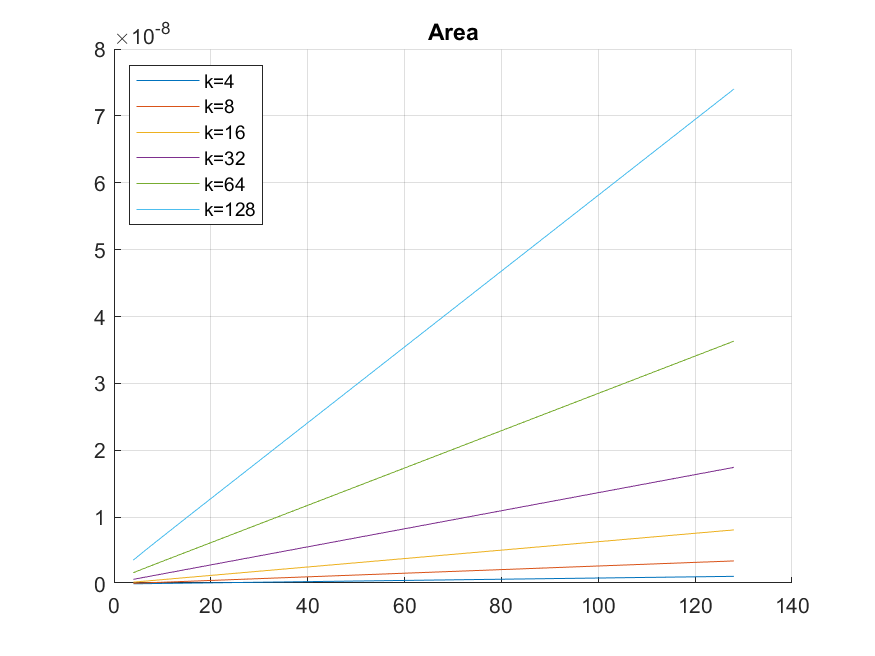
\includegraphics[width=9cm]{immagini/radix2ppipe0/area.png}
					\caption{Non-pipelined version}
				%				\label{fig:area}
			\end{subfigure}
			\begin{subfigure}{0.55\textwidth}
				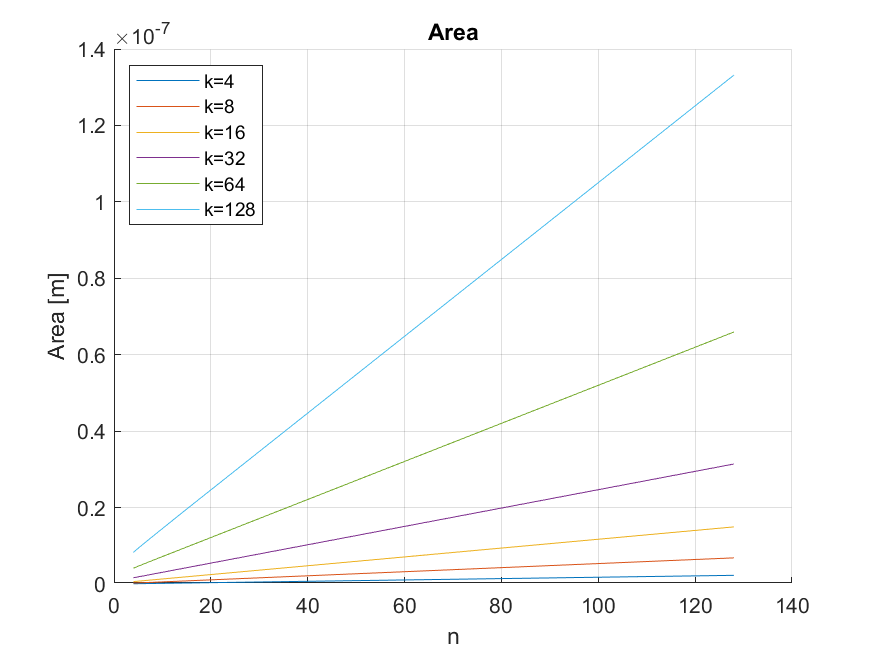
\includegraphics[width=9cm]{immagini/radix2ppipe2/area.png}
				\caption{50\%-Pipelined version}
%				\label{fig:3D area}
			\end{subfigure}
		
}{
		\begin{subfigure}{0.55\textwidth}
			\includegraphics[width=8cm]{immagini/radix2ppipe0/area3D.png}
			\caption{Non-pipelined version}
			%				\label{fig:area}
		\end{subfigure}
		\begin{subfigure}{0.55\textwidth}
			\includegraphics[width=8cm]{immagini/radix2ppipe2/area3D.png}
			\caption{50\%-Pipelined version}
			%				\label{fig:3D area}
		\end{subfigure}
	}
	\caption{Area}
	\label{fig:Area}
\end{figure}
As expected, the total area of the tree linearly increases with the number of bits (n) per input operand (Figures \ref{fig:Area}). The higher the number of operands (k) is, the larger is the total amount of the occupied area because of the higher number of stages required for the calculation.

In particular in order to appreciate the differences between the two versions of the tree, some meaningful points have been reported in the following table.


\begin{center}
\begin{tabular}{cc|c|c|}
	\cline{3-4}
	\multicolumn{1}{l}{}               & \multicolumn{1}{l|}{} & \multicolumn{2}{c|}{\textbf{Occupied area {[}m\textasciicircum{}2{]}}} \\ \hline
	\multicolumn{1}{|c|}{\textbf{n}}   & \textbf{k}            & \textbf{Non-pipelined}            & \textbf{50\% pipelined}            \\ \hline
	\multicolumn{1}{|c|}{\textbf{4}}   & \textbf{4}            & 3.4e-11                           & 6.504e-11                          \\ \hline
	\multicolumn{1}{|c|}{\textbf{4}}   & \textbf{128}          & 2.499e-9                          & 8.278e-9                           \\ \hline
	\multicolumn{1}{|c|}{\textbf{128}} & \textbf{4}            & 1.15e-9                           & 2.267e-9                           \\ \hline
	\multicolumn{1}{|c|}{\textbf{128}} & \textbf{128}          & 7.28e-8                           & 1.332e-7                           \\ \hline
\end{tabular}

\end{center}
As expected, the occupied area increases in the pipelind case since different levels of Flip flops are inserted; this increase becomes more and more significant as the number of bits and operands increase.



\subsection{Delay}

The delay is the time interval necessary to complete the computation through the whole tree.
In the non-pipelined case the path is entirely combinatorial while in the pipelined version the critical path is splitted into shorter homogeneous paths. In this last case the delay is therefore computed as the product between the clock period (the critical path delay) and the number of the pipeline stages inserted.

\begin{figure}[H]
	\makebox[\textwidth][c]{
		\begin{subfigure}{0.55\textwidth}
			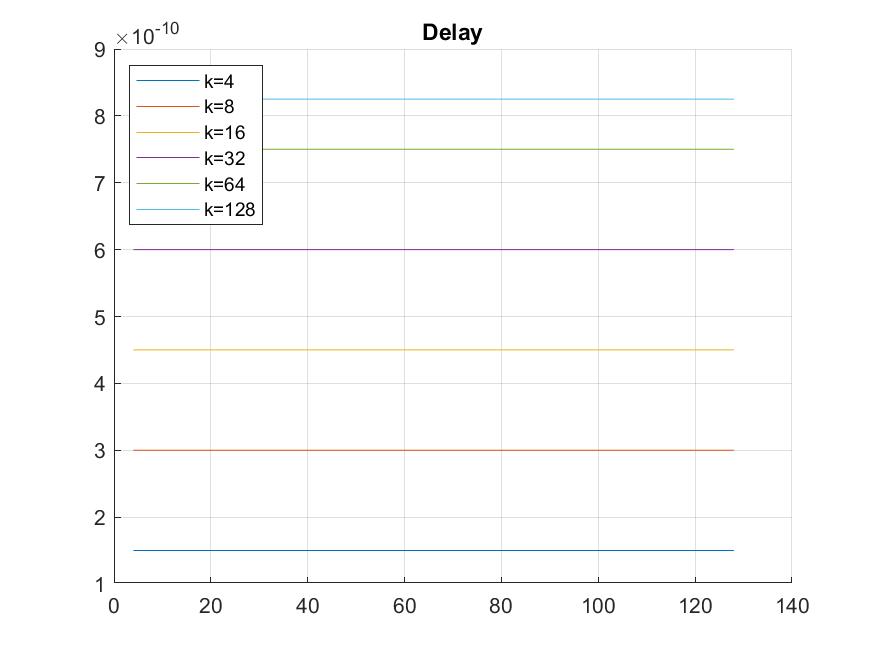
\includegraphics[width=9cm]{immagini/radix2ppipe0/delay.png}
			\caption{Non-pipelined version}
			%				\label{fig:area}
		\end{subfigure}
		\begin{subfigure}{0.55\textwidth}
			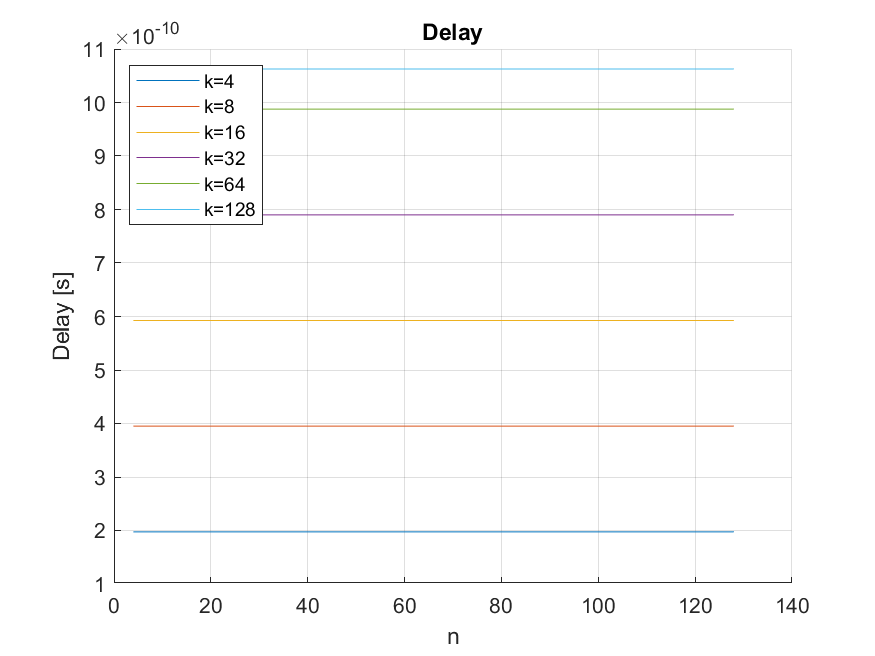
\includegraphics[width=9cm]{immagini/radix2ppipe2/delay.png}
			\caption{50\%-Pipelined version}
			%				\label{fig:3D area}
		\end{subfigure}
	}
{
		\begin{subfigure}{0.55\textwidth}
			\includegraphics[width=8cm]{immagini/radix2ppipe0/delay3D.png}
			\caption{Non-pipelined version}
			%				\label{fig:area}
		\end{subfigure}
		\begin{subfigure}{0.55\textwidth}
			\includegraphics[width=8cm]{immagini/radix2ppipe2/delay3D.png}
			\caption{50\%-Pipelined version}
			%				\label{fig:3D area}
		\end{subfigure}
	}
	\caption{Delay}
	\label{fig:Delay}
\end{figure}

As shown in Figure \ref{fig:Delay}, the amount of delay increases with the number of input operands, instead it is constant with respect to the number of bits. Since in each stage of the tree, full adders and half adders work in parallel, an higher input parallelism does not affect the total delay.

Once again, in order to appreciate the differences between the two versions of the tree, the delay has been computed for a growing number of operands.

\begin{center}
	\begin{tabular}{c|c|c|}
		\cline{2-3}
		\textbf{}                          & \multicolumn{2}{c|}{\textbf{Delay {[}ns{]}}}     \\ \hline
		\multicolumn{1}{|c|}{\textbf{k}}   & \textbf{Non-pipelined} & \textbf{50\% pipelined} \\ \hline
		\multicolumn{1}{|c|}{\textbf{4}}   & 0.15                   & 0.198                   \\ \hline
		\multicolumn{1}{|c|}{\textbf{8}}   & 0.3                    & 0.395                   \\ \hline
		\multicolumn{1}{|c|}{\textbf{16}}  & 0.45                   & 0.593                   \\ \hline
		\multicolumn{1}{|c|}{\textbf{32}}  & 0.6                    & 0.79                    \\ \hline
		\multicolumn{1}{|c|}{\textbf{64}}  & 0.75                   & 0.988                   \\ \hline
		\multicolumn{1}{|c|}{\textbf{128}} & 0.825                  & 1.063                    \\ \hline
	\end{tabular}
\end{center}

As expected, it is possible to notice how the delay increases in the pipelined case because of the overhead introduced by the registers stages. In particular, as k increases, also the number of levels of the tree increases and so more stages of flip flops are introduced.

\subsection{Static power}

Static power increases with both the number of bits and  the number of operands. This is trivial to understand why both of them depend on the total equivalent capacitance of the tree.
\begin{figure}[H]
	\makebox[\textwidth][c]{
		\begin{subfigure}{0.55\textwidth}
			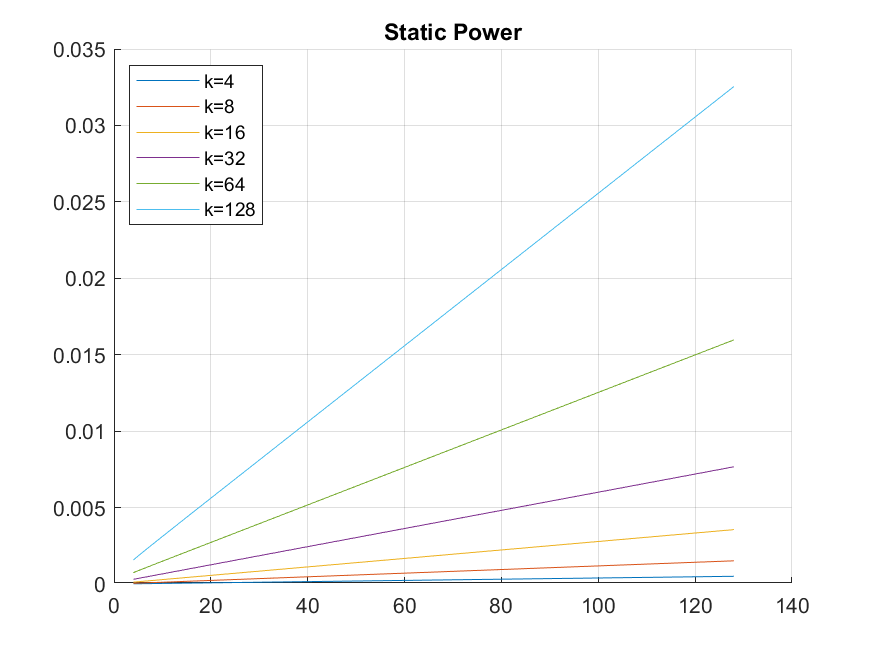
\includegraphics[width=9cm]{immagini/radix2ppipe0/p_static.png}
			\caption{Non-pipelined version}
			%				\label{fig:area}
		\end{subfigure}
		\begin{subfigure}{0.55\textwidth}
			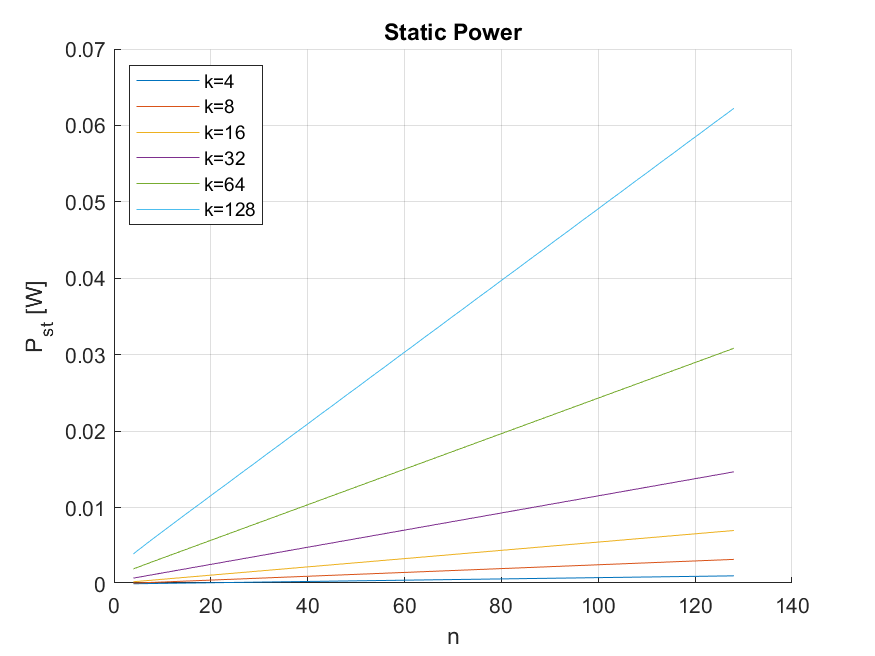
\includegraphics[width=9cm]{immagini/radix2ppipe2/p_static.png}
			\caption{50\%-Pipelined version}
			%				\label{fig:3D area}
		\end{subfigure}
	}
	{
		\begin{subfigure}{0.55\textwidth}
			\includegraphics[width=8cm]{immagini/radix2ppipe0/p_static3D.png}
			\caption{Non-pipelined version}
			%				\label{fig:area}
		\end{subfigure}
		\begin{subfigure}{0.55\textwidth}
			\includegraphics[width=8cm]{immagini/radix2ppipe2/p_static3D.png}
			\caption{50\%-Pipelined version}
			%				\label{fig:3D area}
		\end{subfigure}
	}
	\caption{Static power}
	\label{fig:pstat}
\end{figure}

Some quantitative evaluations are reported in the table below.

\begin{center}
	\begin{tabular}{cc|c|c|}
		\cline{3-4}
		\multicolumn{1}{l}{}               & \multicolumn{1}{l|}{} & \multicolumn{2}{c|}{\textbf{Static power {[}W{]}}} \\ \hline
		\multicolumn{1}{|c|}{\textbf{n}}   & \textbf{k}            & \textbf{Non-pipelined}  & \textbf{50\% pipelined} \\ \hline
		\multicolumn{1}{|c|}{\textbf{4}}   & \textbf{4}            & 1.495e-5                & 3.078e-5                \\ \hline
		\multicolumn{1}{|c|}{\textbf{4}}   & \textbf{128}          & 1.1e-3                  & 3.933e-3                \\ \hline
		\multicolumn{1}{|c|}{\textbf{128}} & \textbf{4}            & 5.057e-4                & 1.067e-3                \\ \hline
		\multicolumn{1}{|c|}{\textbf{128}} & \textbf{128}          & 3.2e-2                  & 6.224e-2                \\ \hline
	\end{tabular}
\end{center}

The pipelined version, again, is characterized by a larger static power consumption with respect to the non pipelined version since also the power consumption of the flip flops has been taken into account. 


\subsection{Dynamic power}
In order to make a proper comparison, dynamic power estimation has been performed for both versions of the tree considering an operating frequency of 5GHz.
\begin{figure}[H]
	\makebox[\textwidth][c]{
		\begin{subfigure}{0.55\textwidth}
			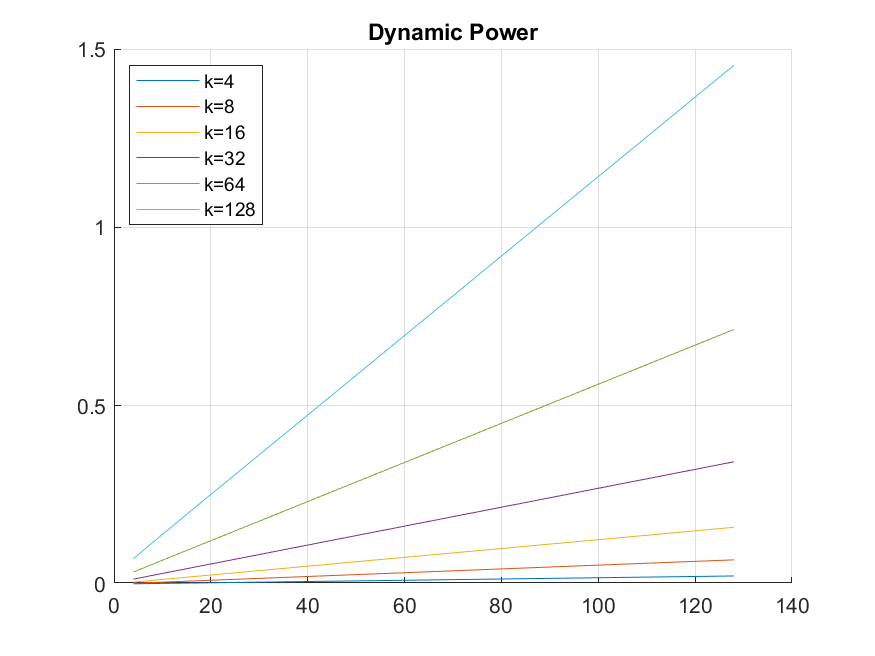
\includegraphics[width=9cm]{immagini/radix2ppipe0/p_dyn.png}
			\caption{Non-pipelined version}
			%				\label{fig:area}
		\end{subfigure}
		\begin{subfigure}{0.55\textwidth}
			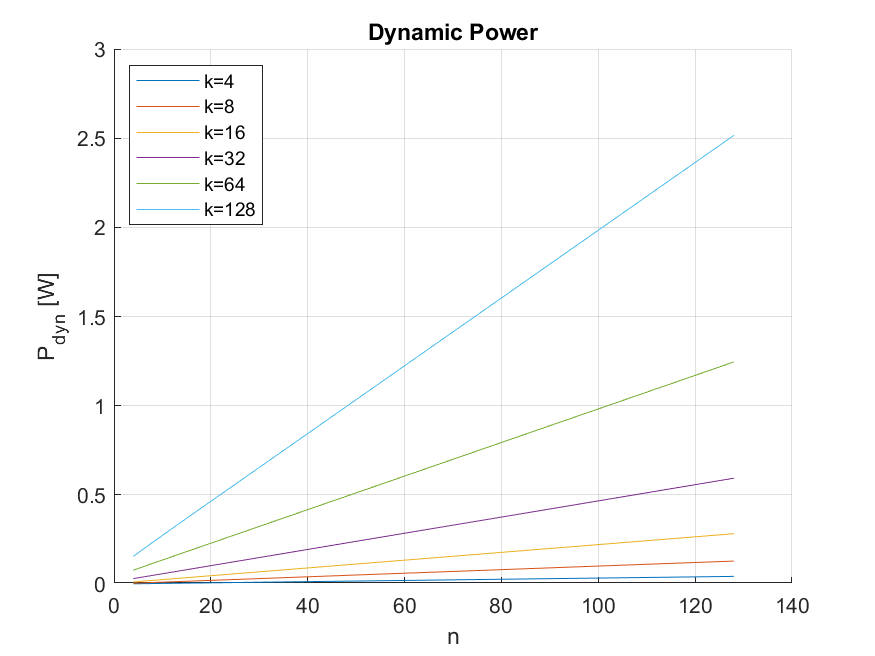
\includegraphics[width=9cm]{immagini/radix2ppipe2/p_dyn.png}
			\caption{50\%-Pipelined version}
			%				\label{fig:3D area}
		\end{subfigure}
	}
	{
		\begin{subfigure}{0.55\textwidth}
			\includegraphics[width=8cm]{immagini/radix2ppipe0/p_dyn3D.png}
			\caption{Non-pipelined version}
			%				\label{fig:area}
		\end{subfigure}
		\begin{subfigure}{0.55\textwidth}
			\includegraphics[width=8cm]{immagini/radix2ppipe2/p_dyn3D.png}
			\caption{50\%-Pipelined version}
			%				\label{fig:3D area}
		\end{subfigure}
	}
	\caption{Dynamic power ($f_{ck}=5 GHz$)}
	\label{fig:pdyn}
\end{figure}

In order to appreciate the differences between the two versions of the tree, some meaningful points have been reported in the following table.
\begin{center}
	\begin{tabular}{cc|c|c|}
		\cline{3-4}
		\multicolumn{1}{l}{}               & \multicolumn{1}{l|}{} & \multicolumn{2}{c|}{\textbf{Dynamic power {[}W{]}}} \\ \hline
		\multicolumn{1}{|c|}{\textbf{n}}   & \textbf{k}            & \textbf{Non-pipelined}   & \textbf{50\% pipelined}  \\ \hline
		\multicolumn{1}{|c|}{\textbf{4}}   & \textbf{4}            & 6.681e-4                 & 1.218e-3                 \\ \hline
		\multicolumn{1}{|c|}{\textbf{4}}   & \textbf{128}          & 0.049                    & 0.155                    \\ \hline
		\multicolumn{1}{|c|}{\textbf{128}} & \textbf{4}            & 0.023                    & 0.043                    \\ \hline
		\multicolumn{1}{|c|}{\textbf{128}} & \textbf{128}          & 1.431                    & 2.516                    \\ \hline
	\end{tabular}
\end{center}

Also in this case the power consumption grows with the number of bits-per-operand (n) and with the number of operands (k). 
In particular if n increases, the number of flip flops per level also increases; if k increases, the number of the stages of the tree and therefore the number of pipeline stages to be inserted increase. For this reason the pipelined version consumes more than the non-pipelined one.

Besides performing power estimations considering an operating frequency selected by the user, the developed script also is able to compute the maximum operating frequency depending on the critical path. It is possible to use then this value to obtain the dissipated power amount in the case of working at maximum performance.
In particular, considering the technological parameters involved, the system is able to work up to a $f_{ckMax}$ of about 5.06 GHz.

\subsection{Different pipeline percentages comparison}
The developed Matlab code also uses a parameter called $ppipe$: it is linked to the percentage of pipelining to be applied at the tree, in particular it indicates every how many levels of the tree a pipe stage is introduced. For example:
\begin{itemize}
	\item if $ppipe=0$ no pipeline stages are introduced (non-pipelined version);
	\item if $ppipe=1$ a pipeline stage is inserted at every level of the tree (fully pipelined version, 100\%);
	\item if $ppipe=2$ a pipeline stage is inserted every 2 levels of the tree (50\%).
\end{itemize}
In Figure \ref{fig:ppipe} occupied area, delay, static and dynamic power estimations are shown in the case of n=128, k=128 and a varying value of ppipe.
It is possible to observe that the plots are similar. When ppipe=0 no flip flops are inserted in the design, this corresponds to the minimum area and power.
When ppipe=1 the design is fully pipelined and therefore here lies the maximum for both area and power.
As the pipeline percentage decreases (ppipe increases) the plots approximately follow the trend of a decreasing exponential.

\begin{figure}[H]
	\makebox[\textwidth][c]{
		\begin{subfigure}{0.55\textwidth}
			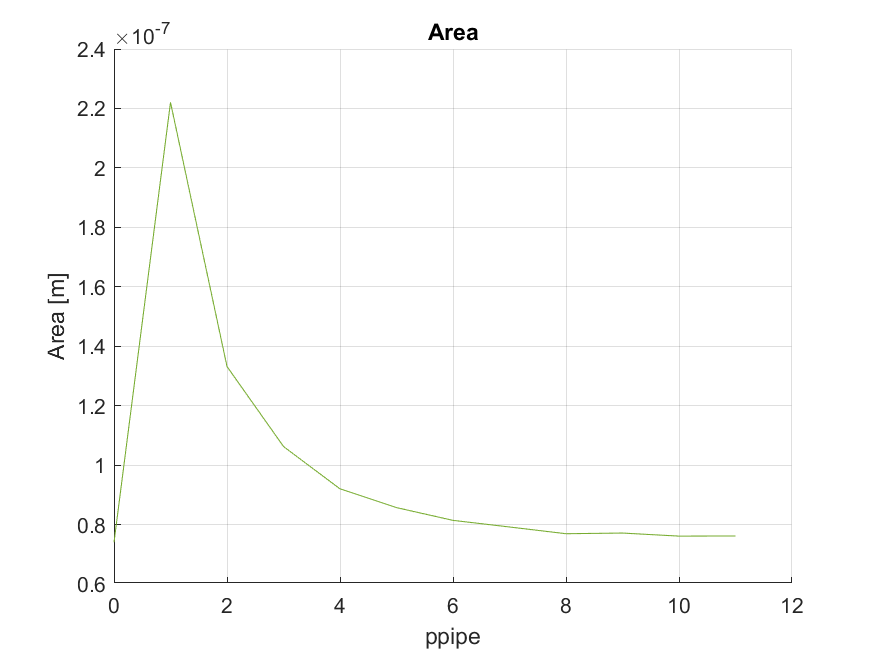
\includegraphics[width=9cm]{immagini/radix2ppipe2/area_pipe.png}
		\end{subfigure}
		\begin{subfigure}{0.55\textwidth}
			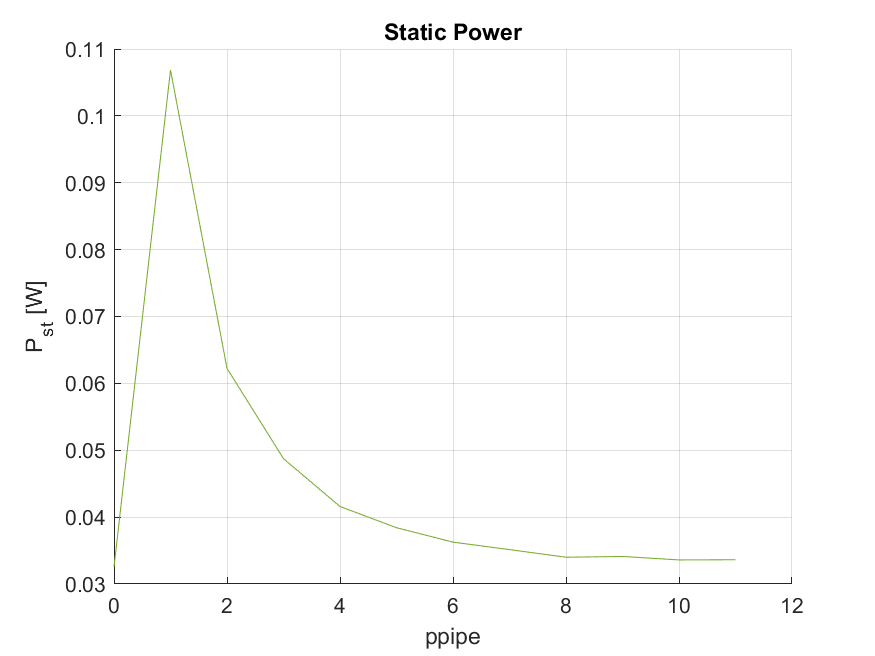
\includegraphics[width=9cm]{immagini/radix2ppipe2/p_static_pipe.png}
		\end{subfigure}
	}
{
		\begin{subfigure}{0.55\textwidth}
			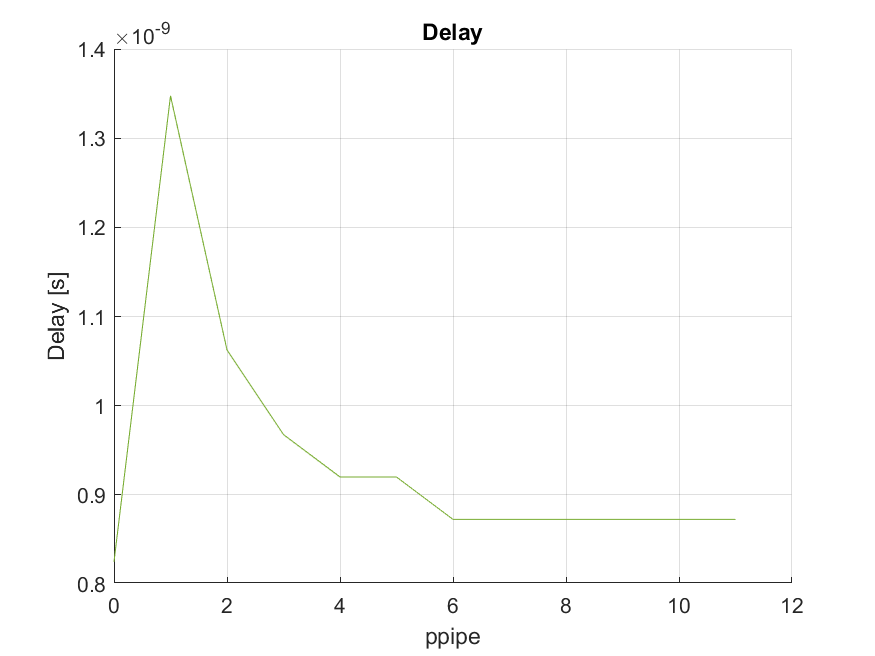
\includegraphics[width=9cm]{immagini/radix2ppipe2/delay_pipe.png}
		\end{subfigure}
		\begin{subfigure}{0.55\textwidth}
			\includegraphics[width=9cm]{immagini/radix2ppipe2/p_dyn_fmax_pipe.png}
		\end{subfigure}
	}
	\caption{Comparisons}
	\label{fig:ppipe}
\end{figure}
Considering the delay, in particular it is possible to notice how the behaviour does not strictly follow the one of the other 3 plots presented. The trend in this case is linked to the number of operands which determine the number of the levels of the tree. In this case since for 128 operands the number of levels is 11, starting from ppipe=6 the trend is perfectly flat: only one pipe level is inserted for ppipe$>$6 therefore the total delay of the tree is the same. Something similar happens for ppipe=4 and ppipe=5 but 2 register levels are added in this case.
It is therefore possible to notice how the optimal pipe percentage to be inserted in the tree depends on the number of operands.

\subsubsection{Throughput} In Figure \ref{fmax} is reported the throughput taking into account different pipeline depths cases. 

The trend is similar to the previous cases: the fully pipelined case (ppipe=1) is characterized by the highest possible throughput since the critical path is the one of a single FA. This allows to have multiple elaborations in execution at the same time (at different stages of the pipelined structure). With an increasing number of pipeline stages, latency (in terms of clock cycles needed to complete an elaboration) increases as well. 

\begin{figure}[H]
	\centering
	\includegraphics[width=10cm]{immagini/radix2ppipe2/fmax_pipe.png}
	\caption{Maximum throughput for different pipeline depths}
	\label{fmax}
\end{figure}
   
\subsection{VHDL}
The developed script also generates the VHDL description of the tree. The output design has been then verified through simulation. In Fig \ref{fig:schem} is shown the block diagram schematic for a simple tree with n=4, k=4 and ppipe=2.  

\begin{figure}[H]
	\includegraphics[trim={0 1.2cm 0 0},clip=true,scale=0.8]{./immagini/4x4.png}
	\caption{4x4 Wallace tree design (ppipe=2)}
	\label{fig:schem}
\end{figure}

The flip flop layer is placed after the second level of the tree, it has been included in the components $HA\_ff$ and $FA\_ff$.

\section{Conclusions}
It was developed a model of a Wallace tree with a percentage of pipelining which can be defined by the user. The present model also allows to not insert any pipeline stage. 
The main advantage of a pipelined implemantation lies in the fact that throughput increases while the time required to complete a single computation increases. 
Since flip flop insertion causes an increase of both area and power, it is therefore important to carefully choose how many pipeline stages should be inserted in the tree. 
The choice depends on the application, the optimal choice for the Wallace tree does not corresponds to a fully pipelined approach since it maximizes occupied area, consumptions and also latency.








\chapter{A Dynamic CMOS Survey}


Along with the work of the two adder designs, a brief survey about dynamic logic has been made. The main issue is to find whether there are new dynamic logic technologies that can be used in adders, instead of the standard static MOS structures. The main characteristics of dynamic logic are introduced and discussed, in order to understand the positive and negative aspects of this design technique. For further general information \cite{Rabaey} can be seen.

\section{General aspects}

\paragraph{} Dynamic logic is an alternative design approach of Pseudo NMOS and static CMOS and presents several advantages similar to these ones. Figure \ref{fig:dynamic} shows the general schematic of a dynamic logic topology. In this case a pull down network is used, just like the static CMOS logic, but the dual pull up network can be used instead.

\begin{figure}[H]
\centering
\includegraphics[width = 7 cm]{dinamic_logic_survey/Dynamic_logic-Page-1.png}
\caption{Dynamic logic general schematic.}
\label{fig:dynamic}
\end{figure}

\paragraph{} The first positive feature is the lower area occupation: the number of transistors increases linearly with the number of inputs. A generic dynamic N port gate has N+2 transistors, which is close to the pseudo NMOS design, and less than the static CMOS logic, which is 2N. The first N transistors are needed to implement the Pull Down (or Up) Network, while a PMOS and NMOS are used for the clock signal. The clock signal is needed to define the two working phases of the circuit, the pre-charge and the evaluation phases.

\paragraph{} Another important aspect is the absence of static power consumption, unlike pseudo NMOS but similar to the static CMOS logic. The static power is the generated power due to short path between supply voltage and ground.

\paragraph{} Furthermore, the circuit presents a lower fan-in with respect to the static CMOS implementation, and this aspect leads dynamic logic to better performance. These features together makes dynamic logic suitable for high performance and low cost implementation.

\paragraph{} The dynamic logic presents several drawbacks, though. The need of a clock signal affects negatively power consumption, since at least two transistors are charged and discharged in each clock cycle. Power consumption is also affected by an activity factor $\alpha_{1 \rightarrow 0}$ higher than the static CMOS. For example, if all the inputs of a NOR gate have a uniform statistic distribution, the activity factor of the dynamic logic and static logic implementations are, respectively the (\ref{alpha_dynamic}) and (\ref{alpha_static}):
\begin{equation}
\alpha_{dynamic} = 75\% \
\label{alpha_dynamic}
\end{equation}
\begin{equation}
\alpha_{static} = 18,75\%
\label{alpha_static}
\end{equation}
The dynamic power consumption is given by the (\ref{dynamic_power_consumption}):
\begin{equation}
P_{dyn} = \alpha\cdot C_L V_{dd}^2 f_{clk}
\label{dynamic_power_consumption}
\end{equation}
which is proportional to the activity factor. Leakage currents are to be considered also, since they can discharge the output node, and determine the minimum period between two pre-charge phases, which is the minimum clock frequency accepted. This value is about some KHz. Leakage currents tend to discharge the output node, since this one is an high impedance node. This problem can be resolved by using a \textit{bleeder} transistor \cite{Rabaey}.

\paragraph{} Another aspect to be considered is the charge sharing with other output and with the clock signal (\textit{clock feedthrough}) which affects dramatically reliability. The latter can forward bias the drain-bulk junction of the pre-charge MOS  which  can switch the high impedance node voltage from '1' to '0' or, worse, cause \textit{latch-up}.

\newpage
\section{Domino design techniques}
An evolution of dynamic logic is the Domino one, which was first described by \cite{Krambeck}. Figure \ref{fig:DOMINO} shows the schematic of a single stage Domino circuit.

\begin{figure}[H]
\centering
\includegraphics[width = 7 cm]{dinamic_logic_survey/Dynamic_logic-Page-2.png}
\caption{General schematic of domino logic circuit. The bleeder transistor is optional but highly recommended, in order to avoid information loss due to leakage currents.}
\label{fig:DOMINO}
\end{figure}

The main advantage is that Domino circuits can be placed in multiple stages with the same topology and can be pipelined with multiphase clocking system \cite{Verma} instead of using latches. At architectural level, the adoption of multiphase clocking prevent the use  High performance are reached at the expense of higher power consumption due to the more clock lines needed.


\section{Dual Rail Domino Logic}
A particularly and interisting case of Domino logic is the Dual Rail Domino Logic (DRDL) implementation in order to make low power adders \cite{dominoAdder8}. An example of Dual rail Domino circuit is reported in figure \ref{fig:Dual Rail}.
\begin{figure}[H]
\centering
\includegraphics[width = 7 cm]{dinamic_logic_survey/Dynamic_logic-Page-3.png}
\caption{Dual Rail Domino logic implementation of a NAND circuit. The main advantage is to have inverting and non inverting function, at the expense of more area occupation.}
\label{fig:Dual Rail} 
\end{figure}
In this implementation, circuit works in near threshold in order to reduce power consumption and uses an asynchronous pipeline. This approach reduces the energy-delay product, defined as:
\begin{equation}
EDP = E_{op} \times \tau_{delay}
\end{equation}
where $E_{op}$ is the energy drained by the device during the SPICE simulation and $\tau_{delay}$. Although there is an improvement in energy consumption, performance and area become worse than a synchronous pipelined static CMOS implementation. Energy consumption, number of transistors and delay of \cite{dominoAdder8} are reported in table \ref{tab:8bitAdder}. The worst case is used for synchronous adder and average case for the dual rail Domino logic one.
\begin{table}[H]
\centering
\begin{tabular}{|c|c|c|c|}
\hline 
 & Transistors & Delay $\mu s$ & Energy $fJ$ \\ 
\hline 
DRDL & 1460 & 62.6 & 499 \\ 
\hline 
CMOS & 764 & 59.3 & 871 \\ 
\hline 
\end{tabular}
\caption{Comparison between DRDL and static CMOS 8-bit adder.}
\label{tab:8bitAdder}
\end{table}
As it can be seen, energy consumption is improved with respect to CMOS at the cost of almost double area and a little worse delay.


\section{Technology scaling comparison}
An important issue is to find whether technology scaling improve significantly the Domino circuits power consumption with respect to static CMOS logic. Two interesting works are found are compared in table .
\begin{table}[H]
\centering
\begin{tabular}{|c|c|c|c|}
\hline 
 & Power & Pwr diff. with the previous gate \\ 
\hline 
32 nm FinFET static NAND2 in \cite{Nalamwar} & 440 nW & 0 \% \\ 
\hline 
25 nm FinFET Domino AND2 in \cite{Rasouli} & 1.6 $\mu W$ & +264 \% \\
\hline 
32 nm FinFET static NOR2 \cite{Nalamwar} & 440 nW & 0 \% \\ 
\hline 
25 nm FinFET Domino OR2 \cite{Rasouli} & 4 $\mu W$ & +810 \% \\ 
\hline 
\end{tabular} 
\end{table}
Despite of the use of a better technology, the Domino logic suffers for higher power consumption, compared with the static CMOS logic.

\section{Final Considerations}
Dynamic logic based circuits are a good alternative if area and performance are critical aspects of the design. Multistage Domino circuits can be also pipelined with a multiphase clock approach, so no more latches are needed and there is more area saving. These aspects are  balanced by a higher power consumption, which can be far higher than the static logic. Scaling does not improve the power consumption issue, so dynamic logic is generally not suitable for low power implementations, which is the current tendency. The Dual Rail Domino logic can be an interesting choice in case of asynchronous pipeline designs, since energy consumption is better than synchronous static implementations, although they occupy more area and have a performance similar to the static logic.
\bibliography{dinamic_logic_survey/references}	
\bibliographystyle{ieeetr}
\end{document}
